% This is a template for Ph.D. dissertations in the UCI format.
% 
% All fonts, including those for sub- and superscripts, must be 10
% points or larger.  Recommended sizes are 14-point for chapter
% headings, 12-point for the main body of text and figure/table
% titles, and 10-point for footnotes, sub- and super-scripts, and text
% in figures and tables.
%
% Notes: Add short title to figures, sections, via square brackets,
% e.g. \section[short]{long}.
%
\documentclass[12pt,fleqn]{ucithesis}

% A few common packages
\usepackage{amsmath}
\usepackage{amsthm}
\usepackage{array}
\usepackage{graphicx}
\usepackage{natbib}
\usepackage{relsize}

\usepackage{bibentry}    % Put full references in text
\usepackage{etoolbox}    % This line and the next are absolutely necessary to get \bibentry{} command to work in figure caption.
\robustify{\bibentry}

% Some other useful packages
\usepackage{caption}
\usepackage{subcaption}  % \begin{subfigure}...\end{subfigure} within figure
\usepackage{multirow}
\usepackage{tabularx}
\usepackage{siunitx}
\usepackage{amssymb}


% plainpages=false fixes the "duplicate ignored" error with page counters
% Set pdfborder to 0 0 0 to disable colored borders around PDF hyperlinks
\usepackage[plainpages=false,pdfborder={0 0 0}]{hyperref}



% Uncomment the following two lines to use the algorithm package,
% which provides an algorithm environment similar to figure and table
% ("\begin{algorithm}...\end{algorithm}"). A list of algorithms will
% automatically be added in the preliminary pages. Note that you
% probably want a package for the actual code to go with this (e.g.,
% algorithmic).
%\usepackage{algorithm}
%\renewcommand{\listalgorithmname}{\protect\centering\protect\Large LIST OF ALGORITHMS}

% Uncomment the following line to enable Unicode support. This will allow you
% to enter non-ASCII characters (such as accented characters) directly without
% having to use LaTeX's awkward escape syntax (e.g., \'{e})
% NOTE: You may have to install the ucs.sty package for this to work. See:
% http://www.unruh.de/DniQ/latex/unicode/
%\usepackage[utf8x]{inputenc}

% Uncomment the following to avoid "widowing", where page breaks cause
% single lines of paragraphs to float onto the next page (this is not
% a UCI requirement but more of an aesthetic choice).
%\widowpenalty=10000
%\clubpenalty=10000

% Modify or extend these at will.
\newtheorem{theorem}{\textsc{Theorem}}[chapter]
\newtheorem{definition}{\textsc{Definition}}[chapter]
\newtheorem{example}{\textsc{Example}}[chapter]

% Matrix
\newcommand{\matr}[1]{\mathbf{#1}}


% Macros for title, author, abstract, etc.
\thesistitle{Applications of Synthetic Microchannel and Nanopore systems}

\degreename{Doctor of Philosophy}

% Use the wording given in the official list of degrees awarded by UCI:
% http://www.rgs.uci.edu/grad/academic/degrees_offered.htm
\degreefield{Physics}

% Your name as it appears on official UCI records.
\authorname{Preston Hinkle}

% Use the full name of each committee member.
\committeechair{Dr. Zuzanna S. Siwy}
\othercommitteemembers
{
  Dr. Jun Allard \\
  Dr. Ilya Krivorotov
}

\degreeyear{2017}

\copyrightdeclaration
{
  {\copyright} {\Degreeyear} \Authorname
}

% If you have previously published parts of your manuscript, you must list the
% copyright holders; see Section 3.2 of the UCI Thesis and Dissertation Manual.
% Otherwise, this section may be omitted.
% \prepublishedcopyrightdeclaration
% {
% 	Chapter 4 {\copyright} 2003 Springer-Verlag \\
% 	Portion of Chapter 5 {\copyright} 1999 John Wiley \& Sons, Inc. \\
% 	All other materials {\copyright} {\Degreeyear} \Authorname
% }

% The dedication page is optional.
\dedications
{
	
}

\acknowledgments
{
	
}


% Some custom commands for your list of publications and software.
\newcommand{\mypubentry}[3]{
  \begin{tabular*}{1\textwidth}{@{\extracolsep{\fill}}p{4.5in}r}
    \textbf{#1} & \textbf{#2} \\ 
    \multicolumn{2}{@{\extracolsep{\fill}}p{.95\textwidth}}{#3}\vspace{6pt} \\
  \end{tabular*}
}
\newcommand{\mysoftentry}[3]{
  \begin{tabular*}{1\textwidth}{@{\extracolsep{\fill}}lr}
    \textbf{#1} & \url{#2} \\
    \multicolumn{2}{@{\extracolsep{\fill}}p{.95\textwidth}}
    {\emph{#3}}\vspace{-6pt} \\
  \end{tabular*}
}

% Include, at minimum, a listing of your degrees and educational
% achievements with dates and the school where the degrees were
% earned. This should include the degree currently being
% attained. Other than that it's mostly up to you what to include here
% and how to format it, below is just an example.
\curriculumvitae
{

\textbf{EDUCATION}
  
  \begin{tabular*}{1\textwidth}{@{\extracolsep{\fill}}lr}
    \textbf{Doctor of Philosophy in Physics} & \textbf{2017} \\
    \vspace{6pt}
    University of California, Irvine & \emph{Irvine, California} \\
    \textbf{Bachelor of Science in Physics} & \textbf{2011} \\
    \vspace{6pt}
    The Ohio State University & \emph{Columbus, Ohio} \\
  \end{tabular*}

\vspace{12pt}
\textbf{RESEARCH EXPERIENCE}

  \begin{tabular*}{1\textwidth}{@{\extracolsep{\fill}}lr}
    \textbf{Graduate Student Researcher} & \textbf{2012--2017} \\
    \vspace{6pt}
    University of California, Irvine & \emph{Irvine, California} \\
  \end{tabular*}

\vspace{12pt}
\textbf{TEACHING EXPERIENCE}

  \begin{tabular*}{1\textwidth}{@{\extracolsep{\fill}}lr}
    \textbf{Teaching Assistant} & \textbf{2012--2016} \\
    \vspace{6pt}
    University of California, Irvine & \emph{Irvine, California} \\
  \end{tabular*}
  
   \begin{tabular*}{1\textwidth}{@{\extracolsep{\fill}}lr}
    \textbf{Teaching Assistant} & \textbf{2012} \\
    \vspace{6pt}
    The Ohio State University & \emph{Columbus, Ohio} \\
  \end{tabular*}


  
\pagebreak

\textbf{REFEREED JOURNAL PUBLICATIONS}

	\bibentry{Hinkle2017}
	\bibentry{Yang2016}
	\bibentry{Qiu2015}

% \vspace{12pt}
% \textbf{REFEREED CONFERENCE PUBLICATIONS}
% 
% 	\mypubentry{Awesome paper}{Jun 2011}{Conference name}
% 	\mypubentry{Another awesome paper}{Aug 2012}{Conference name}

\vspace{12pt}
\textbf{SOFTWARE}

  \mysoftentry{nanoIV}{https://github.com/tphinkle/nanoIV}
  {Keithley 6487 Picoammeter control GUI program. Allows measurement of current-voltage and time-series data.}
  
  \mysoftentry{pore stats}{https://github.com/tphinkle/pore_stats}
  {GUI program and Python library for extracting and analyzing resistive pulse data.}
  
  
}

% The abstract should not be over 350 words, although that's
% supposedly somewhat of a soft constraint.
\thesisabstract
{
	There are a diverse range of applications involving fluidic systems at the micro- and nanoscale. Making use of the nanoscale physics that takes place in the vicinity of charged surfaces, there is the possibility that nanopores, holes on the order of $\SI{1}{nm}$ in size, could be used to make complex integrated ionic circuits. For inspiration on what such circuits could achieve we only need to look to biology systems, immensely complex machines that at their most basic level require precise control of ions and intercellular electric potentials to function. In order to contribute to the ever expanding field of nanopore technology, we engineered novel hybrid insulator-conductor nanopores that behave analagously to ionic diodes, which allow passage of current flow in one direction but severely limit the current in the opposite direction. Not only did the behavior of the pore give key insights into the fundamental physics and chemistry underlying the electrical double layer, but it can also be considered as a standard rectifying element in ionic circuits. Another application of ion conducting channels is a particle sensing method, known as resistive pulse sensing. We present three main experiments that expand the capacity of resistive pulse sensing applications. First, we demonstrate how resistive pulse sensing in pores with longitudinal irregularities can be used to measure the lengths of individual nanoparticles. Then, we describe an entirely new hyridized method, whereby resistive pulse sensing is combined with optical imaging. The hybrid method allows for validation of the resistive pulse signals, and will greatly contribute to their interpretability. We present experiments that explore some of the possibilities of the hybrid method. Then, building off the hybrid method we present our findings for experiments performed with using resistive pulse sensing to measure the deformability of particles. Using a novel microfluidic channel design, we were able to reproducibily induce deformation of cells in a controlled manner. We describe how these deformations could be detected with the resistive pulse signal, paving the way for resistive pulse sensing based cell deformability cytometers.
}


%%% Local Variables: ***
%%% mode: latex ***
%%% TeX-master: "thesis.tex" ***
%%% End: ***


% Add PDF document info fields
\hypersetup{
	pdftitle={\Thesistitle},
	pdfauthor={\Authorname},
	pdfsubject={\Degreefield},
}


%\theoremstyle{definition}
%\newtheorem{definition}{Definition}[section]
 
%\theoremstyle{remark}
%\newtheorem*{remark}{Remark}

% Uncomment the following to have numbered subsubsections (by default
% numbering goes only to subsections).
%\setcounter{secnumdepth}{4}


% Set this to only select a subset of the includes directives below.
% Very handy to speed up compilation if you're working on a certain
% part of your thesis. It conserves page numbers, references, etc.
% even for non-included files.
%\includeonly{chapter1}

\begin{document}

% Preliminary pages are always loaded (TOC, CV, etc.)
\preliminarypages

% Include the different components of your thesis, in separate files.
% Using \include allows you to set \includeonly above.

\nobibliography*

\graphicspath{{../images/ch1/}}	% Image directory


\chapter{Introduction}

	The introduction to this dissertation is structured as follows. First, we introduce the main topic of this dissertation and of my PhD research work, the nanopore. This section serves to introduce the reader first, to the basic definition of a nanopore and then to some of their applications, in addition to miscellaneous facts about nanopores that provide context for why they are of interest to scientists. This section is entirely qualitative and does not aim to make any statements about the underlying physics needed to understand nanopore systems. Subsequently, I introduce in three stages the physics that is relevant to nanopore systems. It turns out that if we take a macroscaled system (say, a tube rather than a nanotube) and slowly shrink it in size, then as the system size shrinks new types of physics emerges and become increasingly relevant to the system. We will start by addressing the relevant physics at the milliscale and shrink in intervals of powers of three, stopping at the sub-nanoscale. Therefore, the progression looks like milli-, micro-, nano-, and finally, sub-nano-. To provide a bigger picture of the journey through different length scales, the progression looks like ant, cell, protein, molecule.

	\section{Nanopores}

		Unlike most physics jargon, the name nanopore is entirely self-explanatory. In fact, the following is a terse (but accurate) definition of a nanopore:


		\begin{definition} \label{def:nanopore}
			A nanopore is a hole on the order of $\SI{1}{nm}$ in size
		\end{definition}


		As we will discover, this definition, while accurate, does not do justice to the field of nanopore research. 

		Nanopores generally belong to two classes, biological and synthetic. Because nanopores can be found in biology, many scientists are interested in studying them in their own right, to better understand how biological systems function. On the other hand, nanopores, both biological and synthetic, can be used in a surprisingly large variety of applications, with the total count of such applications constantly increasing. In this section we will briefly discuss the types of biological nanopores and where they are found in nature, and then move on to describing different types of synthetic nanopores. Given the loose criteria required by \ref{def:nanopore} for something to constitute a nanopore, listing off every type of either biological or synthetic nanopores would be impossible; instead, I seek to introduce the most relevant types, with an admitted bias towards the types of nanopores I am most familiar with and that I have worked with in my research. After discussing the various types of nanopores, I will give a summary of applications in which nanopores see use. Some of these applications, for instance resistive-pulse sensing, are a major part of this dissertation and will therefore be discussed in much greater detail later on, while others, such as DNA sequencing, are important enough to be mentioned but not discussed in significant detail later on. An extensive list of references, including those not explicitly referenced in this work, will be included should the reader wish to read more on a particular topic.

		\begin{figure}[h]
			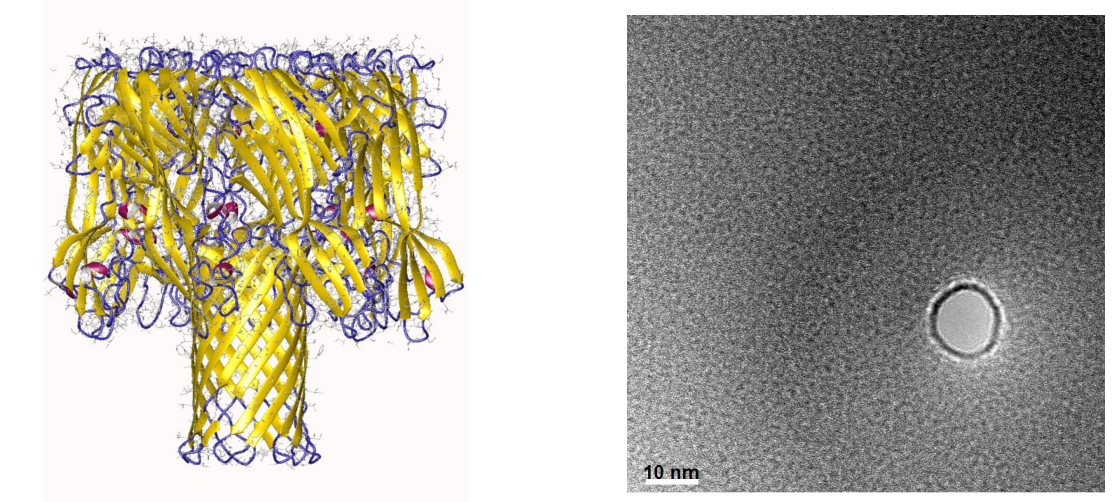
\includegraphics[width=\textwidth]{bio_synth_nanopores.png}
			\caption{Two types of nanopores. \textbf{Left:} Alpha-hemolysin, a biological type of nanopore approximately $\SI{1}{nm}$ in diameter. \textbf{Right:} A silicon nitride nanopore drilled using a transmission electron microscope (TEM), approximately $\SI{10}{nm}$ in diameter.}
		\end{figure}

		\subsection{Biological nanopores}

			As mentioned before, nanopores exist naturally in biology. Their most important function is to enable passage from one region to another, much like a tunnel does; however, where a tunnel permits cars, trucks, etc., the passengers in nanopore systems are water, ions, proteins, etc. Nanopores typically connect regions that are necessarily divided in order for a cell to function. Membrane-bound nanopores are structures made out of protein that are embedded in a cell's lipid bilayer that connect the outside of a cell to the inside of a cell. They serve the useful function of regulation osmotic pressure by allowing water to enter and exit the cell, and also balance voltage differences by allowing passage of important electrolytes such as sodium, potassium, and chloride. Therefore, maintaining homeostasis is one of the chief functions of these types of nanopores. These pores also enable passage of messenger molecules that enable extracellular messenging, crucial to all multicelled organisms. Like lipid bilayer pores, there are also pores in the nuclear membrane that enable transport into and out of the nucleus of a cell. These pores' chief responsibility is to allow the passage of messenger molecules in and out of the nucleus. 

			The most fascinating property of nanopores is their capacity for active management of transport. For instance, some nanopores may open or close when the voltage difference across them surpasses a threshold; other types of nanopores are \textit{ion selective}, permitting passage of some types of ions while denying passage to others. \textit{Active} transport is absolutely crucial to biological systems; if all nanopores were passive holes that permitted anything to pass through, the system would equilibrate in a homogeneous, non-functional soup of maximum entropy---life simply could not exist. Fortunately for us, nanopores are active transport regulators and life goes on. Going back to our tunnel analogy, nanopores act more like regulated tunnels, for instance some with guards that permit small cars only and deny trucks, or permit passage in only one direction, etc.

		\subsection{Synthetic nanopores}

			Advances in nano- and microfabrication have led to an enormous number of different types of synthetic nanopores. Synthetic nanopores can be made from a variety of different types of materials, and often their geometry (shape and size), as well as their surface chemistry properties, can be tailored to introduce specific types of behavior. However, the type of material used to make the nanopore most often determines the types of geometries and chemistries that are allowed. The following is a list of common types of nanopores, with a description of the type of material they are made from, their permissable length scales, and other miscellaneous relevant facts about them.

			\textbf{Monolayer pores.} The invention of graphene, a monolayer of carbon atoms, and later MoS2, opened the possibility of creating nanopores with a length of a single atom. These types of pores are created by punching through the thin monolayer, typically with an electron or ion beam. While still a very new field of study, these pores may see future use in desalination (removing electrolyte ions from water).

			\textbf{Carbon nanotubes.} A carbon nanotube can be conceptually understood as a rolled up tube of one or a stack of graphene layers. Graphene is a a monolayer of carbon atoms, and therefore a carbon nanotube itself is a type of pure crystal structure. The lattice arrangement of carbon atoms permits only certain tube diameters, which itself depends on the chirality of the tube (the way the tube is rolled up). Carbon nanotubes are interesting to researchers because of the exotic behaviors they exhibit that are not present in most other types of nanopores---for instance, they exhibit frictionless transport of water, hydrogen-dominant conductance (\textit{via} the Grotthus mechanism), ion selectivity, and more. As of the submission of this dissertation, the use of CNTs as nanopore is still a new field of study, and the physical mechanism for the previously mentioned behaviors is still poorly understood. Nevertheless, the extreme confinement ($\SI{1}{nm}$ and below for small CNTs) and the atomic-level precision of their structure are believed to be responsible. Another interesting aspect of the smallest CNTs is the breakdown of mean-field physics in describing their behavior. For instance, the Navier-Stokes equations which describe fluid dynamics, breaks down at this level because the water must be considered at the molecular level; the mean-field approach is no longer valid. Because they are still new, we do not yet know the exact applications that these nanopores will see use in. However, it is likely that they could be used in desalination applications (removing ions from water), or in ionic circuits as cation selective elements.

			\textbf{Silicon nitride.} Silicon nitride is a type of crystalline semiconductor that permits engineering of nanopores through several different fabrication processes. Briefly, very thin layers of silicon nitride (e.g.~$10-100$ nm) are grown, and a hole is bored through via either electron or ion beam milling. For instance, in one project of this dissertation I describe a project conducted with silicon nitride pores that were drilled via high-energy transmission electron microscope (TEM). Depending on the type of mill used (ion or electron), the size of these nanopores ranges, but the diameter is generally in the range of $1-100$ nm. One advantage of silicon nitride pores is their smooth interior geometries, as well as the native silane chemistry on the surface that permits many types of chemical modifications. These types of pores are used as ionic rectifiers (after modification), and in resistive pulse applications.

			\textbf{Glass nanopipettes.} Quartz pipettes can be heated and slowly stretched, reducing the tip diameter with the possibility of reaching the nanoscale. Unlike the previously mentioned pores which all had an approximately cylindrical geometry, these nanopipettes have a conical shape. These pores have a couple advantages. First, the stretching process itself is simple and can be used to create many pores over a short amount of time. Second, the surface chemistry of the glass or quartz is amenable towards chemical modification. These pores may be used in ionic circuits, in resistive pulse sensing, or as a surface probe, by monitoring the current through the pipette as it approaches a charged surface.

			\textbf{Track-etched polymer nanopores.} These types of pores are perhaps the most robust, dependable types of nanopores. Pore formation is a multistep process. First, untouched polymer membranes are irradiated by a single heavy isotope of an element such as gold and xenon, that has been accelerated to high speeds in a particle accelerator. The ion rips through the membrane, uniformly dispersing some of its kinetic energy into the surrounding polymer, and breaking the bonds in the polymer surrounding its trajectory. This location of damaged polymer bonds is known as the `damage track'. An ion detector is placed at the exit point of the membranes so that the beam can be switched off when a single ion is detected. This detection, along with a solid mask placed in front of the beam that blocks the vast majority of the ions in the beam, ensures that films that only have a single damage track can be prepared. This step, known as irradiation, must be performed off-site at a particle accelerator. After heavy ion irradiation, the membranes are immersed in an etchant solution such as NaOH or KOH. The etchant preferentially attacks the polymer in the damage track, clearing out the polymers along the track much faster than elsewhere in the membrane. Once the track has been etched out, the rest of the membrane is isotropically etched slowly by the NaOH. Pores prepared by the track-etch technique have a few advantages, including a customizable size and geometry. By putting etching solution on only one side of the membrane, it is possible to create conical pores of various aspect ratios. By applying a voltage across the pore during the etching process, the ionic current can be monitored and the etching process can be stopped at a particular current level, allowing the researcher customize the pore diameter. Another advantage of these pores is the carboxyl groups native to their surfaces, which permit many types of useful chemical modifications.

			\textbf{Hybrid biological-synthetic nanopores.} Biological nanopores, such as alpha hemolysin, aerolysin, or MSPA to name a few, can be isolated from their host biological systems and inserted into synthetic systems, forming a hybrid biological-synthetic complex. In these cases, the pore is entirely biological, but the complex does not appear naturally in nature, and the pores may be used in engineering or scientific applications. To make matters even more confusing, such pores may also be genetically modified to change some of their behavior, meaning they are derived from biology but are synthesized in the lab. For instance, the company Oxford nanopore invented a genetically modified alpha hemolysin nanopore that is especially adept at differentiating between nucleotides, and is currently being used in DNA sequencing applications.

		\subsection{Applications (introductions)}

			So far, I have hinted at or referred to nanopore applications without getting into specifics. Just as there are too many types of nanopores to enumerate, there are too many applications of nanopores to list them all off. This is a list of some of the most important applications of nanopores.

			\textbf{Analyte detection and characterization with the resistive pulse technique.} Surprisingly, nanopores may be used as a sort of particle characterizer using something called the resistive pulse technique, which works as follows. A voltage is applied across the nanopore, which induces a measurable ionic current to flow through the channel. If a particle enters the nanopore, the particle will occupy a volume that otherwise would be occupied by high-conductivity ions, increasing the pore's resistance, and decreasing the measured current. It turns out that by studying the nature of the decrease in the current, we can gather some information about the transiting particle. For instance, by counting the number of pulses in the measured ionic current, we can determine the concentration of particles in the suspension. The size of the particle can be determined by relating it to the depth of the pulse---larger particles block the current to a larger degree, and therefore create deeper resistive pulses. If the particle is at least partially driven through the channel \textit{via} electrophoresis (discussed later), then the particle's surface charge can be determined by the length of the pulse, or `dwell time' of the particle.

			One advantage of resistive pulse sensing is its scale-independence, which is a result of the generality of the physics involved. For this reason, resistive pulse sensing has been used in a large number of applications. The original use of the resistive pulse technique was in performing red blood cell counts (channel size approximately $\sim\SI{100}{\mu m}$ which was achieved by Coulter in 1953; this is the reason why sometimes the resistive pulse technique is referred to as the Coulter counter priniciple, or simply the Coulter principle. Since Coulter's original design, the resistive pulse technique has been used in counting smaller specimens such as exosomes, proteins, and viruses, used to measure particle rigidity, and perhaps most importantly, in DNA sequencing. The basic idea of resistive-pulse sensing for DNA sequencing is that the four types of nucleotides have slightly different sizes, and therefore lead to four unique current blockages. DNA can be slowly threaded through a nanopore while the current is monitored, and the discrete states in the resulting time-series of the measured current yield the sequence of DNA.

			\textbf{Water desalination.} Charged nanopores are slightly ion selective, meaning they preferentially allow one polarity of charge over another to pass through. If one side of a nanopore membrane is filled with electrolyte solution and a pressure is applied, water will pass through the pore, and due to the selectivity of the membrane, fewer ions will pass through than are contained in the bulk. In this way, nanopores can be used for water desalination. This mechanism of salt rejection is electrostatic, since the finite potential in the vicinity of the pore walls is responsible for screening ions. Traditional water desalination relies on reverse osmosis membranes that are completely impermeable to salts, and therefore \textit{sterically} reject ions.  In future sections we will discuss the physics involved with water desalination.

			\textbf{Nanopore ionics and ionic circuits.} Ion transport is fundamentally important to all cellular life. At the most basic level, single cells maintain homeostasis with their environment by maintaining a careful balance of salt ions across their membranes. This balance is regulated by a rich variety of ion channels, each with their own specific functionality. For instance, potassium can diffuse through potassium channels at nearly the bulk diffusion rate (i.e. the channel hardly impedes their motion), while sodium is completely blocked, an amazing feat considering the ions are nearly identical, save a minute difference in their hydration radii. Beyond maintaining homeostasis, ion channels are also responsible for propagating electric signals along axons, crucial for signaling in multicellular organisms. 

			One of the holy grails in nanopores is being able to reproduce the functionality of these biological pores, that were created by millions or billions of years of evolution, in synthetic systems. The ability to do so could create a revolution in ion conducting systems, analagous to the revolution in electronics that was created by the invention of the solid-state transistor. However, the goal of ionics is not to replace wires, capacitors, and transistors with ion channels and pores; indeed, ions travel orders of magnitude slower than electrons, and therefore ionic systems are expected to act more slowly than electronic systems. Instead, integrated ionic circuits could be used for complex signaling since each ion carries its own information, and for controlling the transport of biomolecules. One needs only to look at biology for inspiration on the application of complex ion channels.

	\section{Nanopore science---physics and chemistry}

		The actors at play in nanopore systems include the fluid solvent that fills the pore and its exterior regions, the charged ion species, the pore surfaces themselves, the electrodes, and finally, any particles (cells, biomolecules, etc.) present in the system. In the following sections we will delve into the physics that determines the interplay between these actors. As it turns out, as we shrink a system size from the macro to nanoscale, new regimes of physics become increasingly important. Therefore, not all of the physics mentioned in the upcoming sections are applicable to all length scales; for instance, the properties that make nanopores behave more interesting than just an open space only emerge close to the nanoscale, and are irrelevant in microscale systems. We can think of four distinct length scales at which the physics, and hence the system behavior, is sufficiently differentiated so as to give that scale its own identity. These scales are the milliscale, microscale, nanoscale, and subnanoscale. For example, microscale physics is sufficiently different from nanoscale physics that one may be an expert in one of hte two, but not the other. While the actors at play in these two systems---water, ions, particles, etc.---are all the same, the observed behavior of the systems can still be quite different. To give a brief preview of what is to come, the most important physics involved in nanopore theory is fluid mechanics (to describe the forces on the solvent), electrostatics (because of the voltage boundary conditions imposed by electrodes and charged surfaces), electrokinetics (due to migration of charged species under electric fields), and statistical mechanics (to describe the ensemble behavior of the ions and diffusion). Before moving on, it is important to note that concepts in chemistry are also very important in nanopores. For instance, electrochemical theory explains the mechanism for how an ion current turns into an electron current at the electrode-liquid interface. As another example, the charges present at the surfaces in almost all surfaces in contact with a fluid are due to the chemical groups, and their charged state. In the following sections, whenever chemistry is relevant, I will mention its role in creating the entity that we then go on to describe insofar as is possible with physics alone. For example, I will acknowledge the charge of a nanopore is due to chemical groups attached to its surface, but will then proceed agnostically, treating the charges as if they were a perfect model surface-charge, uniformly distributed over the surface of the pore. Chemistry will be invoked in the main chapters of this thesis as it relates to specific aspects of the projects.

		\begin{figure}[h]
			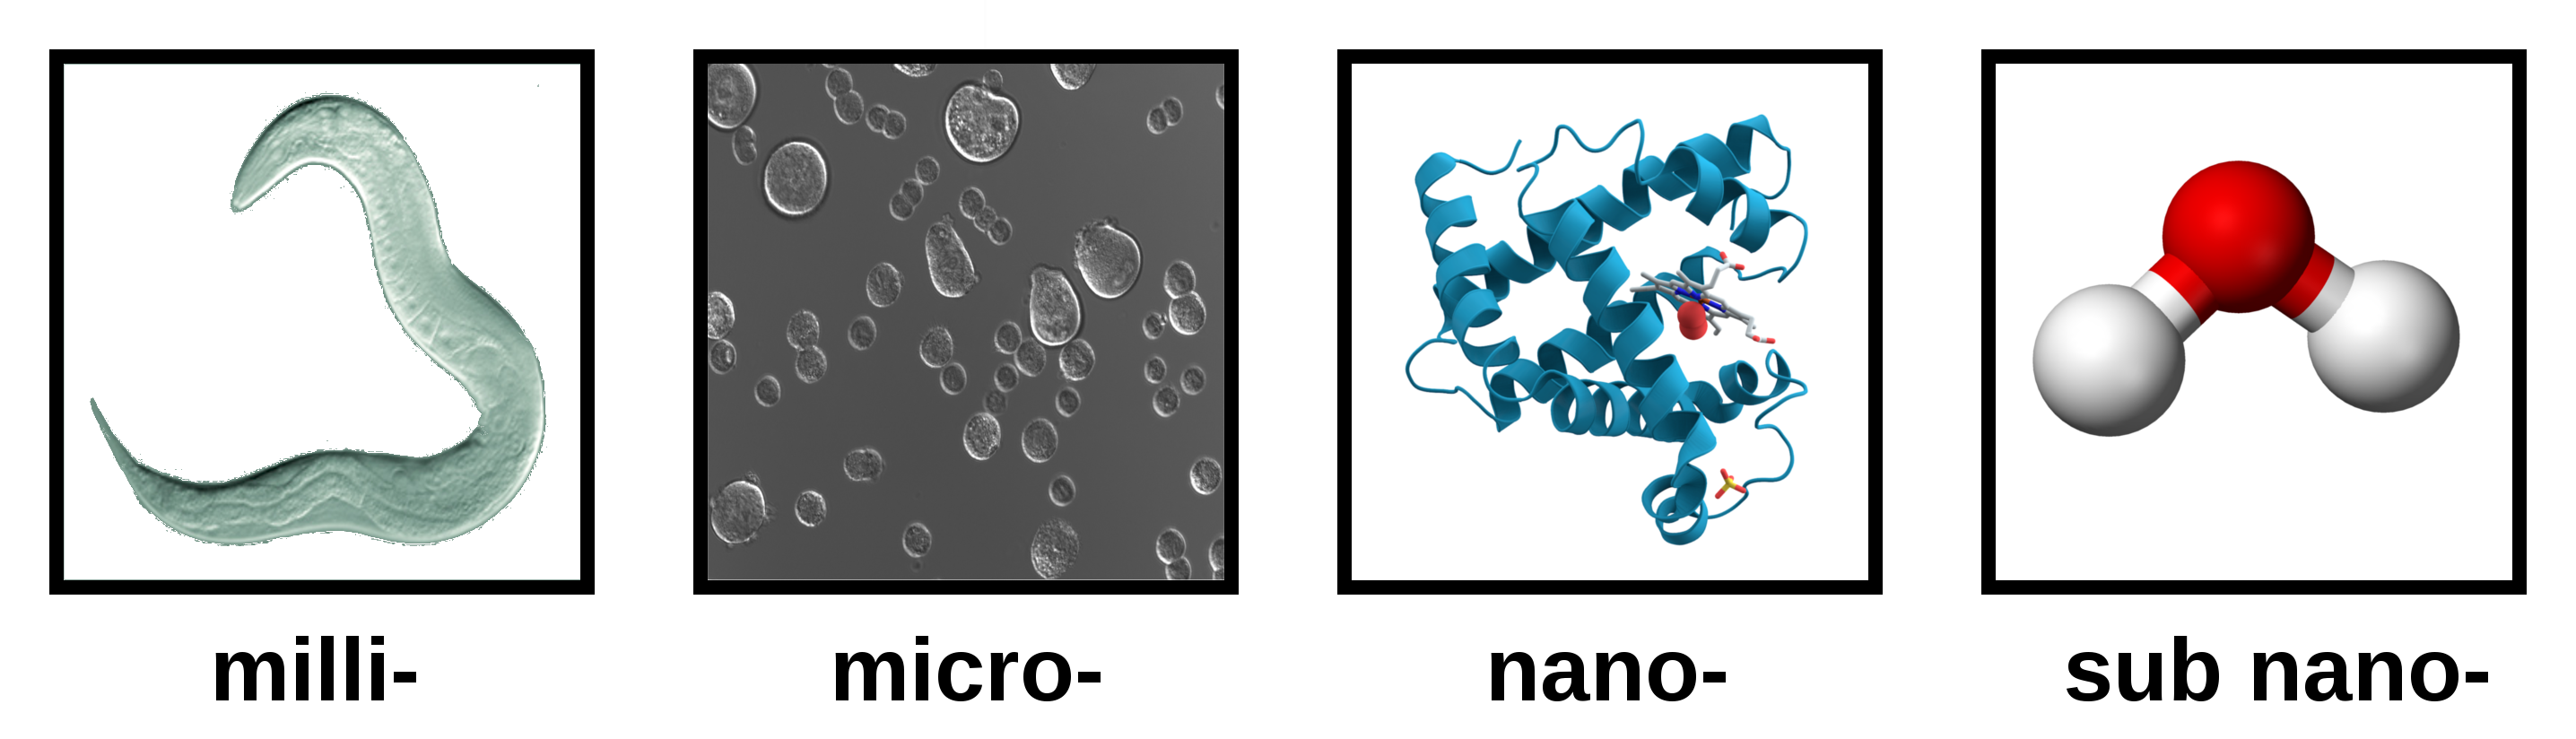
\includegraphics[width=\textwidth]{scales.png}
			\caption{Four important length scales for fluidics and surface forces. \textbf{milli-}: Caenorhabditis elegans (\textit{c. elegans}) sample, approximately 1 mm in length. Surface tension and capillary forces become significant at this length scale. Fluid dynamics is described by the complete Navier-Stokes equations. \textbf{micro-}: HCT-116 (colorectal cancer) cells, approximately $\SI{10}{\mu m}$ in diameter. Surface effects become increasingly important. Gravity becomes increasingly negligible, and systems under small applied pressures are described by having low-Reynolds number. \textbf{nano-}: A protein. Fluidic systems are dominated by surface forces. Liquid within $\SI{1}{nm}$ of surfaces is entirely contained within the electrical double layer. Fluid is completely non-inertial. \textbf{sub nano-}: A water molecule. Mean-field approximations are no longer valid. Navier-Stokes breaks down. Physics is determined entirely by electrostatic and Van der Waals forces between individual atoms and molecules.}
		\end{figure}
		
		\subsection{Pore/channel}
		
			The pore/channel itself is the primary actor of interest in our systems. The pore is created in some material, and the material properties as well as the fabrication procedure dictate the shape and geometry of the pore. As we will see, ionized chemical groups on the surface of the pore play as important a role as geometry in determining the behavior of the pore system.
		
		\subsection{Electrolyte solutions}
		
			Life on Earth exists in primary a \textit{fluid} environment, with the primary fluid being water. Water is the solvent for the chemistry of our bodies, and acts as the medium that allows electrolytes to ionize and transport between areas. In synthetic nanopore systems, we immerse our pore in an electrolyte solution that fills the channel, and under an applied voltage induces conduction of ions.
			
		\subsection{Electrodes}
		
			In order to create an external voltage in our system, an electronic voltage must be transformed into an ionic voltage potential. This is achieved \textit{via} ion electrodes, which allow transferrance of electrons into the ions of the solution and vice-versa, and the ions from the electrode then become the conductors in the system. This transferrance is known as a redox reaction in chemistry. For the rest of the thesis, unless specified we turn a blind eye to the chemical conversion process at the surface of the electrodes, and pretend that our electrodes are ideal voltage sources.
			
		\subsection{Particles}
		
			Because so many of the applications of interest for nanopore and microchannel studies involve biomolecule manipulation, we often work with electrolyte solutions that contain a suspension of particles in addition to the ions. The particles used are tied to the application, but often respond in the same way to forces present in teh system.

		\subsection{Equations of motion for fluidic systems---Navier--Stokes equations}
		
			One of the major actors in nanopores systems is the fluid solvent, which may remain at rest or, more commonly, move in response to forces present in the system. Because the motion of the solvent couples to the motion of other actors present in the system, understanding the physical laws governing the fluid medium is crucial. For systems large compared to the size of molecules, we make the approximation that the fluid is a continuous rather than discrete medium. In reality, we know that fluids are not continuous but ar emade up of discrete atoms and molecules, which may make this approximation seem limiting. However, the continuum approximation has been shown to accurately describe fluids all the way down to the scale of a single nanometer, and thus are valid in most systems of interest \cite{Bocquet2010}. Under the continuum approximation, the equations of motion of the fluid are described by the Navier-Stokes equation.
			
			The Navier-Stokes equations are actually three coupled 2nd order non-linear partial differential equations that yield the fluid vector velocity $\vec{u}$. Despite the apparent complexity of the equations, they can be derived simply using Newton's 2nd law $\frac{d\vec{p}}{dt}=\vec{F}$ and conservation principles.
			
			Consider an integrable quantity $\phi$ that is convected in a fluid field with velocity $\vec{u}$. For a given control volume, the continuity equation relates the time rate of change of $\phi$ in the volume with the flux through the boundaries due to convection in the fluid field and the of sources and sinks that create or consume the field. The continuity equation is 
			
			\[ \frac{d}{dt}\int_{V}\phi dV=-\int_{A}\phi\vec{u}\cdot\hat{n}dA-\int_{V}s dV, \]
			
			where $dV$ is the control volume, $dA$ its bounding surfaces, $\hat{n}$ the unit normal to the surface $dA$, and $s$ are the sources and sinks present in the control volume, with the convention that sinks are positive and sources negative.
			
			If we consider the quanity to be the max flux (the momentum density) $\phi=\rho \vec{u}$ and simplify the equation, we arrive at the Cauchy momentum equation:
			
			\begin{equation}  \label{eq:cauchymomentum}
				\begin{split}
					\rho\frac{\partial\vec{u}}{\partial t}+\rho\vec{u}\cdot\vec{\nabla}\vec{u} &= \vec{s} \\
					\rho\frac{D\vec{u}}{Dt} &= \vec{s}.
				\end{split}
			\end{equation}
			
			The derivative $\frac{D}{Dt}$ in the second term is the material derivative, which describes the time rate of change of the velocity of a fluid parcel given that its change is time and position-dependent. Written in this way, we see that the equation for momentum continuity in the fluid leads us to a Newton's second law type expression. The term $\rho\vec{u}\cdot\vec{\nabla}\vec{u}$ is known as the convective term, and describes the transport of momentum due to motion of the flow-field itself.
			
			Next, we replace the sources and sinks $\vec{s}$ with their physical origins. Because the quantity of interest is momentum, we recognize that the sources and sinks must be forces (force densities) in the system, which can generally be broken down into body forces, such as those due to electrostatics or gravity, and surface forces. Therefore, we replace the source/sink term with $\vec{s}=\vec{\nabla}\cdot\matr{\sigma}+\sum_{i}\vec{f}_{i}$, where $\matr{\sigma}$ is the Cauchy stress tensor and $\vec{f}_{i}$ is a body force acting on the control volume. We can further break down the Cauchy stress tensor into the sum of two separate pieces, an isotropic pressure tensor $p\matr{I}$ and the stress tensor $\matr{\tau}$ due to \textit{viscous} forces. For Newtonian fluids like water, there is a fundamental postulate that the stresses $\sigma$ are proportional to the strain rates, with proportionality constant $\eta$, the viscosity of the fluid. In this case, $\matr{\tau}=2\eta\matr{\epsilon}$, where $\epsilon$ is the strain rate tensor which describes the deformation of the fluid due to velocity gradients. When the stress tensor $\matr{\tau}$ is replaced with the strain rate tensor $\matr{\epsilon}$ via the constitutive relationship for Newtonian fluids, we finally arrive at the full Navier-Stokes equations:
			
			\begin{equation} \label{eq:ns}
				\rho\frac{\partial \vec{u}}{\partial t}+\rho\vec{u}\cdot\matr{\nabla}\vec{u}=-\matr{\nabla}p+\eta\matr{\nabla}^{2}\vec{u}+\sum_{i}\vec{f}_{i}.
			\end{equation}
			
			Solving the Navier-Stokes equation yields the correct fluid velocity $\vec{u}$ at all points in the system. While it is a complex equation, in many systems it can be simplified and solved analytically. For instance, in microfluidic channels gravity is often insignificant compared to other inertial and pressure forces, and is often ignored. Additionally, in small channels and with relatively small velocities, the inertial/convective term $\left(\vec{u}\cdot\nabla\right)\vec{u}$ is often negligible and can be dropped. To quantify this notion, we introduce a dimensionless parameter called the Reynolds number:
			
			\begin{equation} \label{eq:reynoldsnum}
				Re=\frac{\rho u L}{\eta}.
			\end{equation}
			
			$L$ in the above equation is the characteristic length scale of the flow, which in pores or channels is chosen to be the diameter by convention. The Reynolds number $Re$ is essentially a ratio of the strength of inertial/convective forces to inertial forces. For high Reynolds number, convective forces dominate and we expect turbulent and chaotic flow. At low Reynolds number, inertial forces dominate and fluid motion is laminar and smooth. The Reynolds number is useful for knowing which two regimes we are in, and can provide intuition about the behavior of our systems. In microfluidic systems, we are seldom in the turbulent regime, and are often at medium to low Reynolds numbers. Nanofluidic systems are almost certainly non-inertial for reasonable external pressures.
			

			
		\subsection{Motion of ions in a solvent---Poisson-Nernst-Planck equation}
		
			While the Navier-Stokes equations of motion describe the motion of the fluid solvent, the Poisson-Nernst-Planck, or PNP equations describe the motion (flux) of ions in the solution. The flux of ions is due to the superposition of diffusion, advection in the fluid solvent (known as `streaming' current), and migration in electric fields (e.g.~ due to external voltage sources). Summing the individual contributions, the PNP equation for the flux of an ion species is
			
			\begin{equation} \label{eq:pnp}
				\vec{J_{i}}=-\left[D_{i}\matr{\nabla}c_{i}-\vec{u}c_{i}+\frac{D_{i}z_{i}e}{k_{B}T}c_{i}\matr{\nabla}\phi\right],		
			\end{equation}
	
			where $\vec{J_{i}}$ is the ion flux of species $i$, $D$ is the diffusion coefficient, $c$ is the ion concentration, $z$ is the ion valence, $e$ is the elementary charge, $k_{B}$ is the Boltzmann constant, $T$ is the temperature, nad $\phi$ is the electric potential. The first term in eq. \ref{eq:pnp} is the diffusion term, which essentially states that there is a flux of ions in the opposite direction of the gradient of the ion concentration. The second term is the advective term, which accounts for the ions moving with the fluid solvent. The final term is the electric migration term, which describes the motion of the ions in an electric field gradient. 
			
			
			
			
		\subsection{The diffuse layer---Poisson-Boltzmann equation}
			
			The diffuse layer is of paramount importance in nanopore studies; without it, nanopores would simply act as passive conductors with no interesting conductance properties. When any type of material is submitted in solution, charges tend to appear at the surface. Some of these charges are due to specific adsorption or immobilization of ions or molecules onto the surface, which give the surface some charge. The other charge type which is usually more significant is due to the ionization of chemical groups native to the surface of the pore. The type of chemical group present on the pore depends on the material out of which the pore is made. For instance, polymer pores prepared via the track-etch technique are formed when an etchant solution cleaves the monomer units in half, exposing a carboxyl group, which is then deprotonated at basic solution pHs. On average there are approximately 1 of these surface groups per $\SI{4}{nm}^{2}$, yielding a net surface charge density of $0.25~\mathrm{e}/\mathrm{nm}^{2}$. In any case, the total charge that mobile ions `feel' in the solution is the sum of the adsorbed charges (Stern layer), plus the chemical groups attached to the surface, plus the immobilized ions within the slip layer. The electric potential immediately outside the Stern layer due to these superimposed charged sources is known as the $\zeta$ potential.
			
			
			
			\begin{figure}
				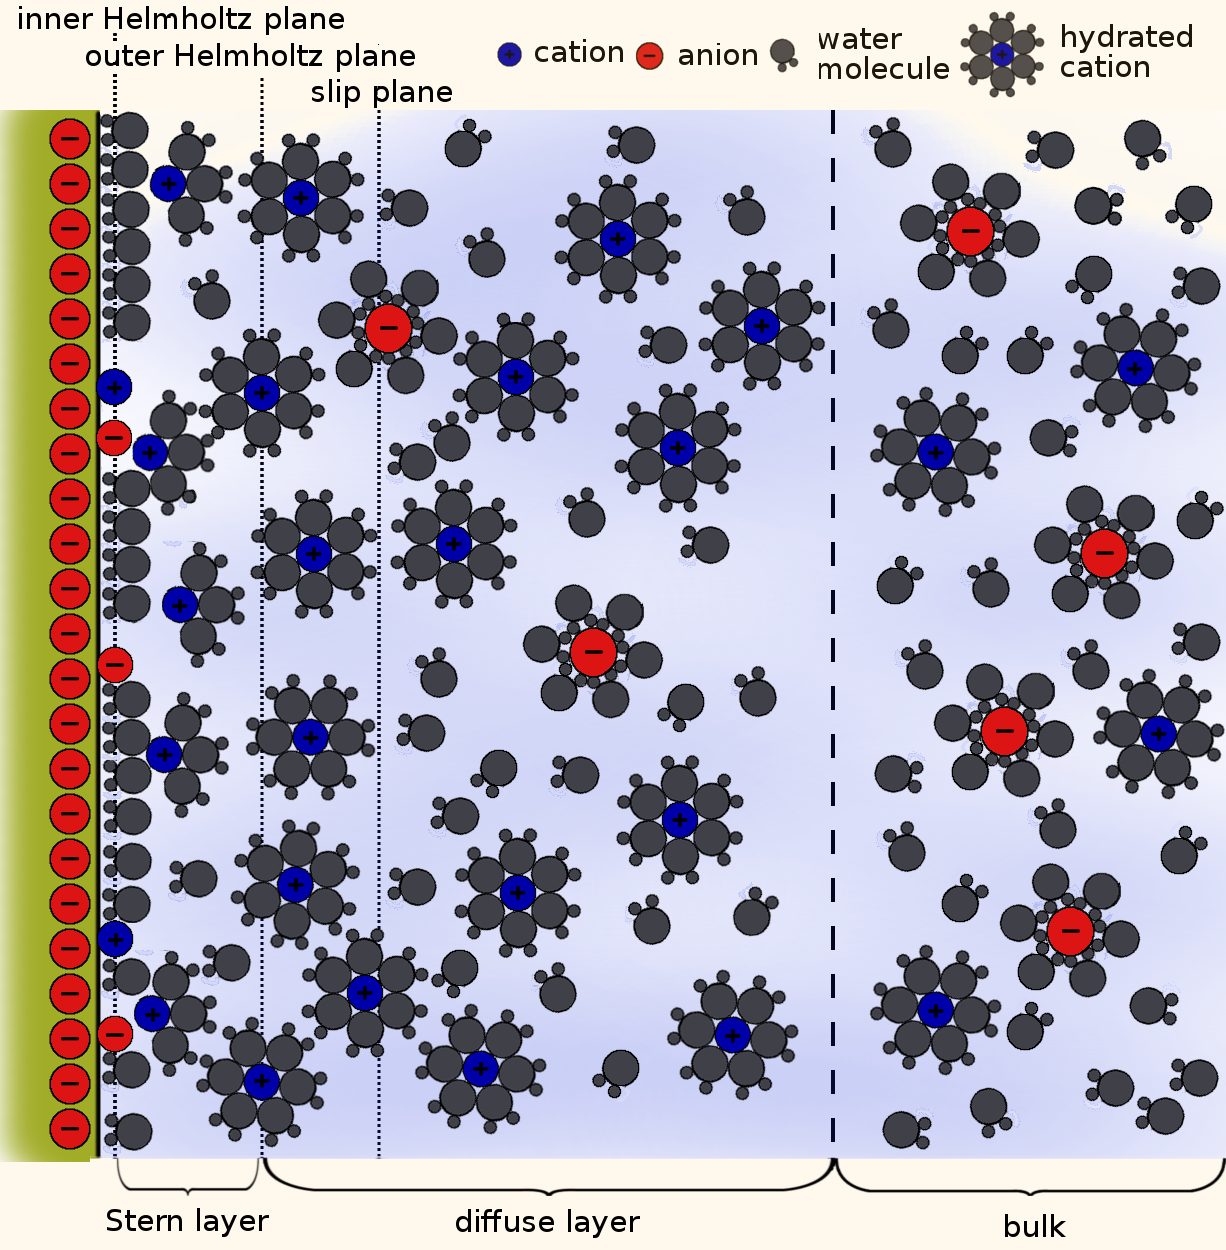
\includegraphics[width=\textwidth]{edl.png}
				\caption{Scheme of the electrical double layer under the Gouy-Chapman and Stern model. There is an abundance of counterions near the pore surface and a reduced number of coions. At the bulk both ion species' concentrations are equal.}
				
				 \label{fig:edl}
			\end{figure}
			
			Because the ion solution is conductive, mobile ions outside the Stern layer will redistribute themselves near the charged surface to counter or `screen' its $\zeta-$potential. This screening layer is known as the Debye layer, and is characterized by an enriched number of counterions (ions of opposite charge polarity to the wall) and a depleted number of coions. As we will see, the electrical double layer has a characteristic length scale known as the Debye length $\lambda_{D}$, which ranges from $0.1-10$ nm for most solution concentrations. Figure \ref{fig:edl} gives a view of the electrical double layer under the combined Gouy-Chapman and Stern models. 

			
			\begin{figure}
				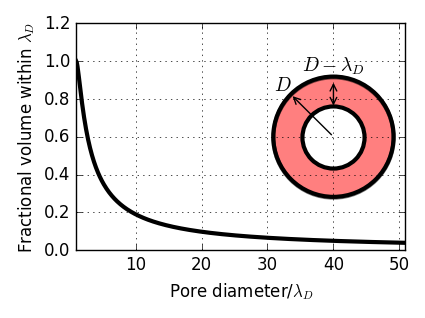
\includegraphics{fractioninsideedl.png}
				\caption{Plot of fraction of volume in a nanopore that is within the EDL versus pore diameter. The plot reveals a large super linear increase of total solution within the EDL as diameter decreases, starting at approximately $D\approx 10\lambda_{D}$.}
				
				\label{fig:fractioninsideedl}
			\end{figure}
			
			Nanopore's interesting behavior emerges when a non-negligible amount of the total volume is within a distance of $\lambda_{D}$ of the pore wall. Assuming $\lambda_{D}=1$, figure \ref{fig:fractioninsideedl} shows the fractional area of pore contained within $\lambda_{D}$ of the pore wall as a function of the pore diameter $D$. 
			
			
			
			For pores with diameter $D\gtrsim10\lambda_{D}$, the total volume within the electrical double layer is negligible; however, below approximately $10\lambda_{D}$ the total volume within the EDL quickly increases. This explains why the `nano' prefix in nanopore is important; as we approach the scale of the EDL, the structure of the solution very quickly changes, in a non-linear fashion, within the vicinity of a few nm of the pore wall.
			
			
			
			In order to derive the appearance of the EDL, we consider the equations governing the distribution of ions in solution. In the solution, the ion species $i$ have an electrostatic potential energy $U_{i}=z_{i}e\phi$, and have the following distribution in accordance with Boltzmann statistics
			
			
			
			\begin{equation} \label{eq:boltzmann}
				c_{i}=c_{0,i}\mathrm{e}^{-\frac{z_{i}e\phi}{k_{B}T}}.				
			\end{equation}
			
			The electric potential itself is given by the Poisson equation
			
			\begin{equation} \label{eq:poisson}
				\begin{split}
					\matr{\nabla}^{2}\phi & = -\frac{\rho}{\epsilon} \\
					\matr{\nabla}^{2}\phi & = -\frac{1}{\epsilon}\sum_{i}z_{i}ec_{i}\left(y\right).
				\end{split}
			\end{equation}
			
			Plugging the concentrations given by the Boltzmann equation into the Poisson equation, we arrive at the Poisson-Boltzmann equation
			
			\begin{equation} \label{eq:pb}
				\matr{\nabla}^{2}\phi=-\frac{1}{\epsilon}\sum_{i}z_{i}ec_{0,i}\mathrm{e}^{-\frac{z_{i}e\phi}{k_{B}T}}.
			\end{equation}
			
			The Poisson-Boltzmann equation \ref{eq:pb} is a second order non-linear differential equation for the electrostatic potential $\phi$; after solving for $\phi$, it can be plugged back into the Poisson equation \ref{eq:poisson} to obtain the ion concentrations $c_{i}$. The Poisson-Boltzmann equation is generally solved numerically, but analytic solutions exist for simplified assumptions about the geometry and magnitude of the electrostatic potential in the solution. 
			
			Consider a planar surface with unit normal pointing in the $\hat{y}-$ direction and uniform surface charge density $\sigma$ immersed in a solution of water and symmetric ions with molar concentration $c_{\pm}$, valency $z_{\pm}=z$, and identical diffusion coefficients $D_{i}$; this ion configuration is a close approximation of a KCl electrolyte solution, a common-used electrolyte in nanopore experiments due to the near-perfect symmetry of the ions. The ions have electrostatic potential energy given by $U_{i}=z_{i}\mathrm{e}\phi\left(y\right)$ where the electric potential $\phi$ is only a function of distance from the wall due to the system's symmetry. Under these assumptions, the Poisson-Boltzmann equation becomes
			
			\[ \frac{d^{2}\phi}{dy^{2}}=-\frac{zec_{0}}{\epsilon}. \]
			
			Though the solution can be solved analytically, a simple solution is obtained when we linearize the right hand side of the equation under the assumption $zec_{0}\ll k_{B}T$ and apply the correct boundary conditions, an approximation known as the Debye-H\u ckel approximation. The solution is
			
			\begin{equation} \label{eq:pb1d}
				\begin{split}
					\phi &= \phi_{0}\mathrm{e}^{-\frac{y}{\lambda_{D}}} \\
					c_{i} &= c_{i,0}\mathrm{e}^{-\frac{z_{i}e\phi_{0}}{k_{B}T}\mathrm{e}^{-y/\lambda_{D}}} \\
					\lambda_{D} &= \sqrt{\frac{\epsilon k_{B}T}{2c_{0}}}z,
				\end{split}				
			\end{equation}
			
			\begin{figure}
				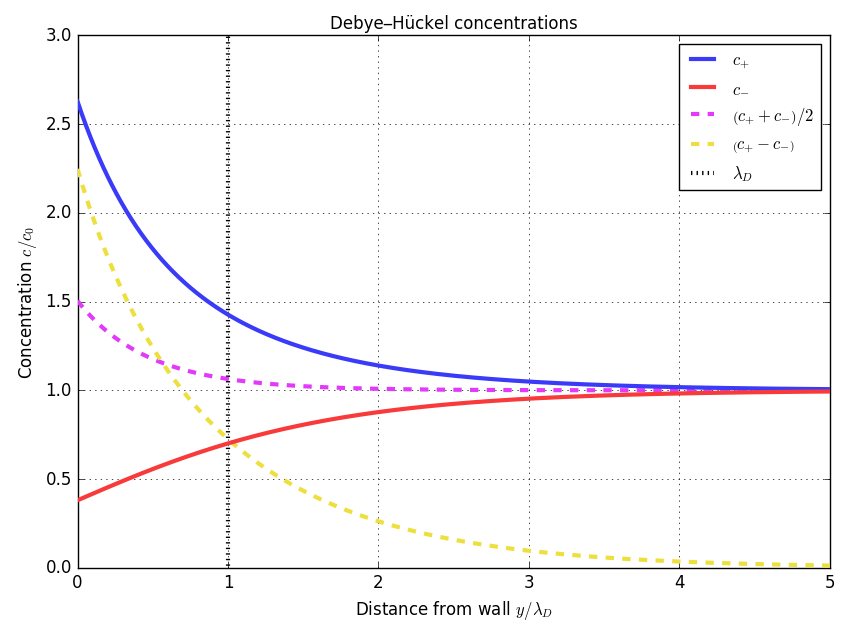
\includegraphics[width=\textwidth]{EDL_Charge_Distribution.png}
				\caption{\textbf{Ion concentrations adjacent to a negatively charged surface according to the Debye-Huckel theory.} The plot reveals that the counterion concentration (blue) is enhanced near the wall, and decays approximately exponentially as distance from the wall increases. Oppositely, coions (red) are diminished near the wall, and rise to their bulk value with distance from the wall. The \textit{total} ion concentration at the pore surface is slightly higher than the total ion concentration in the bulk. The space charge density $\rho_{E}\propto\left[c_{+}\left(y\right)-c_{-}\left(y\right)\right]$ is non-zero near the wall, and decays to zero in the bulk.}
				\label{fig:EDLChargeDistribution}
			\end{figure}

			
			where we introduced a new parameter, the Debye length $\lambda_{D}$. The solution to the 1-D lineared Poisson-Boltzmann equation reveals that the electrostatic potential exponentially approaches 0 from the wall, that the counterion species are enriched at the surface and diminish towards the bulk, and the coions are diminished at the surface, but recover their concentration towards the bulk. The Debye length is perhaps the most useful parameter in nanopore systems since it gives a characteristic length scale for the region within the pore wall that departs from its bulk, ordinary behavior. The Debye length increases with dilute ion concentrations and decreases as the ion concentration is increased, and is typically somewhere in the range of $0.1-10$ nm for common solution preparations. Note that although we discussed the electrical double layer here in the context of a pore surface, nearly every body immersed in solution will have some surface charge and therefore its own electrical double layer. The electrical double layers of free-bodies i.e.~particles are integral in explaining their motion in applied electrical fields, also known as electrophoresis. 
			
			The importance of the EDL in bestowing nanopores with their novel conductance properties cannot be overstated, and accordingly there are many phenomenon that nanopores that exhibit that are a direct consequence of the present of the EDL. In the next few sections we will review some of these phenomena.
			
			
		\subsection{Electroosmosis}
			
			Ions migrate in externally applied electric fields, and ions of opposite polarity travel in opposite directions. When ions move, they tend to drag fluid along with them. In the bulk, this fact results in no net motion of fluid because for every anion that drags fluid towards the cathode, there is a cation that drags fluid towards the anode, and the two motions cancel each other out so that there is no net motion of fluid. However, as we've just learned there \textit{is} a net concentration of one ion polarity in the EDL, so we expect that an electric field applied parallel to a charged surface will induce motion of the fluid. This intuition turns out to be correct, and the effect is known as electroosmosis. Interestingly, although the effect originates due to the presence of the $\sim \SI{1}{nm}-$thick EDL, the induced fluid flow propogates well into the bulk, and electroosmosis is observable in micro- and even milli-sized systems. This result, while surprising, is due to the simple viscous coupling of the fluid at the EDL surface to the rest of the fluid.
			
			Because electroosmosis induces a general fluid flow, the effect couples with the motion of all unbound actors in the system, namely the ions species and any particles suspended in the solution. In typical nanopores, convection in the electroosmotic flow tends to be less pronounced than migration in the electric field. However, some lightly charged particles for instance will only experience a small force from the electric field (electrophoresis) compared to the drag force from the fluid moving electroosmotically, and their motion is therefore determined primarily by electroosmosis. For the case of ions, usually the electroosmotic convective velocity adds or subtracts only a small offset to their net total motion, which remains dominated by electrophoresis. However, recently it was shown that some types of channels exhibit frictionless flow of water, and in these cases the electroosmotic velocities can become very large. In these channels it is actually expected that electroosmotic offers a large, if not dominant contribution to the motion of ions in the system. One example of these special types of pores, carbon nanotube pores, will be discussed later in this dissertation.
			
			To understand electroosmosis, we look to the Navier-Stokes equations which describe the motion of fluids, and the Poisson-Boltzmann equation which yields the distribution of ions in the vicinity of the EDL. As an example, consider again an infinite charged plane with unit normal pointing in the $\hat{y}-$ direction, but this time with a constant electric field $\vec{E}$ applied parallel to its surface. The Navier-Stokes equation (eq \ref{eq:ns}) simplifies greatly in this case, and simply becomes
			
			\[ 0 = \eta\frac{\partial^{2}u}{\partial y^{2}}+\left[c_{+}\left(y\right)-c_{-}\left(y\right)\right]zeE_{ext}. \]
			
			The equation shows that there is a momentum flux source term from the electric field acting on the charged solution in the EDL, which is proportional to the net charge in the solution (proportional to $c_{+}-c_{-}$) times the electric field $\vec{E}$. The other term that balances the driving force is due to viscous forces between neighboring layers that have different $y-$ velocities $u$, i.e. due to velocity gradients perpendicular to the wall. In order to solve this equation, we can replace the charge density $\rho_{E}=ze\left(c_{+}-c_{-}\right)$ with the Laplacian of the scalar potential $\phi$, integrate twice, and apply the correct boundary conditions, that the velocity at the pore wall is 0 (the so-called `non-slip' boundary condition) and that the velocity gradients are 0 infinitely far from the wall.  Performing these steps, we find the fluid velocity equals 
			
			\[ u=\frac{\epsilon E_{ext}}{\eta}\left(\phi-\zeta\right), \]
			
			where $\phi_{0}$ is the electric potential immediately outside the surface charges on the pore wall. Interestingly, according to this equation the fluid velocity is proportional to the local electric potential in the screening layer, which is determined by solving the Poisson-Boltzmann equation (Eq. \ref{eq:pb}). Under the Debye-H\u ckel approximation of small surface potentials, the fluid velocity is zero at the walls, and exponentially approaches its bulk value as distance from the wall increases. This type of fluid flow profile is known as `plug flow', since the velocity is approximately constant everywhere except in the thin EDL where there are sharp velocity gradients. Since the potential in the bulk is equal to $\phi=0$, we find the bulk velocity to be equal to 
			
			\begin{equation} \label{eq:hs}
				\begin{split}
					u &= -\frac{\epsilon\zeta}{\eta}E_{ext} \\
					u &= \mu_{EO}E_{ext},
				\end{split}
			\end{equation}
			
			

			
			a result known as the Helmholtz-Smoluchowski equation. The parameter $\mu_{EO}\equiv-\frac{\epsilon\zeta}{\eta}$ introduced is known as the electroosmotic mobility, and is the proportionality constant between the applied electrical field and the resulting fluid velocity. Typical values of the mobility are $\mu_{EO}=10^{-8} \left[m^{2}/V s\right]$, which for an electric field of $\SI{1}{V/\mu m^{2}}$ yields a fluid velocity of approximately $\SI{1}{cm/s}$. 
			
			\begin{figure}
				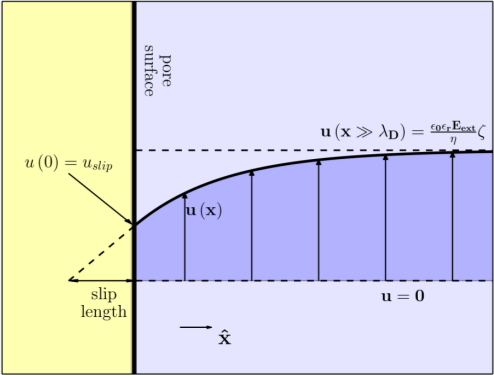
\includegraphics[width=.5\textwidth]{electroosmosis.png}
				\caption{\textbf{Plot of electroosmotic flow along an infinite plane with finite slip length}. A net ion charge at the surface experiences a force in an electric field which drags fluid along with it. The force is only present in the electrical double layer, which viscously couples to the rest of the fluid. This fluid flow profile is known as plug flow, and extends far beyond the EDL where it originates.}
				\label{fig:electroosmosis}
			\end{figure}
			
			Figure \ref{fig:electroosmosis} shows the fluid flow profile in a pore with a finite slip length $u_{\mathrm{slip}}$; however, it must be noted that in the vast majority of experimental systems, $u_{\mathrm{slip}}=0$.
			
			It is possible to experimentally observe the fluid flow velocity, for instance by tracking the motion of small particles that move in the fluid flow, and therefore Eq. \ref{eq:hs} provides a means for directly measuring the $\zeta-$potential.
			
		\subsection{Surface conductance and conductance saturation}
		
			\begin{figure} 
				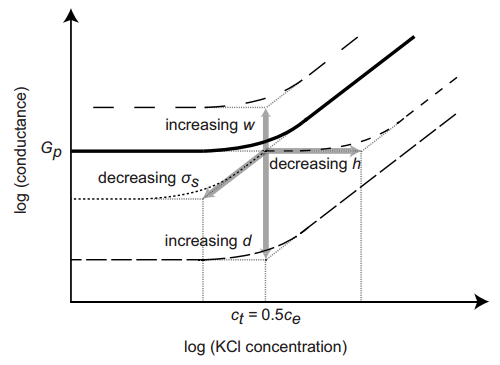
\includegraphics[width=0.5\textwidth]{Schoch2008_conductance}
				\caption{Reprinted (abstract/excerpt/figure) with permission from [(FULL REFERENCE CITATION) as follows: Author's Names, APS Journal Title, Volume Number, Page Number and Year of Publication.] Copyright (YEAR) by the American Physical Society.}
				\label{fig:Schoch2008conductance}
			\end{figure}
		
			Ignoring electrical double layer effects, the conductance of an ion channel is proportional to the ion concentration in the solution; doubling the ion concentration exactly doubles the measured current. However, the presence of the electrical double layer breaks this perfect linear conductance relationship for two reasons. First, the integrated \textit{excess} ion count $\int_{0}^{EDL}=\left[\left(c_{+}+c_{-}\right)-2c_{0}\right]dy$ in the EDL layer is not guaranteed to be the same as the total ion concentration in the bulk; in fact, in most cases it is slightly higher, meaning the electrophoretic current in the EDL is slightly higher than in the bulk. Another important contribution to the measured current is the current from convection due to electroosmosis; because there is a net charge density in the fluid, electroosmosis will create a measurable ion current! In total, there are three terms that contribute to the total current measured in a channel, migration of ions in the bulk, migration of the integrated ion \textit{excess} in the EDL, and net convection of charge in the EDL due to electroosmosis. Without applying any equations, we can use what we learned about the EDL and some general logic to reason about what the current behavior should be in the limiting cases of very large ion concentration and very small ion concentration. The equation for the Debye-length is $\lambda_{D}\propto c_{0}^{-1/2}$; for very large ion concentration, the EDL should be negligible and therefore neither the effects of electroosmosis nor electrophoretic ion excess should be significant. At the other end of the scale, in the limit of nearly zero ions in the bulk we still must have charge neutrality in the pore, meaning a finite concentration of ions despite the bulk concentration being zero. In this case, the EDL fills the entire pore and the result is that the conductance is entirely due to the integrated excess and convective terms. This finite conductance at zero concentration is known as the \textit{saturation current}. Therefore, as we increase the length of the EDL we expect the conductance discrepancy, the difference in bulk conductance versus conductance due to the two surface effects, to increase. The end result of all this is that the conductance is a non-linear function of ion concentration at sufficiently low ion concentration; removing ions past some point does not further reduce the conductance of the channel! Consider a nanopore immersed in solution of two symmetric ions denoted $+$ and $-$ (symmetric means their mobilities, valencies, and bulk concentrations are equal) with electrophoretic mobility $\mu_{EP}$ and electroosmotic mobility $\mu_{EP}$. The following expression breaks down the total measured current into the three components described above:
		
			
			\begin{equation} \label{eq:totalconductance}
				\begin{split}
					I &= I_{\mathrm{bulk}}+I_{\mathrm{excess}}+I_{\mathrm{EO}} \\
					I &= \int 2c_{0}\mu_{EP}EezdA + \int\left[c_{+}\left(z\right)+c_{-}\left(z\right)-2c_{0}\right]\mu_{EP}EezdA + \int\left[c_{+}\left(z\right)-c_{-}\left(z\right)\right]u_{\mathrm{EO}}\left(z\right)ezdA.
				\end{split}
			\end{equation}
			
			Figure \ref{fig:Schoch2008conductance} shows a plot of the conductance versus solution concentration for a nanopore; the plot reveals a saturation at low solution concentration as expected from the preceding arguments. The saturation current is equal to the surface conductance term in the above equation.
			
		\subsection{Ion selectivity}
			A phenomenon related to surface conductance is \textit{ion selectivity}. Since the EDL has a higher concentration of counterions rather than coions, the total flux of ions through the pore is slightly skewed towards counterions. The ion selectivity is defined as
			
			\begin{equation} \label{eq:selectivity}
				S=\frac{|I_{+}-I_{-}|}{I}.				
			\end{equation}
			
		
		\subsection{Ionic current rectification}
			An ion channel is said to be rectifying if its conductance for one voltage polarity is greater than the opposite voltage polarity. The presence of an EDL alone cannot account for this, since the system has symmetry with respect to switching the electrodes, and therefore no rectification will occur. However, by introducing asymmetry into a system, along with having the pore be partially ion selective, we can create rectifying pores. There are many ways to create asymmetric nanopores, but two obvious solutions are geometry and surface charge pattern based.
			
			If the shape of a nanopore is asymmetric, for instance as in a cone, the ionic current will be rectified. A simple explanation for this is that at the tip-side of the pore (in the case of conical nanopores), there will be an excess of counterions in the vicinity of the entrance EDL, while the other side will more closely resemble the bulk. Because these ions are at the entrance of the pore, they will more easily enter the pore than when at the other side. The result is that for one voltage polarity the ionic current is greater than at the opposite polarity.
			
			By similar reasoning, charge patterning asymmetry can also lead to rectification. By placing two charges of opposite polarity adjacent to one another inside the pore, for one voltage polarity a depletion zone is created in analogy with the depletion zone formed between the n- and p-doped regions in a semiconductor diode. The ionic current is rectified, and because the diode junction so severely limits the ionic current under one voltage polarity, the device is said to be equivalent to an ionic diode.\cite{Vlassiouk2007}
			
			\begin{figure}
				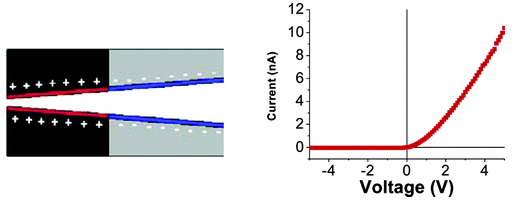
\includegraphics[width=.5\textwidth]{Vlassiouk2007_conicaldiode}
				\caption{\textbf{An ionic diode formed in a conical nanopore with bipolar surface charge patterning.} The region between negative and positive charges is the depletion zone, and provides a large resistance to ion flow through the pore for one voltage polarity. Reprinted with permission from \bibentry{Vlassiouk2007}. Copyright 2007 American Chemical Society.}
				\label{fig:Vlassiouk2007conicaldiode}
			\end{figure}
			
			Figure \ref{fig:Vlassiouk2007conicaldiode} shows a conical nanopore with a bipolar charge distribution. The combination of the geometrical and charge asymmetry gives the pore a very large rectification value, and the near-zero current for one polarity of voltage is enough to consider the pore a diode.

			
			


			
			
		
			
			
		
			
			

			
			
		\subsubsection{Particle electrophoresis}
			
			Electrophoresis is the transport of a charged particle in the presence of an electric field. The effect of electrophoresis can be derived much in the way electroosmosis was derived, but instead of considering the fluid flow velocity at the surface of the particle to be zero, we set it equal to the electrophoretic velocity. For particles with thin electrical double layers (Debye-H\u ckel approximation) and laminar flow (Stoke's flow), the particle velocity is
			
			\begin{equation} \label{eq:electrophoresis}
				\begin{split}
					\vec{u} &= \frac{\epsilon\vec{E}_{0}}{\eta}\phi_{0} \\
					\vec{u} &= \mu_{\mathrm{EP}}=\frac{\epsilon\phi_{0}}{\eta}.
				\end{split}
			\end{equation}
			
			In equation \ref{eq:electrophoresis}, we've again introduced a proportionality factor between the applied electric field $E_{0}$ and the induced velocity $\vec{u}$; this factor is known as the electrophoretic mobility. However, these equations are derived under the assumption that the applied electric field does not perturb the distribution of ions in the electrical double layer, which is only true for small surface potentials. If this assumption is invalid, additional effects related to the redistribution of ions must be taken into account; the net effect is a retarding force on the particle that slows its velocity.
			
			Electrophoresis is an important effect in many applications involving particles. One useful application is that particle electrophoresis through a nanopore can be used to measure the zeta potential of a particle, related to its surface chemistry and chemical adsorption. An electric field is applied across a nanopore which is immersed in electrolyte solution containing ions and charged particles. Particles travel through the pore under electrophoresis, and the dwell time can be recorded using resistive pulse sensing or optical techniques. If the geometry of the pore is known, the dwell time can be related with the particle velocity, and the electric field strength can be determined as well. In this case, equation \ref{eq:electrophoresis} can be solved for the surface potential $\phi_{0}$, which is the same as its zeta-potential.
			
		\subsubsection{Particle electrophoresis + electroosmosis}
			Transport of particles is in general a superposition of electrophoretic and electroosmotic effects. Combining the two, the velocity of a charged particle translocating through a charged pore is 
			
			\begin{equation} \label{eq:particlevelocity}
				\begin{split}
					v=\left(\mu_{EP}+\mu_{EO}\right)E, \\
					v=\frac{\epsilon}{\eta}\left(\zeta_{\mathrm{particle}}-\zeta_{\mathrm{pore}}\right)E
				\end{split}
			\end{equation}
			
			In general the net velocity can be positive, negative, or zero depending on the relative sizes and signs of the electrophoretic mobility.



			

			
			
			

			
			
			
			

			
			


			
	





%%% Local Variables: ***
%%% mode: latex ***
%%% TeX-master: "thesis.tex" ***
%%% End: ***

\graphicspath{{../images/ch2/}}	% Image directory


\chapter{Development and testing of a single carbon nanotube based pore}

	

	\section{Background}
	
		This chapter describes my research performed on measuring the ion, water, and particle transport properties of single carbon nanotubes. A carbon nanotube (CNT) is a cylindrically-shaped monolayer of carbon atoms, and because of its shape it can effectively act as a nanopore.  When used as nanopores, CNTs are thought to exhibit behavior that is significantly different than traditional nanopores, including large fluxes of water, large fluxes of some ion species, steric rejection of other ion species, ultra-high proton mobilities, and an unusual sub-linear power law in the conductance-concentration relationship. These effects are poorly understood, and since it was discovered that they could be used as single nanopores many labs around the world have worked on understanding them. Besides being poorly understood, there is even a lack of consensus in the field about whether some of these properties are even real! The objective of this experiment was to test a new CNT platform that could help point the field in the right direction; by observing transport phenomena in our CNT platform, hopefully we nudged the field in the direction of a concensus. 
		
		In the following sections, I will explain in greater depth a functional CNT nanopore platform, and the physical reasons underlying their novel transport characteristics.
		
		
		
	

	




%%% Local Variables: ***
%%% mode: latex ***
%%% TeX-master: "thesis.tex" ***
%%% End: ***

\graphicspath{{../images/ch3/}}	% Image directory


\chapter{Experimental study of ion conductance property of hybrid conductor-insulator nanopores}

	

	\section{Background}
	
		In the introduction of this thesis we discussed the electrical double layer (EDL) which is a screening layer of ions that forms in the proximity of a charged surface. The vast majority of pores studied are non-conductive insulators, and their surface charge properties come from the functionalization of chemical groups at their surface. For instance, the base of the pore studied in this section is $\mathrm{Si{3}N_{4}}$ (silicon nitride), whose native silane chemistry means there are exposed alcohols at the surface that are either negative or neutral depending on pH. However, charge on a surface can arise \textit{via} other means. When a metal is exposed to an electric field, electrons in the metal rapidly redistribute themselves on the surface to cancel the external applied field. If we assume the metal was originally overall neutral, the charge pattern will consist of an abundance of negatively-charged electrons at one end and an abundance of positively-charged holes at the other. A natural question is whether these \textit{induced} charges have associated EDLs in the same way that static charges do.
		
		Previous studies suggest they do. For instance, Squires \textit{et al.} and Pascall \textit{et al.} performed experiments with applied external electric fields on various metal surfaces and discovered that electroosmotic flow occurred. They reasoned that electroosmosis was a result of polarization of charges according to the model discussed above \cite{Squires2004, Pascall2010}. However, these types of induced-charges have been seldom discussed in hte context of nanopore transport, especially in the context of an realizable experimental platform. In order to understand the effect of induced charges on nanopore transport, we considered a hybrid metal-insulator pore created by evaporating a thin layer of gold onto the pore surface. If the pore was only the insulator, its IV curve would be symmetrical due to the lack of any symmetry breaking in the system. The addition of the metallic layer breaks this symmetry, and we expect to see ionic current rectification in the pore (see chapter 1.) However, ionic current rectification alone is insufficient for proving that induced surface charges contribute to the pore's conductance; this is because essentially \textit{any} symmetry breaking in a pore, including a difference in static surface charges between two regions, a difference in geometrical shape between two regions, \textit{or} induced surface charges, will lead to ionic current rectification.
		
		\begin{figure}
			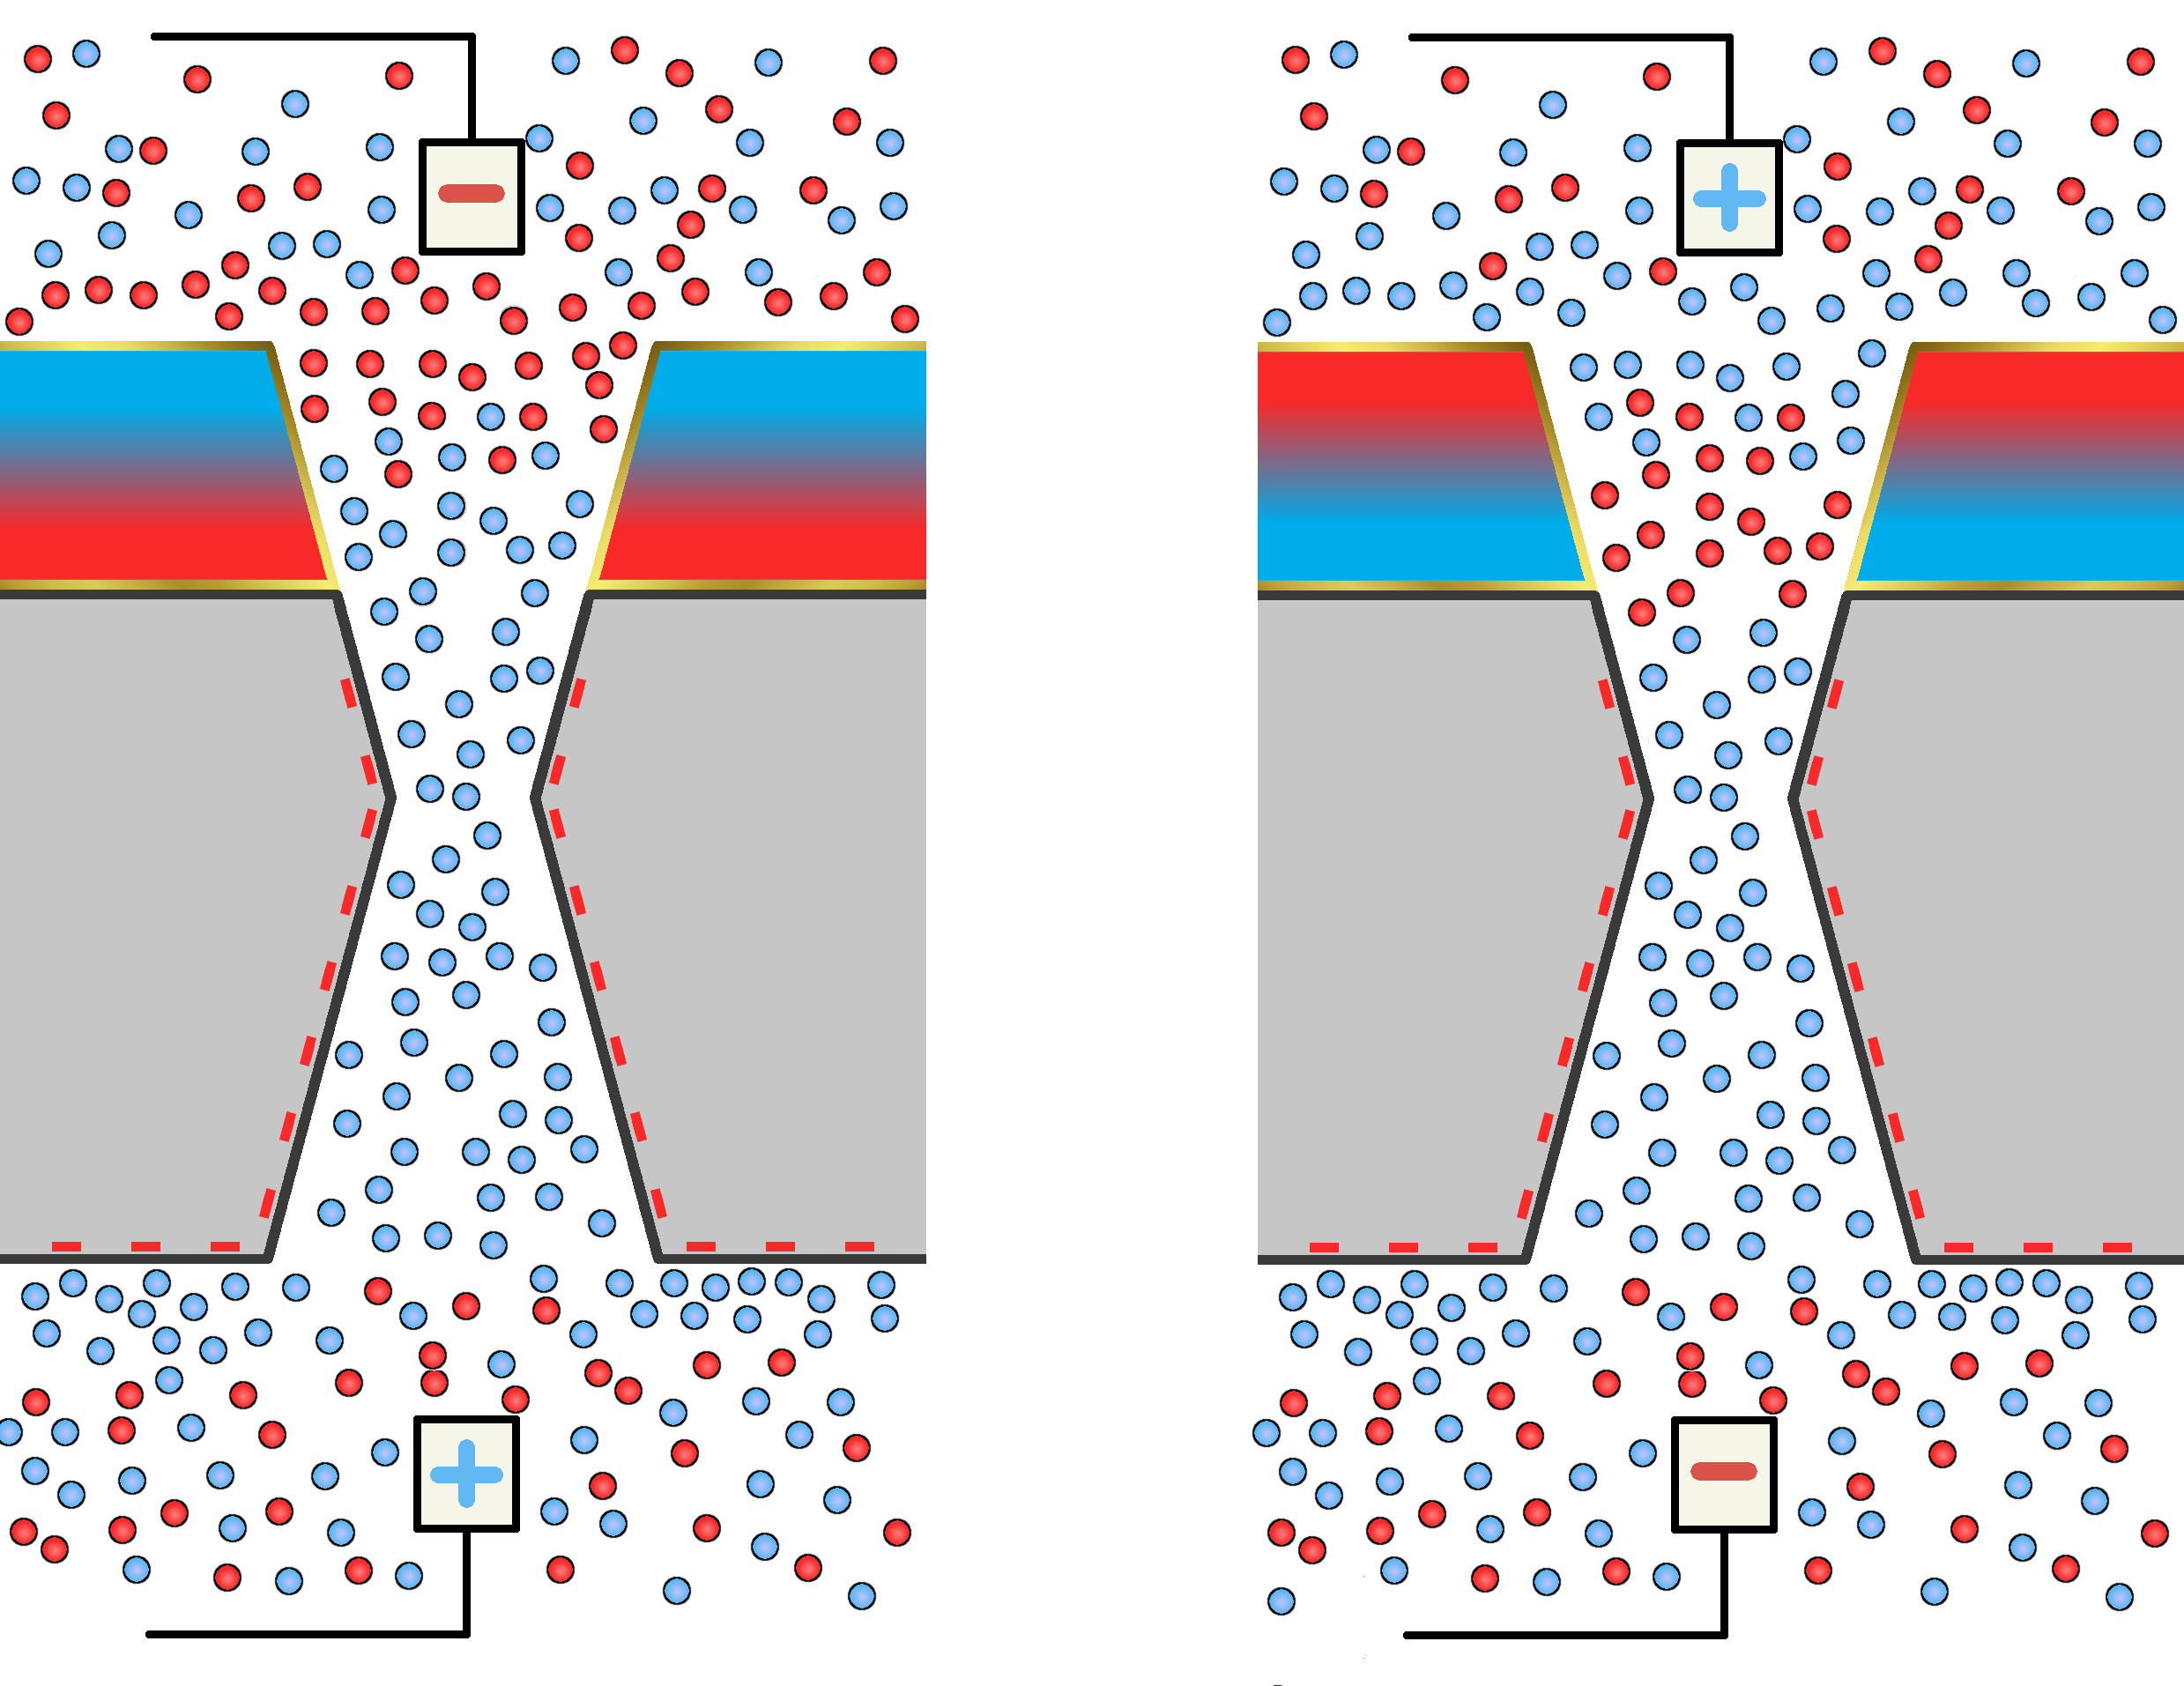
\includegraphics[width=0.5\textwidth]{SiN-Gold_Model.png}
			\caption{\textbf{Model for the induced-charge and EDL charges in the hybrid conductor-insulator nanopore.} \textbf{Left:} Negative bias applied to gold side. \textbf{Right:} Positive bias applied to gold side. For the positive bias, a depletion zone forms at the junction between the gold and SiN, which is expected to severely limit the conductance. For the negative bias, no depletion zone forms and therefore the conductance is expected to be unhindered. The double conical geometry reflects the expected geometry of SiN pores drilled \textit{via} a transmission electron microscope electron beam.}
			\label{fig:SiNGoldModel}
		\end{figure}

		
		In order to provide evidence that induced charges directly contributed to a pore's conductance properties in this system, we need to devise a model for the manner of the induced rectification properties, and to check if the model accurately describes experimental data. Figure \ref{fig:SiNGoldModel} is a scheme of the induced-charge model, which is effectively explained by the surface charges present. First, the insulating part of the pore has an approximately uniform surface charge due to ionization of the chemical groups on its surface. On the gold, the charge patterning depends on the applied voltage. When a negative bias is applied on the gold side of the pore, electrons are repelled from the electrode while holes are attracted. The charge pattern in the solution from top to bottom is then $-++$. On the other hand, when a positive bias is applied on the gold-side of the pore, holes flee to the inside of the pore while electrons are drawn towards the electron. Therefore, from the positive electrode to the negative electrode the surface charge pattern is $+-+$ (right hand side of figure \ref{fig:SiNGoldModel}. The primary difference in the charge pattern as it relates to the influence on the nanopore between the two voltage polarity cases is the charge juntion at the conductor-insulator interface; in the latter case (positive voltage applied on the metallic side), the $+-$ junction indicates the presence of a bipolar junction that leads to a depletion zone in the EDL, as discussed in the section on ionic current rectification in chapter 1. This depletion zone is characterized by having a very large resistance, and therefore limits the total current through the pore. For the opposite polarity, the depletion zone is not present and therefore we do not expect any significant limiting of the current.
		
		This model, known as the induced-charge model for hybrid conductor-insulator nanopores, was tested experimentally in this work.
		
	\section{Experimental setup}
		
		In order to test the induced-charge model, we devised a platform consisting of thin nanopores in silicon nitride (SiN) with gold (Au) deposited on top. The crucial elements of this setup consisted of the silicon nitride (SiN) membrane, evaporated gold (Au) layer, transmission electron microscope drilling of the pore, and the current-voltage characterization measurements.
		
		\subsection{Silicon nitride}
			
			Silicon nitride was used as the substrate through which to drill the nanopore. The effects of polarization of the gold should be apparent in truly nano-scale systems, so it was important to choose a material through which a small pore could be fabricated. As of the writing of this thesis, silicon nitride (chemical formula $\mathrm{Si_{3}N_{4}}$) is a popular choice for creating small nanopores given its mechanical stability and well-understood surface chemistry. The method of pore formation, TEM drilling (discussed below) can enable pores ranging from $1-20$ nm in diameter, and is capable of drilling through substrate lengths of up to $100$ nm. It is predicted that pores with very low aspect ratios, i.e.~short pores, will have severely diminished rectification propeties. In order to ensure large rectification, the solution must be subjected to a sufficient length of EDL. In order to strike a compromise between TEM's capabilities and the undesirable low-aspect ratio effects, a substrate thickness of $\SI{50}{nm}$ was chosen. The silicon nitride substrate is commonly used in TEM microscopy, and therefore is available from commercial vendors. The substates were ordered from the SPI company. The substrate itself is grown onto a thicker layer of silicon, through which a window is drilled on the backside to expose the silicon nitride. The final result is a $\SI{50}{nm}$ thick layer of SiN supported by a silicon chip. After pore fabrication, silanol groups native to the pore surface act as surface charges if immersed in solution with pH beyond their pKa value of 
			
		\subsection{Gold deposition}
			
			Although the model of induced-charge rectification described above is independent of the type of conductor used, we chose to use gold (Au) because of its mechanical stability after deposition and its resistance to corrosion and oxidation, which could create a surface chemistry effect that could potentially obscure the relationship with the induced surface charges. With the conductor's material chosen, we think about the desired deposition thickness. In the model of induced-charge rectification described above, it is necessary to have a bipolar junction far enough inside the pore that a depletion layer can form. For this reason, we aimed to deposit a $\SI{30}{nm}$ layer of gold onto the surface of the SiN. There are a number of means of depositing metals onto surfaces, but given the thinness of the desired layer we chose to deposit \textit{via} an e-beam evaporation. During e-beam evaporation, a chunk of metal is pumped down in vaccuum and bombarded with high-energy electrons. The combination of low-pressure and large temperature caused by the bombardment with the electrons causes individual metal atoms to evaporate from the surface of the chunk along straight-line or ray paths. The atoms then hit the surface of the substrate, which is suspended above it, and stick. Although Au \textit{can} be deposited directly onto the surface of SiN, a thin layer ($\SI{3}{nm}$) of chromium (Cr) was first evaporated, which facilitates adhesion of the Au.
			
		\subsection{Transmission electron microscope drilling}
		
			\begin{figure}
				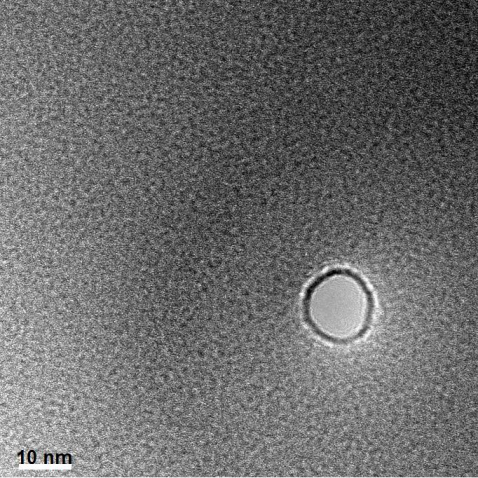
\includegraphics[width=0.5\textwidth]{sinpore.png}
				\caption{\textbf{A $\sim\SI{15}{nm}$ SiN pore drilled \textit{via} TEM.}}
				\label{fig:sinpore}
			\end{figure}

		
			The transmission electron microscope (TEM) is a super resolution imaging technique that is typically used to image objects below the optical diffraction limit of $\SI{200}{nm}$. However, if the electron beam is sufficiently energized and focused, the electron beam can act as a drill for forming nanopores instead of for imaging. This technique was used to drill pores through the SiN-Au hybrid device described in the above two steps. A highly focused beam in the TEM's scanning (S) mode is applied to the surface. The energetic electrons strike the surface and eject atoms, while simultaneously the entire structure melts. The final result is a pore with the same thickness as the substrate, and with a double conical geometry which is a result of the simultaneous ballastic ejection and melting. Because the drilling is performed inside the TEM, the resulting pore can also be immediately imaged. Figure \ref{fig:sinpore} shows an example of a $\sim\SI{15}{nm}$ TEM-drilled pore.
			
		\subsection{Pore conductance characterization}
		
			\begin{figure}
				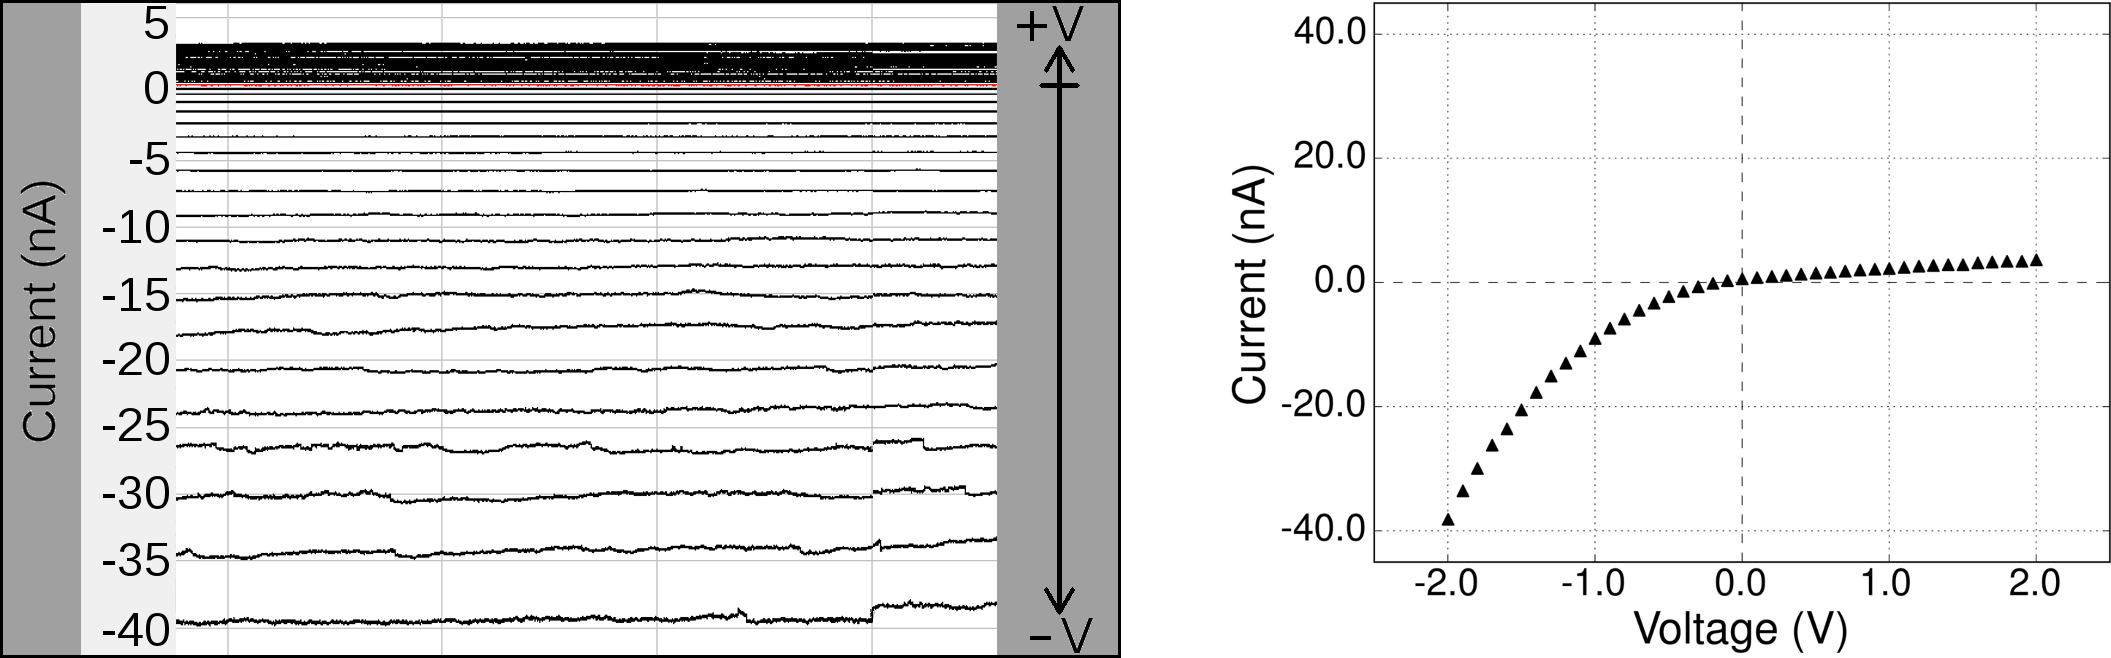
\includegraphics[width=\textwidth]{siniv.png}
				\caption{\textbf{A current-voltage time series alongside the current-voltage curve produced from it.} \textbf{Left}: Current-voltage time series. Each continuous line corresponds to one voltage setting; once a voltage value is set, the current does not significantly vary. \textbf{Right}: Traditional pore I-V curve. The asymmetry in the current with respect to voltage (present in both signals) is the hallmark indicator of ionic current rectification.}
				\label{fig:siniv}
			\end{figure}

		
			In order to test the induced-charge model, we measured the current-voltage (IV) response of each of the fabricated nanopores in $100$ and $500$ mM KF and KCl salt solutions. The total surface charge of a pore `felt' by the ions in the solution is given by a combination of the ionized chemical groups on its surface and any chemical species that are adsorbed to the surface. Cl is known to adsorb to the surface of gold, and so we expect that the gold in KCl solutions will have net charge given by the adsorbed chloride ions and the induced-charges. For this reason, measurements were performed primarily with KF solution. However, it was predicted that adsorption of chloride on the Au surface would diminish the effects of the induced-charge, and this model was tested by performing measurements with KCl on chips that had already been measured in KF, to see if their conductance behavior changed according to this prescription. 
			
			Due to the small sizes of the pore and the low surface charge density of the silanols on the SiN surface, the interior of the pore is difficult to wet, meaning any vapor present inside the pore can be stable and difficult to remove. If this is the case, ions cannot pass through. Often times these vapor phases are quasi-stableand the pore will spontaneously wet and dewet. In order to reduce these hydrophobic effects, we use an even 50/50 mixture of water and ethanol solvent; the combination of both solvents promotes wetting of the pore. 
			
			In principle, during IV measurements one needs only to sweep the voltage along the desired range, stopping to record the current at each voltage value. Usually one delays $\sim\SI{1}{second}$ after changing the voltage before a current measurement is made to allow for the system to equilibrate, e.g.~due to system capacitance charging/discharging. However, in systems in which the system conductance can stochastically change, e.g.~due to spontaneous wetting/dewetting transitions, it is advantageous to record a time series of the current voltage sweeps rather than measure single data points. If a transition occurs, it can be observed in the time series of the signal and appropriately dealt with afterwards. The protocol for measuring IV curves is then to apply a fixed voltage, record the current for a fixed amount of time, and repeat for all of the desired voltages. Then, an IV curve is produced by averaging the current time-series for a fixed interval of time (averaging is performed to smooth over the small amount of noise in the signal). In this study, voltages were applied for a total of $\SI{20}{s}$ and the current values in the last $\SI{0.5}{s}$ were averaged to create the current measurement value. Figure \ref{fig:siniv} shows an example current-voltage time series and the IV curve produced from it for one of the pores used in the study measured in KF solution. On the left is a current-voltage time series plot that shows the current value time series for different voltage settings, while the right hand side of the figure shows a traditional I-V curve of the pore.  
			
			
	\section{Experimental results}
	
		A number of conductor-insulator pores were tested, along with plain SiN pores to test of the pores intrinsically rectify the current (e.g.~due to a geometrical asymmetry).
		
		\begin{figure}
			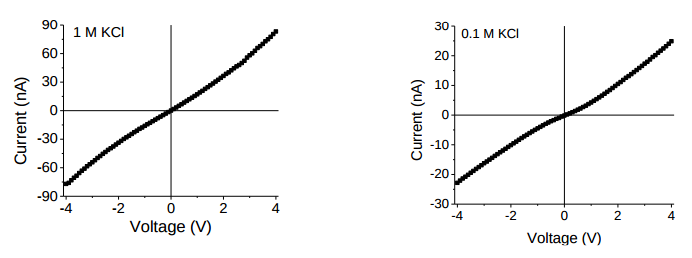
\includegraphics[width=\textwidth]{sinsymm}
			\caption{\textbf{IV curves taken of bare SiN pores}. The symmetry in the IV curve reveals no inherent rectification of the TEM drilled pores.}
			\label{fig:sinsymm}
		\end{figure}
		
		\begin{figure}
			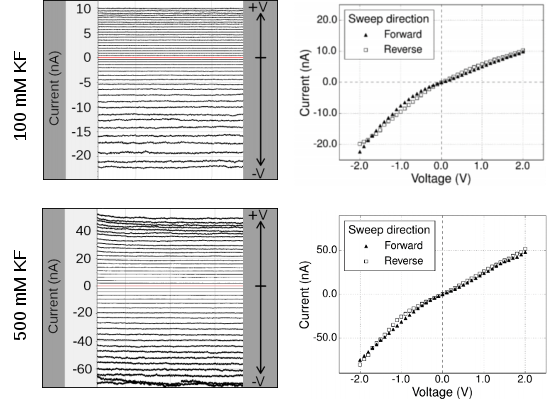
\includegraphics[width=\textwidth]{sinau0}
			\caption{\textbf{IV curves taken of Au-SiN pore in $\SI{100}{mM}$ and $\SI{500}{mM}$ KF.} The symmetry in the IV curve reveals no inherent rectification of the TEM drilled pores. The ion rectification ratio $R$ is lower in the higher concentration solution, as is expected from basic considerations of EDL thickness.}
			\label{fig:sinau0}
		\end{figure}
		
		\begin{figure}
			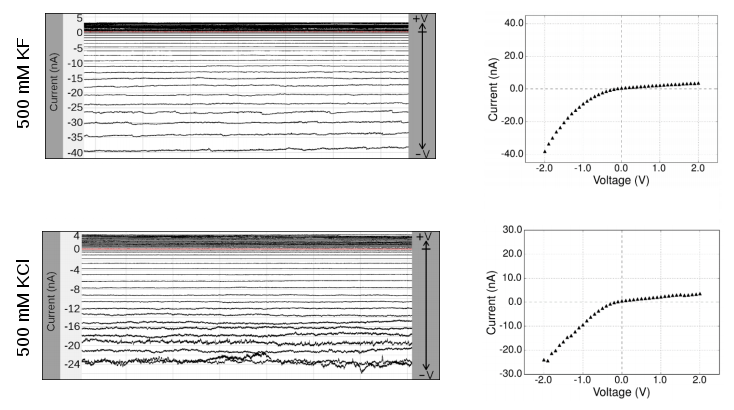
\includegraphics[width=\textwidth]{sinau1}
			\caption{\textbf{IV curves taken of Au-SiN pore in $\SI{500}{mM}$ KCl and KF.} The rectification ratio $R$ is lower in the KCl solution than in the KF solution, which is expected due to the additional contribution of the static charge from adsorbed $\mathrm{Cl^{-}}$ ions on the gold surface.}
			\label{fig:sinau1}
		\end{figure}


		
		Figure \ref{fig:sinsymm} shows two IV curves gathered for the SiN-only (insulator pore only). The plot shows approximately symmetric IV curves, indicating a symmetric nanopore. 
		
		On the other hand, figure \ref{fig:sinau0} shows two IV curves collected for a single nanopore approximately $\SI{9}{nm}$ in diameter. The IV curves taken in KF show significant rectification, with a ratio of approximately $R=0.5$ for the $\SI{100}{mM}$ concentration and $R=0.7$ for the $\SI{500}{mM}$ KF concentration. The increase in rectification $R$ towards $R=1$ with increasing salt concentration is consistent with the decrease in thickness of the EDL. In the model we developed for the induced-charge rectification, a depletion region is expected to form in the interior of the pore. Typically pores that have depletion zones experience much greater rectifications due to the `off-state' voltage polarity having nearly zero conductance. While this pore's rectification is not small enough (e.g.~not close to zero) to describe it as an ionic diode, the rectification direction is nevertheless consistent with the proposed model. We note that this direction of rectification is inconsistent with models having only static charges on the SiN and Au, barring the case where the $Au$ has positive charges adsorbed onto its surface, which is unexpected for the ion species used in this study.
		
		In order to understand the effect of a static charge superimposed on top of the induced-charge, we next performed experiments in KCl in addition to KF. Figure \ref{fig:sinau1} shows a $\SI{12}{nm}$ pore with IV curves measured in $\SI{500}{mM}$ concentration of both types of salts. Note that both salts give the same type of rectification as in the previous example. This result is not entirely unexpected, as the presence of adsorbed chloride will bring the two charges in the depletion zone closer together in magnitude, while still maintaining a finite, albeit reduced rectification. If the $Cl^{-}$ ions adsorbed to the surface of the gold to the extent that they dominated both the induced-charge on the gold and the surface charge on the SiN, then it is possible the rectification direction could even flip direction such that $R>1$. However, we did not observe such an effect.
		
	\section{Modelling results}
		
		In order to corroborate the lines of evidence pointing to induced-charge based ion current rectification found in experiments, we performed finite-element analysis simulations using the COMSOL Multiphysics software package. The models were designed to emulate the experimental set up, e.g.~the channel geometries and salt concentrations used were similar. However, rather than try to reproduce the double conical geometry expected for TEM drilled pores, we worked with a cylindrical geometry which greatly facilitated convergence of the solutions with the very minor penalty of not adhering exactly to the experimental conditions. Because the cone angle is expected to be shallow and because the COMSOL results are meant to be interpreted semi-quantitatively, and are primarily used to draw conclusions about the rectification direction and mechanism, replicating the exact geometry of the pore was deemed unneccessary.
		
		
			
			
		
			
		
			
	
		
		
		
		
	

	




%%% Local Variables: ***
%%% mode: latex ***
%%% TeX-master: "thesis.tex" ***
%%% End: ***

\graphicspath{{../images/ch4/}}	% Image directory


\chapter{Resistive pulse studies of aspherical mesoparticles}

	

	\section{Background \& Theory}
		In the introduction of this dissertation we introduced and explained the theory behind resistive pulse sensing, a particle characterization technique that works by monitoring the change in conductance of a nanopore as small particles pass through it. Probably the most important application of RP sensing is in measuring the sizes of particles. An analytic model was devised by DeBlois \emph{et al.} to relate the size of a particle to its resistive pulse amplitude. The solution is essentially an electrostatics boundary-value problem: given an insulating particle inside a pore and a known externally applied voltage, calculate the electric field distribution inside the pore, and from the electric field distribution calculate the pore's expected resistance with the particle inside it. When this calculation is performed for spherical particles travelling along the axis of long cylindrical pores, the change in resistance or current is found to be
		
		\begin{equation}\label{eq:dI}
			\frac{\Delta R}{R_{0}}=\frac{\Delta I}{I_{p}}=\frac{4\rho D^{3}}{\pi d^{4}}\left[1-0.8\left(\frac{d}{D}\right)^{3}\right].
		\end{equation}
		
		Equation \ref{eq:dI} is useful for relating the change in current---or resistance---to the diameter of spherical particles. However, it is very often the case that particles of interest are not spherical. For instance, many biomolecules such as viruses and proteins are poorly approximated as spheres, and are more rod-like in shape. In this case, the resistive pulse amplitude of on-axis translocations through a cylindrical pore is given by 
		
		\begin{equation}\label{eq:dIellipsoid}
			\frac{\Delta R}{R_{0}}=\left[f_{\perp}+\left(f_{\parallel}-f_{\perp}\cos^{2}\alpha\right)\right]\frac{v}{V},
		\end{equation}

		where $f_{\perp}$ and $f_{\parallel}$ are so called `shape-factors', that depend on the particle's major and minor axis lengths, $\alpha$ is the orientation of the particle with $\alpha=0$ being axially aligned, and $v$ and $V$ are the volume of the particle and of the pore, respectively. Figure \ref{fig:dIellipsoid} shows a plot of the relative $\Delta I/I_{p}$ for various ellipsoids of the same volume but different axial lengths.
		
		\begin{figure}
			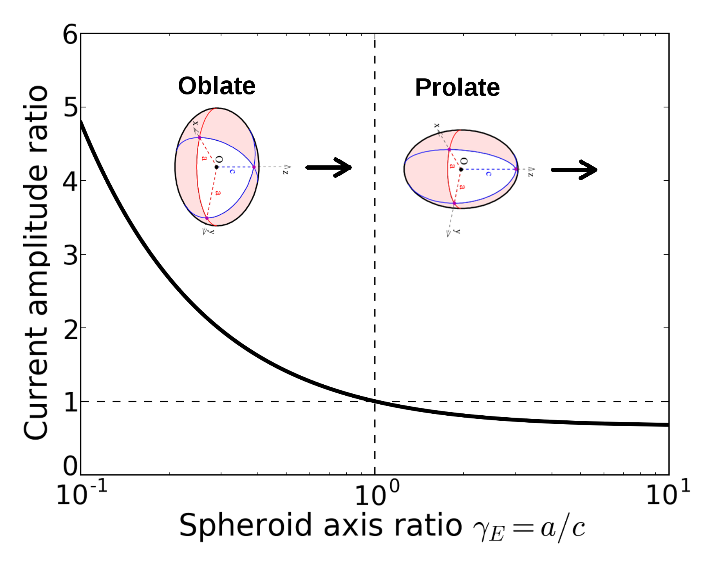
\includegraphics[width=0.5\textwidth]{dIellipsoid}
			\caption{adsf}
			\label{fig:dIellipsoid}
		\end{figure}

		
		
		
		
		
		
		While equation \ref{eq:dIellipsoid} is useful for determining the volume of spheroidal particles from their resistive pulse amplitudes, it would be useful to devise a method for measuring the length of particles in addition to measuring their volumes as an additional physical marker for their identification in a sample.
		
		Consider a pore with a rough, non-uniform interior. Due to the irregular interior, the channel cross sections will have a range of resistance values; for instance, a large cavity in the channel will have a smaller resistance than a more narrow constriction. If a very small particle travels through the pore, its resistive pulse time-series is determined by the interior topology of the pore. For instance, when it happens to occupy a narrower region of the pore, the resistance in tha tregion is larger relative to the rest of the pore, and therefore the particle  will also block a relatively larger portion of the current. In this way, the particle is able to resolve the interior features of the pore. In such cases, the instantaneous resistive pulse amplitude is given by 
		
		\begin{equation}\label{eq:dIlocal}
			\Delta R=R_{p}-R_{0}=\frac{4\rho d^{3}}{\pi D^{4}}\left[1-0.8\left(\frac{d}{D}\right)^{3}\right]^{-1}.
		\end{equation}

		
		\begin{equation}\label{eq:theoreticalmovingaverage}
			\Delta R=\Delta R'=\int_{z=z'}^{z=z'+l}R\left(z\right)=\int_{z=z'}^{z=z'+l}\frac{4\rho d^{3}}{\pi D^{4}}\left[1-0.8\left(\frac{d}{D}\right)^{3}\right]^{-1}
		\end{equation}

		
		Oppositely, if we consider a pore whose length extends along a significant amount of the pore's axis, it may be occupying several such regions at a time. Instead of a single particle, we may consider the particle to be composed of many smaller segments of particles in series, and therefore the resistance values of each segment are additive. Therefore, the signals of longer particles can be seen as the convolution of the signal of an infinitesimally small particle over the long particle's length. 
		
		This fact can be used to devise an experiment that can measure the length of long particles. First, we drive a suspension of small `tracer' spheres through a pore with rough interior, whose diameter is smaller than the characteristic length of the irregularities in the pore. These particles will `map' the interior geometry of the pore as explained above, with resistive pulse shape given by equation \ref{eq:dIlocal}. Then, we repeat the experiment with long particles for which we wish to know the length. Then we perform a convolution or moving average of the signals of the tracer particles for a variety of lengths; finally, a similarity measure is calculated between every pair of convoluted-raw signals for the tracer particle and the long particle, and the length with the greatest similarity measure is chosen as the correct length of the particle. 
		
	\section{Experiment}
	    
		\begin{figure}
			\hfill
			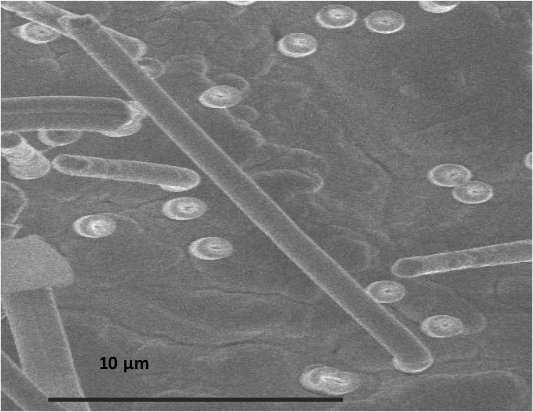
\includegraphics[height=0.35\textwidth]{PC}
			\hfill
			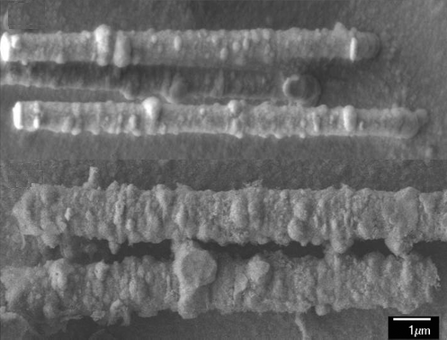
\includegraphics[height=0.35\textwidth]{PET}
			\hfill
			\caption{\textbf{Scanning electron microscope images of metal replica of track-etched PC (left) and PET (right) pores.} The pores were filled with metal and the polymer was completely etched a way, leaving a metal structure that is the inverse image of the pore. The metal was imaged in a scanning electron microscope. While the PC pores are nearly perfectly cylindrical in shape, the PET pores are characterized by rough inhomogenities across their entire surface, punctuated with large local bumps. The large bumps in the images of the metal replicas correspond to equally large cavitities in the PET pore.}
			\label{fig:PCPET}
		\end{figure}
		
		\begin{figure}
			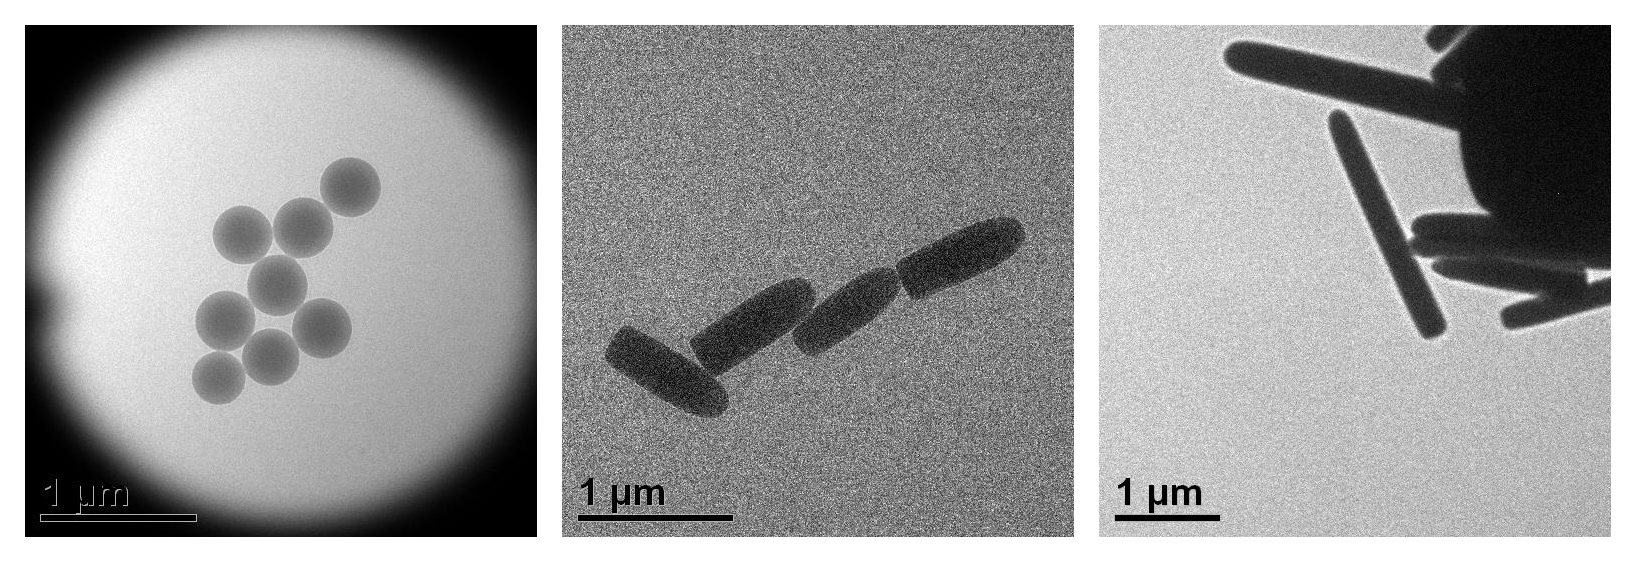
\includegraphics[width=1\textwidth]{particles}
			\caption{\textbf{Transmission electron microscope images of polystyrene beads and silica nanorods.} While the polystyrene beads are nearly perfectly spherical, the silica nanorods are approximately `bullet shaped'. For the purposes of this work, we approximated their shapes as ellipsoids in order to apply equation \ref{eq:dIellipsoid}.}
			\label{fig:particles}
		\end{figure}


	    
		In order to test the principle described above, we performed resistive pulse experiments with single mesopores ranging from $800-\SI{1000}{nm}$ in diameter. The materials used were polyethylene terephthalate (PET), a polymer which is known to have highly irregularly shaped interiors when pores are prepared \textit{via} the track-etch technique, and polycarbonate (PC), another polymer but with no axial inhomogeneities which will act as a control for the method. Figure \ref{fig:PCPET} shows images of both of these types of pores. For the particles, $\SI{280}{nm}$ and $\SI{410}{nm}$ in diameter polystyrene beads (`spheres') were used as the tracer particle, and rods of length $\SI{590}{nm}$, diameter $\SI{210}{nm}$ (`short rods') and $\SI{1920}{nm}$, diameter $\SI{240}{nm}$ (`long rods') were used to test the length measurement protocol; the particles are shown in figure \ref{fig:particles}. Particles were suspended in $\SI{100}{mM}$ KCl solution with $0.5\%$ Tween 80, a surfactant which prevents particle aggregation. The solution was then injected into both sides of a conductivity cell, and a voltage was applied across the pore. The resulting ionic current was sampled at $\SI{10}{kHz}$ and recorded. The polystyrene spheres used had a larger $\zeta-\mathrm{potential}$ than the pore, and therefore they translocated through the pore electrophoretically. On the other hand, the rods had a lower magnitude $\zeta-\mathrm{potential}$ than the pore, and therefore travelled through the pore under electroosmotic convective forces. 
		
	
	\section{Analysis \& Discussion}
	
	
		\begin{figure}
			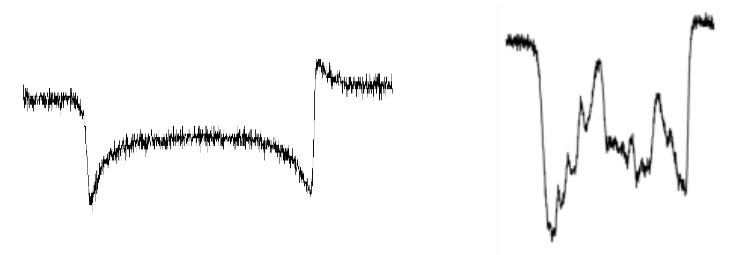
\includegraphics[width=0.5\textwidth]{PCPETevents}
			\caption{\textbf{Resistive pulse events through PC (left) and PET (right) pores.} As expected, the PET events are highly irregular and reflect the interior irregularities of the PET pore itself. On the other hand, the PC pores show no such irregularity. The events show that PC pores have large resistances at the beginning and end, reflecting the narrow, `pinched' diameters at the openings of the pores.}
			\label{fig:PCPETevents}
		\end{figure}

	
	
		Events were extracted from the current time series and studied separately; figure \ref{fig:PCPETevents} shows two events, one from a PC pore and one from a PET pore that are representative of the translocations through each type of pore. In the initial analysis, we looked at the average $\Delta I/I_{p}$ of the beads and rods and compared with the theoretical predictions of Eqs. \ref{eq:dI} and \ref{eq:dIellipsoid}. Figure \ref{fig:dIexp} shows the results for two pores, one $\SI{770}{nm}$ and another $\SI{1200}{nm}$ in diameter. For the two spheres studied, the measured $\Delta I/I_{p}$ was very close to the theoretical prediction (Eq. \ref{eq:dI}). The theoretical predictions were also very close to the measured values for the long rods. However, for both pores the theoretical prediction of the resistive pulse amplitude $\Delta I/I_{p}$ is far off for the short rods: the data shows a nearly 100\% discrepancy, i.e.~ the measured $\Delta I/I_{p}$ is nearly twice its expected value. This significant of a discrepancy is highly unusual, and one of the goals in the paper was to determine its cause. The discrepancy is made even stranger by the fact that the short and long rods are made of the same material, so any material contribution to the discrepancy e.g.~due to large $\zeta-\mathrm{potentials}$ is unlikely. Instead, we hypothesize that this discrepancy is due to their rotational dynamics. Equation \ref{eq:dIellipsoid} predicts that a prolate spheroid (like the rods) will have a larger $\Delta I/I_{p}$ when they are oriented with an off-axis component, but only considers static positioning. A very large rotational speed of the rods could couple to the measured $\Delta I/I_{p}$ amplitude in ways not captured by the equation, for instance by stirring the local solution in such a manner to reduce the local ion mobility. Furthermore, this hypothesis is consistent with the non-observance of the increased $\Delta I/I_{p}$ for the long rods, since at their length of $\sim\SI{1920}{nm}$ they are too large to rotate in even the larger of the two pores ($\SI{1200}{nm}$ in diameter). In any case, the net result is a measured volume for these particles that is approximately $2\times$ larger than their actual volume, which was confirmed with a combination of transmission electron microscopy images and dynamic light scattering. 
		
		The question, however, is how such a large rotation could occur. To answer this question, forces that cause rotation must be considered. In terms of translation (transport), the contributing forces are convection due to electroosmosis, and electrophoresis, as well as passive transport due to diffusion. Similarly, these forces could also contribute to rotational motion of the particles. The estimated rotational diffusion contribution of these rod particles is estimated as $13$ and $\SI{0.8}{rad/s}$ for the short and long rods, respectively. In order for fluid motion to cause rotation, it is necessary to have a non-constant fluid velocity profile on the pore's length. However, because the fluid velocity is due to electroosmosis there will be a nearly constant fluid velocity profile in the pore, which is unlikely to cause significant rotation. On the other hand, the rough undulations in the pore could create axial variations in the electric field; such variations could also lead to a net torque on the particle that causes rotation. In order to estimate the potential magnitude of the rotational velocities of the rods, we considered a simple model where the pore's diameter discontinuously changes from $\SI{1000}{nm}$ to $\SI{1100}{nm}$, a reasonable approximation for the geometries present in our system based on the images of the pores (see Fig. \ref{fig:PET}). Under this model, we calculate the electric field amplitude to differ by a factor of $1.2$ between the two regions. Using the rotational diffusion coefficient of the rods and integrating the electric field differences along the length of the pore, we calculate the angular rotation rate $\omega$ to be $\omega\sim10^{4}$ rad/s. Due to the preceding arguments, it is clear that the largest contribution to the rotation of the rods is from the electric forces. We believe that such a large rotation could make the rods behave as if they are much larger particles.
		
		\begin{figure}
			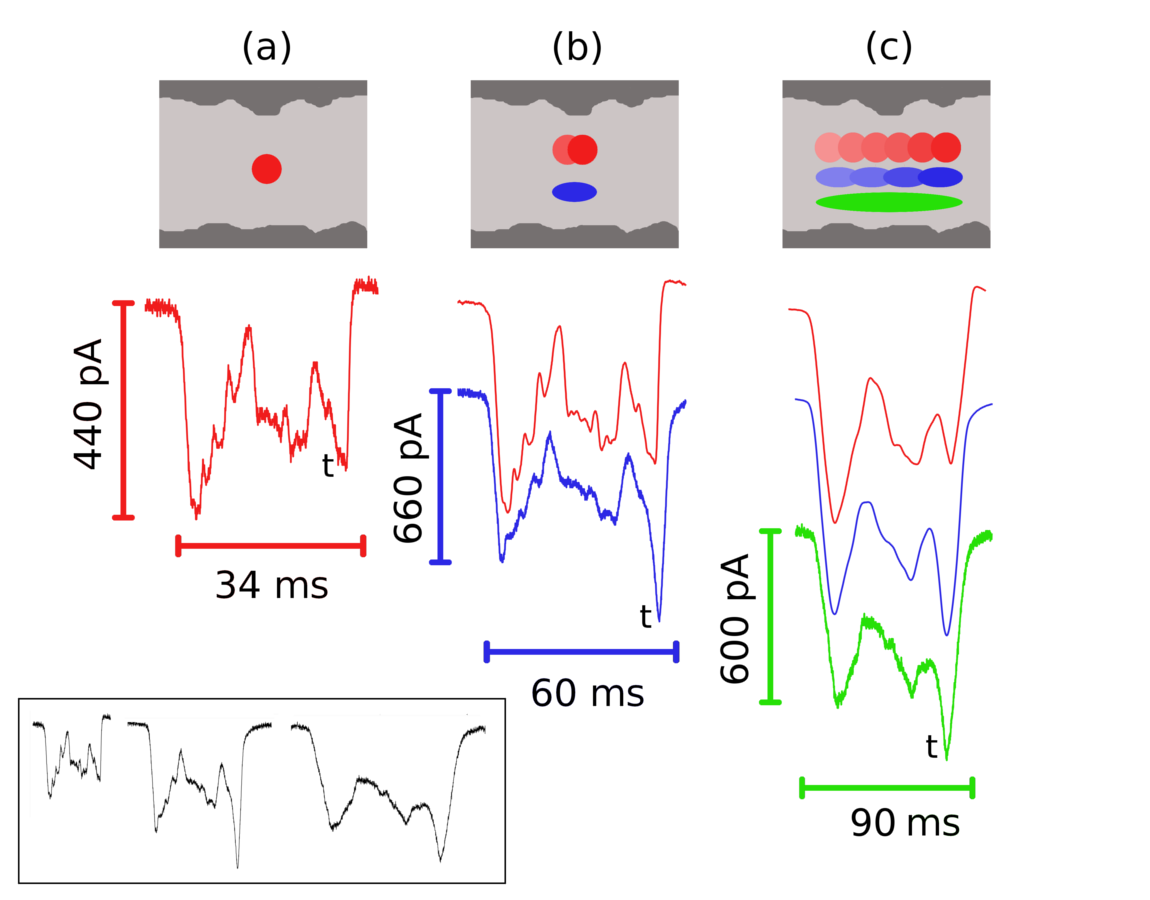
\includegraphics[width=.5\textwidth]{PETevents}
			\caption{\textbf{Resistive pulse events of a $\SI{410}{nm}$ diameter sphere (red), and $\SI{590}{nm}$ (blue) and $\SI{1920}{nm}$ (green) in length rods.} The top row shows a cartoon scheme of the pore with the particles inside its interior. The bottom resistive pulse event in each column corresponds to the raw recorded data; events above this are smoothed \textit{via} the moving average transformation. The bottom left figure shows the raw events on the same scale.}
			\label{fig:PETevents}
		\end{figure}

		
		Figure \ref{fig:PETevents} shows example recorded events for the three types of particles used in this study. A $\SI{410}{nm}$ sphere translocation is shown on the left column in red. Notice the roughness in the event; this roughness has been shown to correspond to the interior irregularities in the pore. Local $\Delta I/I_{p}\left(t\right)$ are large at relatively constricted points, and small at larger cavitated points. The green event in the right column corresponds to the raw resistive pulse signal of a long rod. Notice the difference in structure of the two events; the long rod's event shows some structure, but is missing many of the local minima and maxima that are present in the signal of the short rod. This observation is in agreement with our previous arguments for the smoothing of the pore interior that takes place for long particles. Without making any quantitative arguments, we are able to conclude that the particle corresponding to the green event is longer than the particle corresponding to the red event. In between those two extremes are the short rods in red. The short rods at length $\SI{590}{nm}$ are slightly longer than the spheres which have diameter $\SI{410}{nm}$, but due to their rotation it is not entirely obvious whether they should image the pore with the same resolution as the spheres. Looking at hte results, the signals of the short rod and sphere are much more similar than the long rod and the sphere, but some local structure is still unresolved for the short rods. 
		
		In order to test the hypothesis that long particles behave as a moving average of shorter particles, we calculated moving averages of the spheres and the short rods. The time over which the moving average was calculated corresponded to the duration in time over which the particle travelled a distance equal to the length of the longer particle with which it is being compared. We determined the average velocity of a particle from the total translocation distance (the known length of the pore, $L'=L-D$) and the translocation duration measured from the RP signal, $\Delta T$. The velocity is then $v=L'/\Delta t$. The moving average window then has length (in time) of $\Delta t=v/l$, which corresponds to a window of $N=f\times\Delta t$ data points in length. The transformation then from the raw signal $I_{i}$ to the averaged signal $I'_{i}$ is
		
		
		\begin{equation} \label{eq:movingavg}
			I'_{i}=\frac{1}{N}\sum_{j=-N/2}^{N/2}I_{j}.
		\end{equation}
		
		This moving average process was performed on the spheres and on the short rods. The red signal in the middle column corresponds to the moving average of the spheres over the length of the short rods, and the red signal in the right column corresponds to the moving average of the spheres over the length of the long rods. Finally, the moving average of the short rods over the length of the long rods is the blue signal in the right column. Qualitatively, we see that the moving average process, which is physically motivated by the equations for the resistance of small particles in series, recovers the appearance of the signals of longer particles. 
		
	
	
		
		
		
	

	




%%% Local Variables: ***
%%% mode: latex ***
%%% TeX-master: "thesis.tex" ***
%%% End: ***

\graphicspath{{../images/ch5/}}	% Image directory


\chapter{Resistive pulse studies of cancer cell deformability}
\label{chap:cell}

	

	\section{Background \& Theory}
	      
		One of the most important applications in microfluidic technology today is the study of cell populations. The most important tool for studying cell properties is the flow cytometer, invented in 1965 by Fulwyler \cite{Fulwyler1965}, and is conceptually the follow up to Coulter counters which can be considered to be impedance cytometers. Flow cytometers are a mixture of many individual microfluidic elements combined in series, each with its own function. On the sensing side, flow cytometry makes use of measured scattering of laser light as well as detection of fluorescence signals. Dyes are specifically attached to certain types of antibodies, which then may interact with the cell membranes in the suspension. When the cells are pulsed by lasers in the laser light, it stimulates emission of specific dyes, which can be measured to determine which antibodies have interacted with the cell. This type of information is incredibly value in determining phenotypic and classification information for the cells. Furthermore, the information garnered from real-time cytometry information can be used to sort cells in real time, in a system known as fluorescence activated cell sorting system (FACS). Cell cytometry is the workhorse of modern day molecular and cellular biology studies, but suffers from the fact that it is a label-dependent method due to the introduction of the dyes. Such labels can adversely affect the the cells' viability that prevents them from being used in a post-interrogation analysis, even after being separated by a system like FACS. Additionally, flow cytometry requires the use of costly fluorescent reagents and skilled technicians that must be present to perform the measurement and to ensure proper calibration of the fluorescence signal \textit{via} the use of fluorescent beads \cite{Gosset2012} (DiCarlo PNAS).
	
		While flow cytometry focuses on the measurement of cells' interactions with specific antibodies, another dimension often not thought of is the cells' mechanical properties, such as their size, shape, deformability, and deformability dynamics \cite{Lin2017} (DiCarlo paper in Nature 2017). Since their discovery, we've known that a wide variety of cell sizes exist, but more recently scientists have focused on the difference in the mechanical stiffness of cells. Cell stiffness has been shown to vary from cell to cell, and even between various stages in cells' mitotic cycles. As a concrete example, cancer cells are known to be generally `squishier' than non-cancerous cells. For these reasons, developing a method of probing the mechanical stiffness of cells is highly desirable for cell characterization applications, and serve as a complementary cell phenotyping platform to deformability cytometry.
		
		In order to measure the stiffness of an object, it must be subjected to constrained forces and its response measured. Probably the most straight forward way of doing this is by directly applying a mechanical force on the cell, for example by using an atomic force microscopy (AFM) probe to directly press on the cells and measure the resultant recoil force felt by the AFM's cantilever, which is directly related to the Young's modulus of the cell. Other similar methods exist, and while they are very accurate and easily interpretable, they suffer from an excruciatingly slow throughput. For instance, using AFM for cell deformation measurement can take a few minutes per cell. For cell applications a high throughput is necessary, and therefore these applications are not feasible for discovering cell population statistics.
		
		Another method of measuring cell deformability is with microfluidics platforms. Cells passing quickly through narrow constrictions are subjected to large, anisotropic hydrodynamic forces, and these forces can induce a measurable particle deformation. The advantage of this type of method is its extremely large throughput; rather than spending several minutes per particle as in measurements conducted with AFM, thousands of cells per second can be measured in microfluidic platforms. Even within the narrow field of microfluidic-based deformability cytometry, there are multiple types of platforms. Probably the most conceptually simple is a standard microfluidic channel that tightly confines cells passing through it. Due to anisotropies in the hydrodynamic stresses and strains around the particle, it will deform even in a uniformly shaped channel.
		
		In traditional microfluidic methods of measuring cell deformability, direct imaging is used to determine the cell shape across different frames in the video, which corresponds to the hydrodynamic load it is under. However, for the high throughputs that are the reason why people use microfluidics, camera imaging must be performed very quickly. This requires the use of a high-speed camera used in conjunction with an optical microscope, usually shooting at a minimum of $\SI{10000}{fps}$. When combined with an optical microscope, such high-speed cameras are capable of capturing cell deformations with high spatial and temporal resolution, and are even capable of resolving the cells' deformation dynamics \cite{DiCarlo2017}. Currently high-speed camera imaging is by far the most popular method of capturing cell deformations, but it comes with two serious disadvantages. First, the camera itself adds a large cost to the apparatus, and will likely dwarf the price of any other component in the deformability cytometer. Second, imaging data is inherently highly multidimensional and computationally expensive to analyze. As a result, online analyses conducted during the run of the experiment are usually not possible at the flow rates that these experiments operate at. While the data can still be stored, processed, and analyzed later, offline analysis does not allow for real-time separation, one of the most highly desirable applications of this type of metrology.
		
		Instead of using camera imaging, one can instead imagine trying to employ resistive pulse (RP) to measure the deformability of particles. In terms of practicality, RP is far more computationally light than imaging data, as the following order of magnitude estimate shows. First, consider the data bandwidth in high-speed imaging. Passage through a deformability cytometry system may consist of $\sim100$ frames, each with a resolution of perhaps $100x50$ 8-bit grayscale valued pixels. As a result, a single translocation is described by $\SI{500}{kB}$ worth of data. At a rate of $1000$ particles per second, this corresponds to a raw data throughput of $\SI{500}{MB/s}$ of data that must be processed. Finally, in a common image processing algorithm the number of computations performed on each pixel is probably greater than one; identifying the shape of an object in a frame certaintly consists of multiple serial image processing steps. Although this is just an estimate, it conveys the point that high-speed imaging is not amenable to online analysis, especially at the throughputs that are desired for these types of calculations. On the other hand, consider a resistive pulse analysis: under the same criteria described above, an RP data stream being sampled at $\SI{1}{MHz}$ will consist of a data throughput of only $\SI{1}{MB/s}$, a factor of $500$ decrease in raw data throughput. Furthermore, the types of operations needed to extract deformability information from the raw RP signal are also computationally light relative to image processing techniques.
		
		While it is apparent that resistive pulse is computationally cheaper than imaging analysis, it is most important to demonstrate that deformability can actually be measured via RP sensing. In chapter 4 of this dissertation, we discussed the equations for the resistive pulse amplitudes of ellipsoidal objects. For cells that are spheroidal in their unloaded state, ellipsoids are reasonable geometries to expect for the deformation shape in the loaded state, at least as an approximation. If we consider a straight ion conducting channel with an ellipsoidal particle inside it, the aspect ratio and orientation of the particle greatly affects the ionic resistance of the system. Under the assumption that the particles take on ellipsoidal geometries, the shapes will be described as being prolate, oblate, or spherical with respect to the channel's axis. Oblate geometries correspond to a flattening along the channel's axis, and prolate geometries are an extension along the channel's axis. The difference in the measured resistive pulse amplitude of these particles is given by the following equation:
		
		\begin{equation}\label{eq:ellipsoiddI}
			\frac{\Delta I}{I_{p}}=f_{\parallel}\frac{v}{V},
		\end{equation}
		
		where $v$ and $V$ are the volume of the particle and channel, respectively, and $f_{\parallel}$ is a constant known as the `shape-factor', which depends on the aspect ratio of the ellipsoid. 
		
		\begin{figure}
			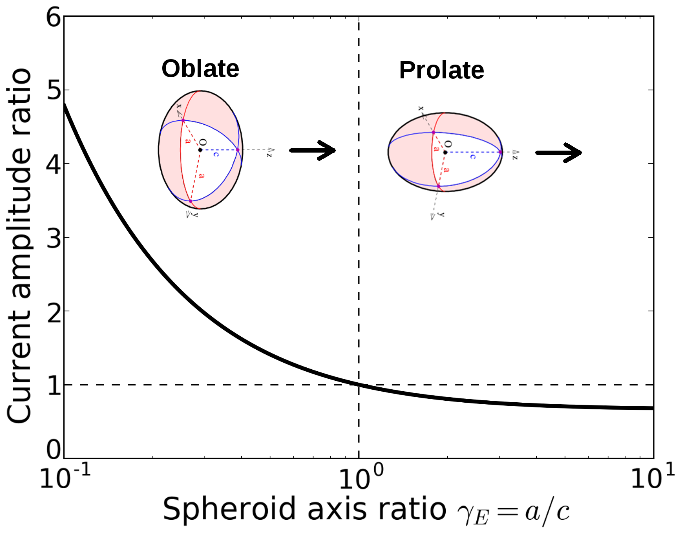
\includegraphics[width=0.5\textwidth]{dIellipsoid.png}
			\caption{\textbf{Resistive pulse amplitude $\Delta I/I_{p}$ for equal volume spheroidal objects relative to a sphere.} The polar axis of the particle is aligned with the channel's axis, so that oblate geometries correspond to motion along the channel axis. The values come from equation \ref{eq:ellipsoiddI} when the correct shape factor $f_{\parallel}$ is applied.}
		\end{figure}

		
		For spheres, $f_{\parallel}=1$, and for prolate and oblate spheroids, $f_{\parallel}<1$ and $f_{parallel}>1$, respectively. Figure \ref{fig:dIellipsoid} shows plots of the RP amplitude $\Delta I/I_{p}$ for ellipsoids of the same volume but different aspect ratios, relative to a sphere. The plot reveals that even for modest deformation, for instance a stretching ratio of $2/3$, a mildly oblate ellipsoid, the increase in $\Delta I/I$ is nearly $30\%$. Similarly, the current $\Delta I/I$ changes for prolate geometries, although to a lesser degree.
		
		As mentioned previously, there are many possible types of high throughput microfluidic systems than can induce cell deformations. We devised a method that has been shown to be capable of inducing bidirectional deformations (prolate and oblate). The key to understanding the channel geometry is to understand the primary hydrodynamic forces that work on a cell and deform it in extensional, i.e. accelerating and decelerating flows. When a cell transitions from a region of high local fluid velocity to low local fluid velocity, there is a greater magnitude of normal stress forces on the back of the particle than on the front. Consequently, the particle is pushed into a laterally elongated state, corresponding in our model to the oblate geometry. Oppositely, when the particle makes the transition from a slow to fast region, the net forces pulling the particle forward are greater than the forces pushing it from behind, elongating it in its direction of motion. This corresponds to the prolate shape configuration. According to this model, one can induce bidirectional shape changes in passing particles by having transitions between regions of slow and fast local fluid flow, and vice versa. This criterion allows for multiple possibilities, but the geometry chosen for our system is described by a channel having a central cavity, but otherwise with a straight cross-section. As the cell enters the microchannel, it accelerates and is pulled in, and in the process deforms into a prolate shape. When the cell arrives at the central cavity, the fluid flow is slower and the particle decelerates, becoming oblate. At the end of the cavity, the particle again undergoes an acceleration and deforms back into its prolate shape. Figure \ref{fig:channelscheme} shows an example image of one of the channel geometries used in this study, along with a scheme showing the deformation modes that occur in each region of the channel.
		
		Although the deformation dynamics are undoubtedly complicated, to first order we seek to find the aspect ratio of the approximate ellipses $a/b$ at various points in the channel. The aspect ratio will remain the same at all points for completely non-deforming particles, but will vary according to the above model for deforming particles, and to a greater degree for the most deformable particles. For the scheme shown in Fig. \ref{fig:channelscheme}, the expected aspect ratio $a/b$ as a function of the axial position adheres to the motif shown in Fig. \ref{fig:aspectmotif}. Besides size, the observables of interest might be the minimum and maximum aspect ratios, or perhaps the ratio of the minimum and maximum aspect ratios which would reflect the general elasticity properties of the cells. However, in the RP signal the actual deformation of the particles would be reflected in the changes in the measured $\Delta I/I_{p}$ signal \textit{relative to the expected $\Delta I/I_{p}$ of a completely non-deforming spherical particle of the same volume}. This means in the narrow regions where a prolate elongation occurs the current amplitude $\Delta I/I_{p}$ would be \textit{decreased}, while in the central cavity where the particle assumes an oblate geometry the signal would be \textit{increased}. Figure \ref{fig:RPmotif} shows an example RP event for a particle passing through the cavitated channels, and the distortion of the RP signal corresponding to the model described above. Therefore, the observable of interest might be the ratio of the maximum in the signal (minimum $\Delta I/I_{p}$) and either of the two minima in the signal (maximum $\Delta I/I_{p}$), which would be a proxy measurement for the ratios of the aspect ratios calculated directly from imaging data. For larger deformations, this ratio would increase as the signal distortion motif in Fig. \ref{fig:RPmotif} shows.
		
	\section{Experiment and data analysis}

		In order to test the concept of cell deformability cytometry with the channel geometry described above and using RP, we ran microfluidic experiments with cancer cells. Although the ultimate goal of this sensor will be to perform deformability cytometry with the RP signal alone, in order to test the method it is necessary to have a high-speed camera. In the following sections we describe the complete experimental set up, the software used to control the experimental instrumentation, and the data processing and analysis steps that take place after the experiment. To date, the experiments performed have primarily been focused on analyzing the optical data in the experiments, since measuring their deformability optically is a prerequisite for determining it via the RP signal.
	
		\subsection{Experiment and instrumentation control}
		
			The entities involved in the experiments include the microfluidic channels, the cells and the suspension media that holds them, a syringe pump to drive the suspension through the systems, a microscope and high-speed camera used to take the images, the data acquisition card (DAQ) that acquires the RP signal, a central control computer used to run the experiments,  and various other miscellaneous pieces of equipment. A more in-depth description of these components and the roles they play in the experiment is as follows.
			
			\begin{figure}
				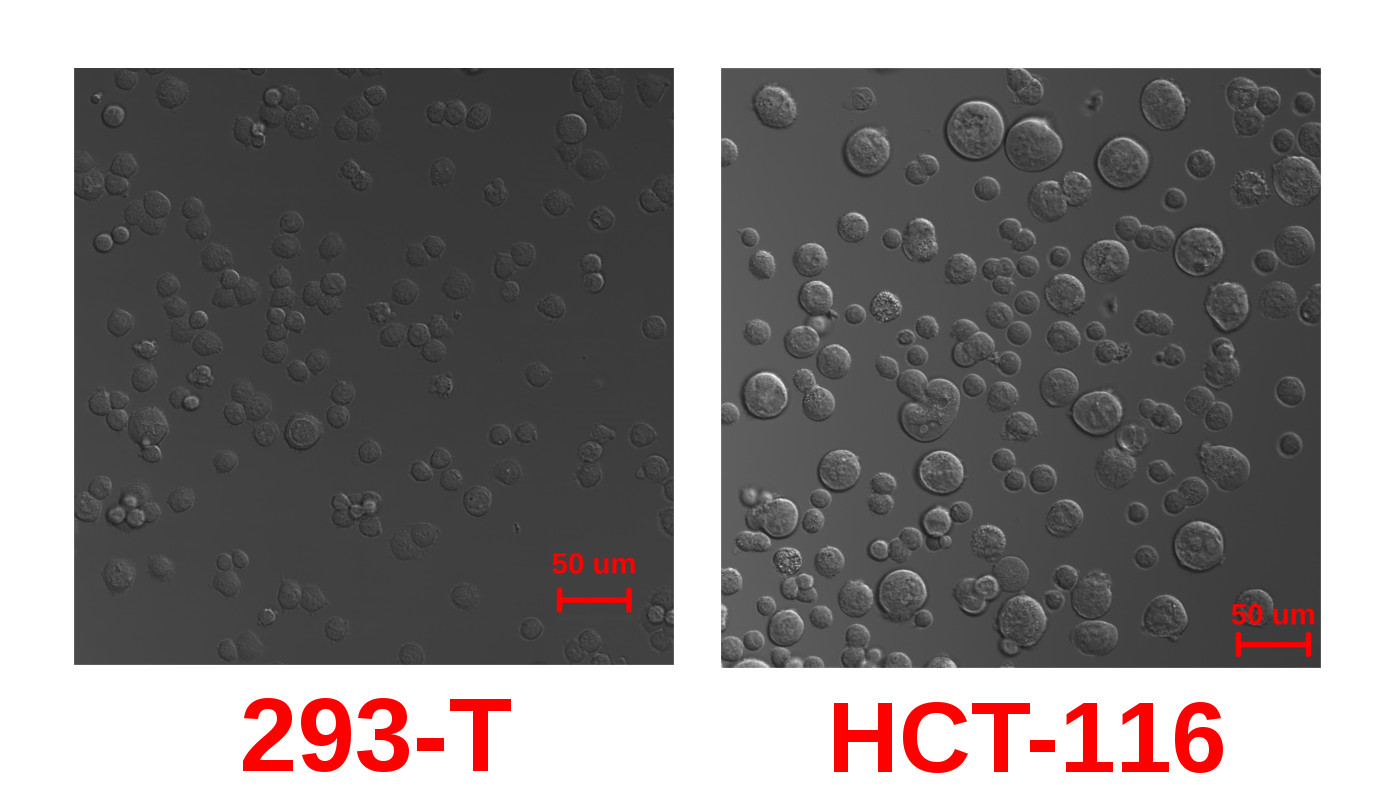
\includegraphics[width=\textwidth]{celllines.jpg}
				\caption{\textbf{Confocal images of 293-T (left) and HCT-116 (right) cells.} Scale bars are $\SI{50}{\mu m}$ long.}
				\label{fig:celllines}
			\end{figure}

			
			First, we start with the cells. Three human cell lines were provided for the experiments, chosen for the variety of deformation and size properties they exhibit. The cell lines are HCT-116 (colorectal cancer), 293-T (derived from human embryonic kidney cells), and THP-1 (monocytes). Images of the HCT-116 and 293-T cells are shown in Fig. \ref{fig:celllines}. The cells are filtered and diluted to a concentration of $0.5\times10^{6}/$mL or $1\times10^{6}/$mL in a solution of HBSS, a relatively highly conductive biocompatible buffer. In most experiments, the solution was doped with methylcellulose, another biocompatible component that increases the viscosity of the solution, which should promote cell deformations. Pluronic, a biocompatible surfactant, is added at $0.1\%$ concentration by volume.
			
			\begin{table}
				\begin{center}
				    \begin{tabular}{lrc}\hline
						Step name & Instrument & Parameters \\
						\hline
						Preprocess cleaning & Isoproponal & \\
						Wafer dehydrate & Dry oven & $95^{\circ}$C, $\SI{30}{min}$ \\
						First spin & Laurell spinner & (parameters) \\
						Second spin & Laurell spinner & F \\ \hline
						Soft bake (cold) & Hot plate & $65^{\circ}$C, $\SI{1}{min}$ \\
						Soft bake (hot) & Hot plate & $95^{\circ}$C, $\SI{5}{min}$ \\
						UV flood exposure & AMV & $\SI{52}{seconds}$ (intensity varies, adjust accordingly) \\
						Post-exposure bake (cold) & Hot plate & $65^{\circ}$C, $\SI{1}{min}$ \\
						Post-exposure bake (hot) & Hot plate & $95^{\circ}$C, $\SI{5}{min}$ \\
						SU8 develop & SU8 develop solution & $\SI{5}{min}$ soak, with periodic agitation of solution \\
						SU8 developer rinse & SU8 developer solution & \\Soft bake (hot) & Hot plate & $95^{\circ}$C, $\SI{5}{min}$ \\
						Post-photolithography bake & Hot plate & $95^{\circ}$C, $\SI{2}{hours}$ \\
						\hline
						PDMS preparation & Sylgard-184 and curing agent & 10:1 by volume Sylgard-184 to curing mix \\
						PDMS degassing & Vacuum & $\SI{30}{min}$ \\
						PDMS cure on SU8 mold & Hot plate & $75^{\circ}$C, $\SI{150}{min}$ \\
						PDMS-glass bond & Harrick-Plasma oxygen plasma chamber & $\SI{300}{mT}$, med. power, $\SI{35}{sec}$    
				    \end{tabular}
				    \caption{Class Mark List}\label{tab:devicefab}
				\end{center}
			\end{table}
			
			
			
			
			
			The microfluidic channels are fabricated \textit{via} standard, well-established soft photolithography techniques. Fabrication primarily takes place in a class 10000 clean room of the BiON facility at the University of California, Irvine. First, SU8-2025 photoresist is spun onto a $\SI{4}{inch}$ silicon wafer with the correct rotational speed to achieve a thickness of $\SI{20}{\mu m}$. A transparency with the channel design printed on with a high DPI printer is taped onto the SU8 side of the wafer, which is then exposed to a UV flood lamp. UV light passes through the non-printed parts of the transparency and reaches the SU8 photoresist. Polymer molecules in the exposed areas are cross-linked, resulting in these regions being more stable. The photomask is then removed, and the wafer soaked in SU8 developer solution until the non-crosslinked parts of the channel are completely washed away. The resulting structures left after the SU8 is washed away comprise the device mold. PDMS, a relatively chemically inert elastomer is degassed and then poured over the mold and baked until completely hardened. After curing, the PDMS layer is carefully pulled off the wafer, and individual microfluidic devices are cut out. The inlet and outlet access ports are punched through with a biopsy punch. Finally, the PDMS device and glass slide are treated in an oxygen plasma which temporarily alters the chemical composition of the surfaces, allowing for bonding. After being taken out of the plasma, the glass slide and PDMS layer are quickly but delicately pressed together, resulting in a quick bonding. Table \ref{tab:devicefab} contains a list of the key steps involved in the device fabrication, the particular instrument(s) used in each step, and all main parameters relevant to those instruments operations in this application.
			
			Once the device is fabricated, it is taped onto the glass stage of the optical microscope. The high-speed camera is mounted on to the microscope, where the light is directed instead of into the eyepiece. Plastic tubing, which serves as the fluid access, is inserted into the inlet and outlet ports. Ag-AgCl electrodes are inserted into the tubing as well, as close as possible to the actual microfluidic device. The electronic set up used to make RP measurements consists of a patch clamp amplifier, which in its current configuration merely applies a voltage, and a lower amplification amplifier. This circuit is connected to a BNC breakout box, which connects to the data acquisition card via a parallel data bus, which actually streams the measured RP data. A syringe containing the particle solution is inserted into the inlet tubing with a luer lock configuration, and the syringe is mounted onto a syringe pump which is used to drive the solution through the channel. Finally, the syringe, high-speed camera, and data acquisition card are all connected into a central control computer which is used to command the three instruments and save their data locally. Figure \ref{fig:hardwarescheme} shows a scheme of the hardware implementation used for the experiment.
			
			In order to control the three insruments and save data, a graphical user interface (GUI) program was written. The program was written in C++ and the Qt Framework, and uses threading to ensure asynchronous operation of the three instruments, as well as the controls in the GUI itself. Communication protocols used were specific to each of the hardware instruments. The software communicates with the syringe pump \textit{via} a serial RS-232 communications protocol. Communication with the high-speed camera occurs over TCP/IP protocol over a 1 Gb ethernet line, with instructions specific to the camera's manufacturer. Lastly, the DAQ card is controlled via the niDAQMX software library. The software allows the user to perform all operations on the syringe pump remotely. When not recording, the software displays live images from the camera feed that show the view through the microscope. The user may also change the camera's recording parameters such as frames per second, exposure rate, and pixel resolution, and when ready, to record videos and save the data to the computer after recording. Similarly, the software also displays the RP data stream and can save it as well. Figure \ref{fig:cellcontroller} shows an image of the GUI program; the software is open-sourced and available at https://github.com/tphinkle/cell\_controller.
			
			After the cell suspension is prepared and the experiment set up, data recording occurs. The syringe pump is started so that the solution is driven through the microfluidic channels. The initial `push' of the syringe pump is usually much greater than needed, which serves two purposes. First, it quickly pushes the solution from the syringe pump to the actual device. Sedimentation due to gravity is significant for the cells used here, so a quick start to the experiments is highly desirable in order to ensure high event frequency during recording. The second purpose of pushing solution very rapidly is that it puts the fluid into a turbulent regime. In this regime, the regions of solution adjacent to the exit of the channel display stable turbulent vortical flows, and are very likely to capture cells. These trapped cells provide a target by which to focus the microscope; due to the extremely small size of the channels, even under small latent pressures in the system (i.e., without pushing on the syringe pump), cells move far too quickly to properly focus on, usually staying in the field of view of the camera for only a single frame in the GUI's view. However, while the cells trapped in the vortical flows at the channel's exit are rapidly moving, they do not leave the field of view of the camera and therefore act as a moving target on which to focus the microscope. This unconventional trick has proven absolutely invaluable in the experimental workflow, as the focus required to obtain good camera images of the cells is very sensitive. In unfocused images, while cells may be detected their boundaries are often non-resolvable. After the proper focus has been established, the flow rate is reduced to the desired flow rate that the user wishes to record, and a fixed amount of time is waited to allow the fluid to equilibrate. After this delay, both the RP and camera signal are recorded. While the recording itself is very fast, the data must be transferred to the control computer in order for it to be stored; the onboard camera memory is only sufficient to hold the data of a single recording. The transfer and saving process takes nearly 15 minutes, and over this duration of time the vast majority of cells sediment to the bottom of the tubing and syringe. For this reason, in between data transfers we remove the tubing and syringe and clean them. After recording, the solution is gently mixed to resuspend the cells, and the process of pushing the solution, refocusing the microscope, and recording is repeated. Experiments are repeated in this way for different cell lines, channel geometries, and fluid flow rates. Following the experiments, data is immediatley backed up redundantly to external storage drives where it remains until it is ready for post processing and analysis.
		
		
		
		\subsection{Data analysis}
			
			The data generated from these experiments includes the imaging data from the camera and the resistive pulse data. In order to analyze this unique combination of data sets, a library called pore\_stats was written in Python. pore\_stats was primarily written for the purpose of analyzing resistive pulse data, however image processing functions were added to analyze the data from these hybrid RP-IM experiments. Pore\_stats is discussed in greater detail in chapter \ref{chap:rpim}
			
			The primary observable of interest in this experiment is the shape of the particle. There is no single way of defining the shape of an object, but because we are interested in comparing the RP signals of cells with the theoretical RP amplitudes of ellipses, we determine the shape of the cell by fitting ellipses to its borders across multiple frames. Thus, the objective in demonstrating deformation optically is to fit ellipses with semi-major axis $a$ and semi-minor axis $b$ to cells across multiple frames and track their change in aspect ratio as they pass through the channel. According to the above model, the cells should oscillate between prolate, oblate, and spherical shapes at various points in the channel, and therefore we expect to observe an oscillation of the determined aspect ratio $\gamma=a/b$ between values $>1$ and values $<1$. The exact shape of the cell is never exactly ellipsoidal, however we find that for most shape configurations it is an adequate approximation.
			
			
			\begin{figure}
				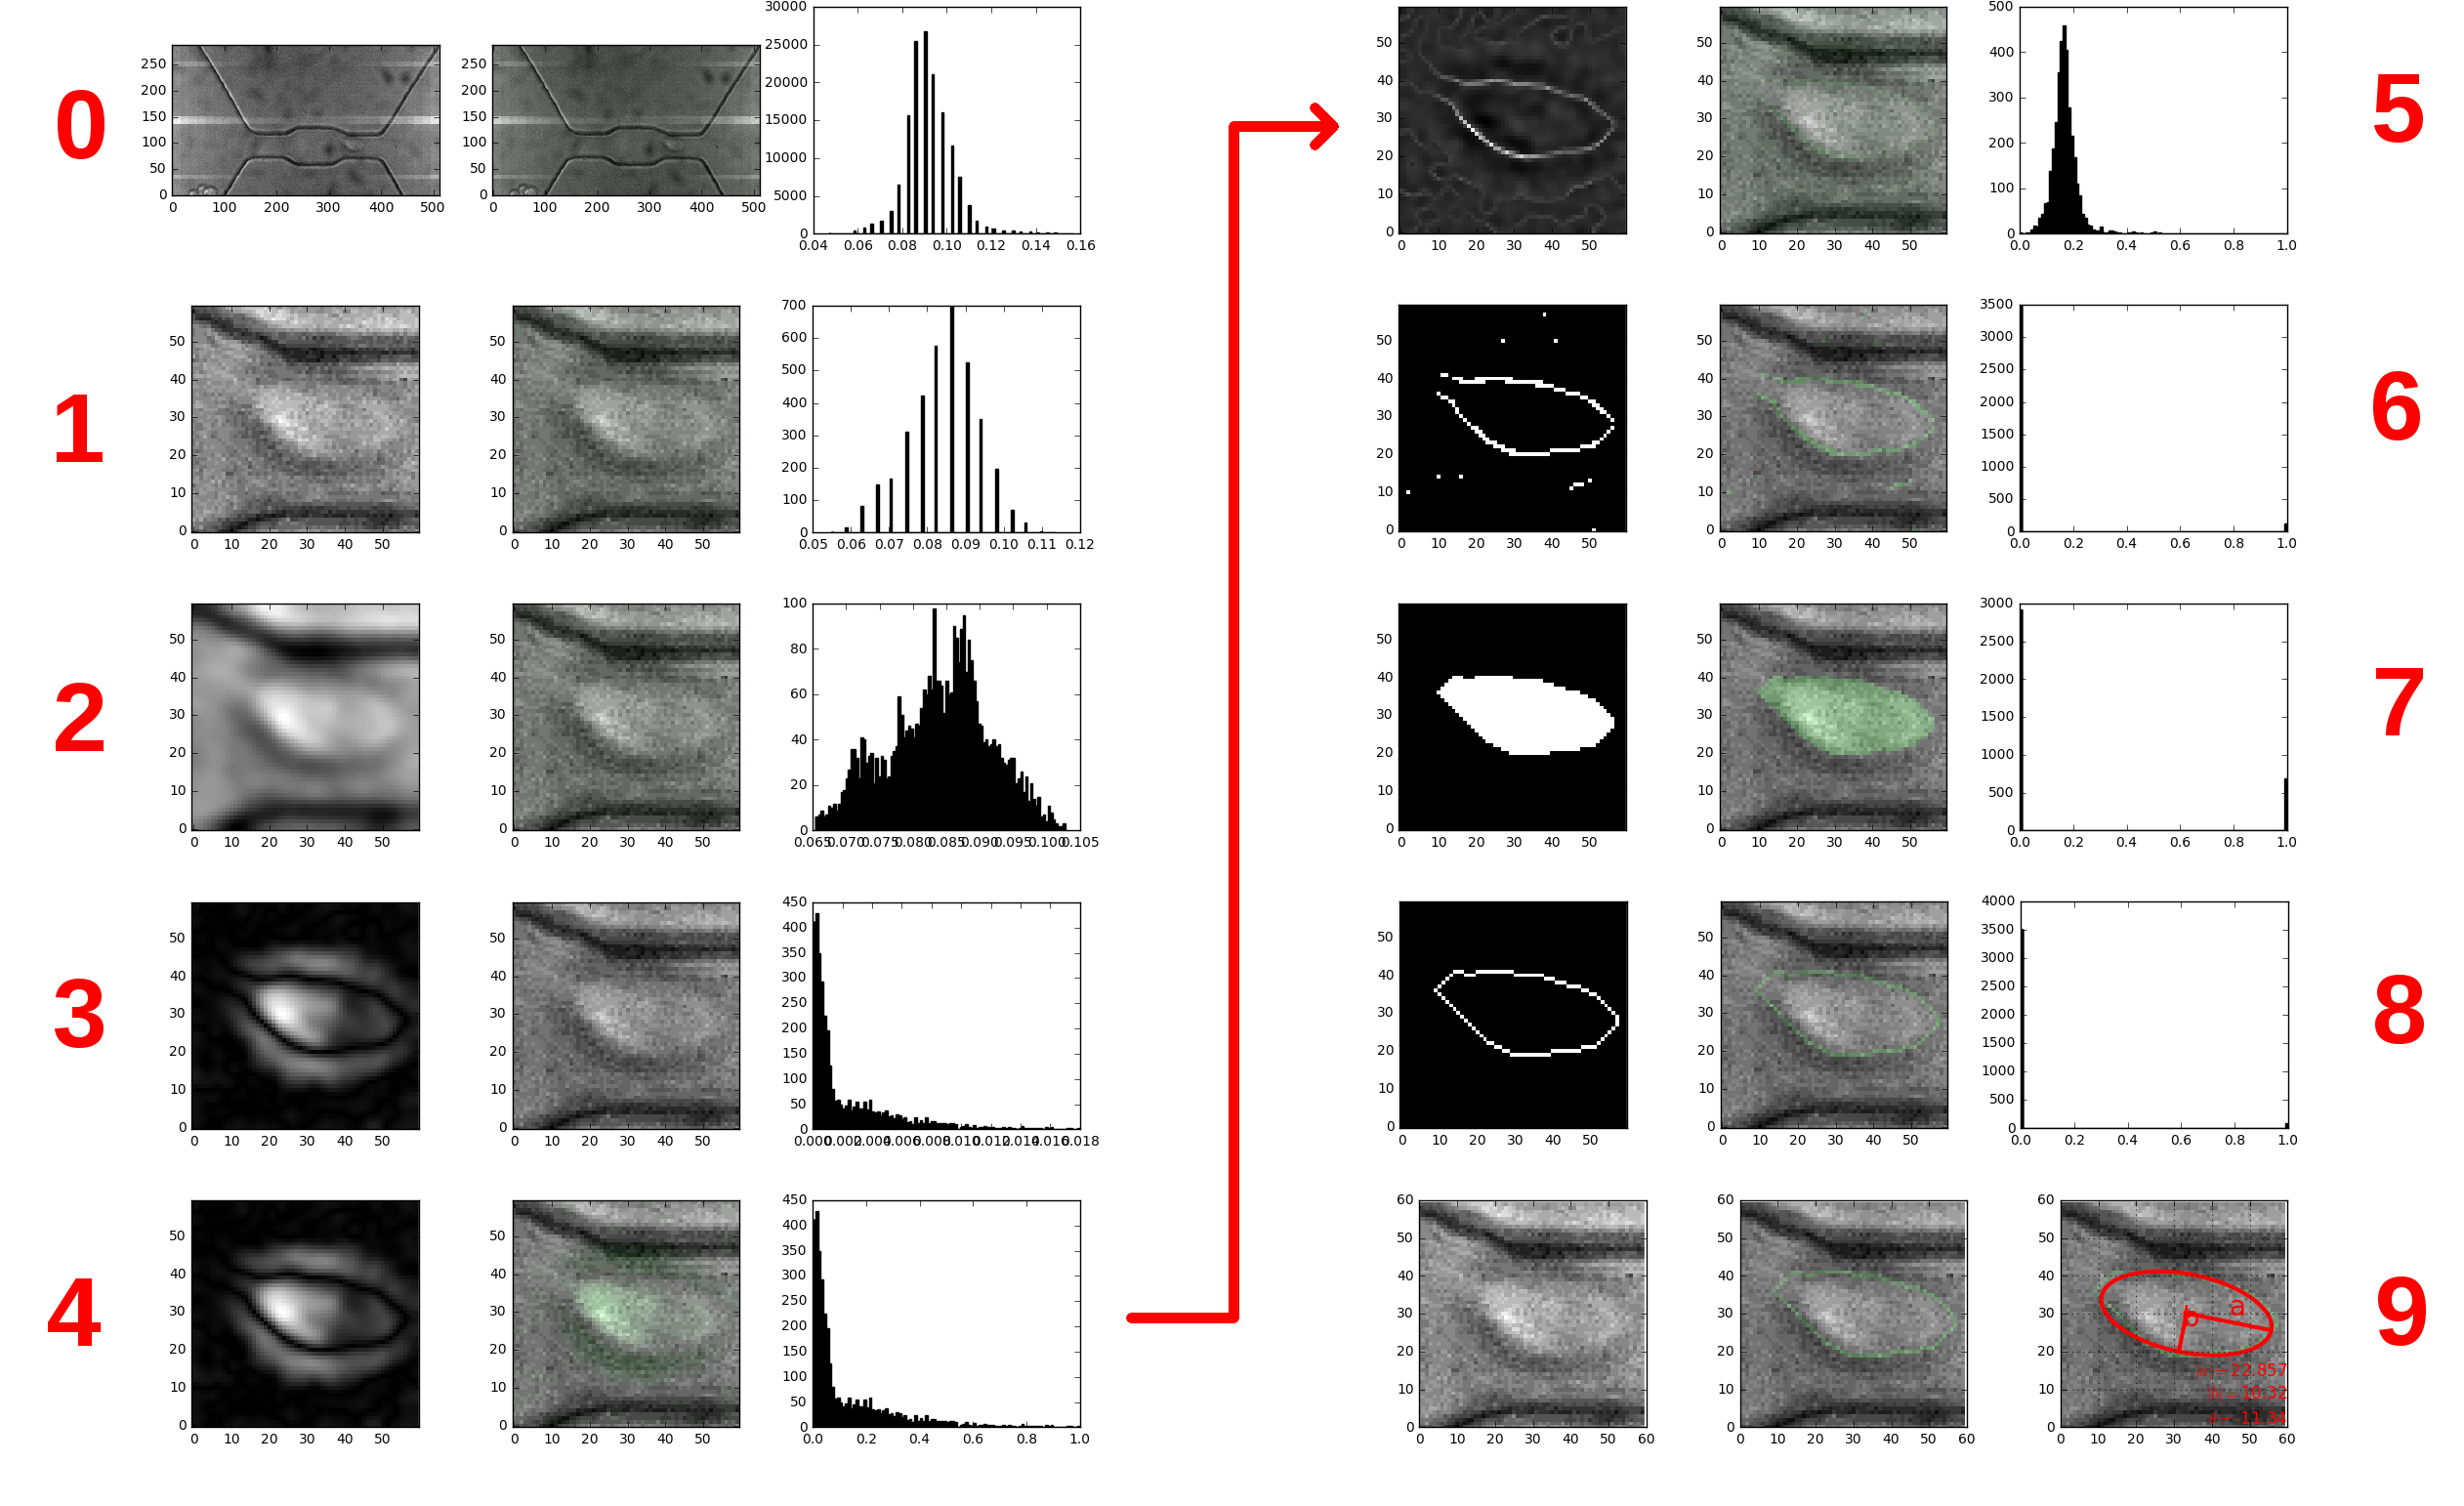
\includegraphics[width=\textwidth]{ellipsefittingprotocol.png}
				\caption{\textbf{Example ellipse fitting protocol for a single detection within a single event.} The left column of each row shows the current image transformation. The central column shows the raw frame with the pixels shaded green with intensity according to the intensity of the pixels in the transformed image. The right column shows pixel intensity in the processed image. \textbf{1: } Raw image. \textbf{2:} Image is cropped in the vicinity of the particle. \textbf{3:} Template image is subtracted off. \textbf{4:} Pixel intensity is rescaled. \textbf{5:} Laplacian derivative. \textbf{6:} Pixel intensity thresholding. Notice the histogram becomes binary distributed. \textbf{7:} Morphological closing of image. \textbf{8:} Image is dilated and subtracted from undilated image, leaving a thin shell around the border of the cell. \textbf{9:} Ellipse is fit to the cell's border.}
				\label{fig:ellipsefittingprotocol}
			\end{figure}

			
			
			While the ellipses could be fit manually by determining the width and height of the channel in each frame, the number of cells observed prohibits this manual measurement. Instead, we devise an image processing pipeline that starts with the raw camera data and results in a calculation of the ellipse fits for every single detection and every single particle passing through the channel. The pipeline works as follows. First, cells are detected in individual frames via a template subtraction method. Then, cells are tracked across frames using a minimum distance approach. These two methods are described in greater detail in chapter \ref{chap:rpim}. After a list of events is determined, ellipses need to be fit to the image of the cell in each frame. A number of preprocessing steps is required to transform the image to a form where this ellipse fitting is possible. One possible ellipse fitting protocol is shown in Fig. \ref{fig:ellipsefittingprotocol}. All processing protocols must reduce the image down to a binary form where the only pixels highlighted are the pixels on the exact boundary of the cell. Operations common to most processing protocols are template subtraction, Gaussian blurring, Laplace derivative transformation, thresholding, and morphological operations such as binary dilation, erosion, and closing. The end result is shown in Fig. \ref{fig:ellipsefittingprotocol}, row 9. Fitting an ellipse to the particle in each frame is useful because many properties of the particle and its translocation can be determined via the ellipse fits. For instance, ellipse fitting yields accurate determination of the central position of the particle, which can be used to accurately determine its trajectory and velocity. Furthermore, once the ellipse is obtained for every frame it is easy to calculate the aspect ratio of the particle during the course of its trajectory and compare with the expectations of the model proposed earlier (Fig. \ref{fig:deformationmotif}.
			
			
	
	\section{Results \& Discussion}
	
		\begin{figure}
			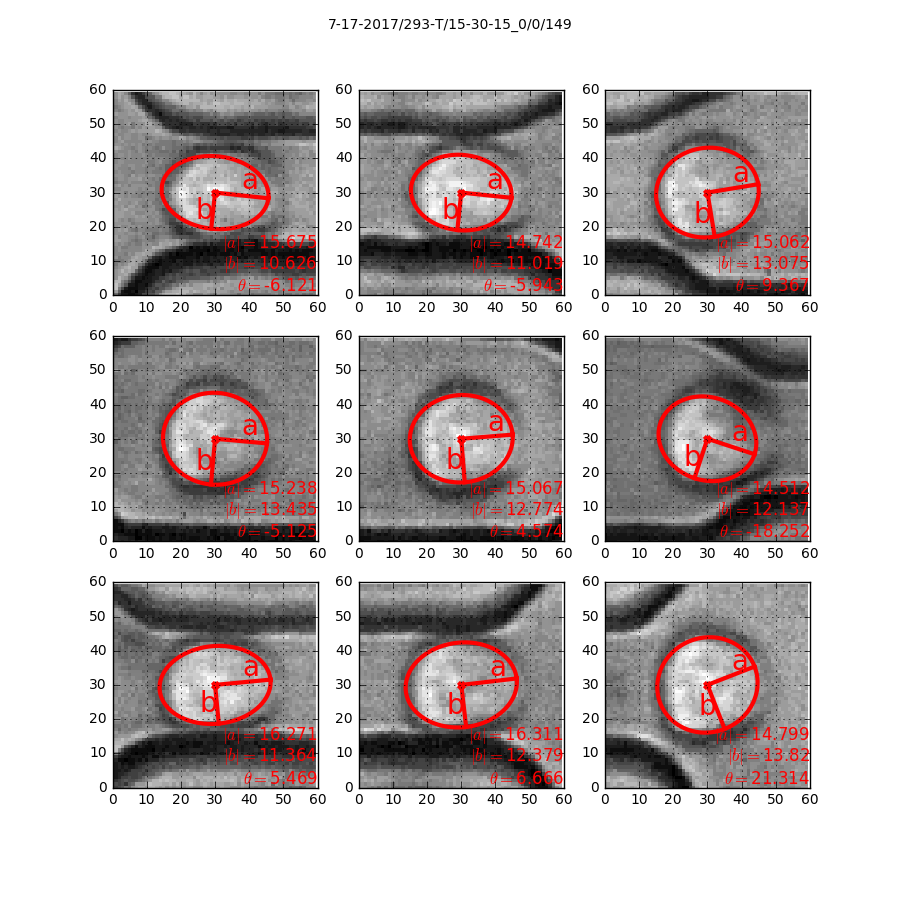
\includegraphics[width=0.5\textwidth]{ellipses.png}
			\caption{\textbf{Ellipse fits for a 293-T cell passing through a $15-30-15 \mu\mathrm{m}$ channel at various positions.} Notice that in the narrow portions of the channel the particle assumes a prolate (axially-elongated) shape, while in the central cavity it assumes an oblate (laterally-elongated) shape, in agreement with the motif presented in Fig. \ref{fig:deformationmotif}}.
			\label{fig:ellipses}
		\end{figure}

	
		The most important question to be answered in the experiments is whether the cells actually deform according to the model proposed. In order to answer this question, we examined specific events to look at their change in aspect ratio as they pass through the channel. Many events consistently show a deformation pattern that subscribes to the model, as shown in Fig. \ref{fig:ellipses}. On the other hand, there were many events that showed modest to little deformation. However, this result is not unreasonable; our model does not suggest that all cells must deform, and indeed there may be cells that are quite resilient to deformations, or cases where the hydrodynamic forces were insufficient to generate significant deformation. However, we never observe a trend opposite to the deformation mode posited, i.e. an oblate-to-prolate transition rather than a prolate-to-oblate transition. This observation suggests that, while the magnitude of the effect may be low in some cases, the effect still occurs.

		

		
		


%%% Local Variables: ***
%%% mode: latex ***
%%% TeX-master: "thesis.tex" ***
%%% End: ***

\graphicspath{{../images/ch5/}}	% Image directory


\chapter{Resistive pulse studies of cancer cell deformability}
\label{chap:cell}

	

	\section{Background \& Theory}
	      
		One of the most important applications in microfluidic technology today is the study of cell populations. The most important tool for studying cell properties is the flow cytometer, invented in 1965 by Fulwyler \cite{Fulwyler1965}, and is conceptually the follow up to Coulter counters which can be considered to be impedance cytometers. Flow cytometers are a mixture of many individual microfluidic elements combined in series, each with its own function. On the sensing side, flow cytometry makes use of measured scattering of laser light as well as detection of fluorescence signals. Dyes are specifically attached to certain types of antibodies, which then may interact with the cell membranes in the suspension. When the cells are pulsed by lasers in the laser light, it stimulates emission of specific dyes, which can be measured to determine which antibodies have interacted with the cell. This type of information is incredibly value in determining phenotypic and classification information for the cells. Furthermore, the information garnered from real-time cytometry information can be used to sort cells in real time, in a system known as fluorescence activated cell sorting system (FACS). Cell cytometry is the workhorse of modern day molecular and cellular biology studies, but suffers from the fact that it is a label-dependent method due to the introduction of the dyes. Such labels can adversely affect the the cells' viability that prevents them from being used in a post-interrogation analysis, even after being separated by a system like FACS. Additionally, flow cytometry requires the use of costly fluorescent reagents and skilled technicians that must be present to perform the measurement and to ensure proper calibration of the fluorescence signal \textit{via} the use of fluorescent beads \cite{Gosset2012} (DiCarlo PNAS).
	
		While flow cytometry focuses on the measurement of cells' interactions with specific antibodies, another dimension often not thought of is the cells' mechanical properties, such as their size, shape, deformability, and deformability dynamics \cite{Lin2017} (DiCarlo paper in Nature 2017). Since their discovery, we've known that a wide variety of cell sizes exist, but more recently scientists have focused on the difference in the mechanical stiffness of cells. Cell stiffness has been shown to vary from cell to cell, and even between various stages in cells' mitotic cycles. As a concrete example, cancer cells are known to be generally `squishier' than non-cancerous cells. For these reasons, developing a method of probing the mechanical stiffness of cells is highly desirable for cell characterization applications, and serve as a complementary cell phenotyping platform to deformability cytometry.
		
		In order to measure the stiffness of an object, it must be subjected to constrained forces and its response measured. Probably the most straight forward way of doing this is by directly applying a mechanical force on the cell, for example by using an atomic force microscopy (AFM) probe to directly press on the cells and measure the resultant recoil force felt by the AFM's cantilever, which is directly related to the Young's modulus of the cell. Other similar methods exist, and while they are very accurate and easily interpretable, they suffer from an excruciatingly slow throughput. For instance, using AFM for cell deformation measurement can take a few minutes per cell. For cell applications a high throughput is necessary, and therefore these applications are not feasible for discovering cell population statistics.
		
		Another method of measuring cell deformability is with microfluidics platforms. Cells passing quickly through narrow constrictions are subjected to large, anisotropic hydrodynamic forces, and these forces can induce a measurable particle deformation. The advantage of this type of method is its extremely large throughput; rather than spending several minutes per particle as in measurements conducted with AFM, thousands of cells per second can be measured in microfluidic platforms. Even within the narrow field of microfluidic-based deformability cytometry, there are multiple types of platforms. Probably the most conceptually simple is a standard microfluidic channel that tightly confines cells passing through it. Due to anisotropies in the hydrodynamic stresses and strains around the particle, it will deform even in a uniformly shaped channel.
		
		In traditional microfluidic methods of measuring cell deformability, direct imaging is used to determine the cell shape across different frames in the video, which corresponds to the hydrodynamic load it is under. However, for the high throughputs that are the reason why people use microfluidics, camera imaging must be performed very quickly. This requires the use of a high-speed camera used in conjunction with an optical microscope, usually shooting at a minimum of $\SI{10000}{fps}$. When combined with an optical microscope, such high-speed cameras are capable of capturing cell deformations with high spatial and temporal resolution, and are even capable of resolving the cells' deformation dynamics \cite{DiCarlo2017}. Currently high-speed camera imaging is by far the most popular method of capturing cell deformations, but it comes with two serious disadvantages. First, the camera itself adds a large cost to the apparatus, and will likely dwarf the price of any other component in the deformability cytometer. Second, imaging data is inherently highly multidimensional and computationally expensive to analyze. As a result, online analyses conducted during the run of the experiment are usually not possible at the flow rates that these experiments operate at. While the data can still be stored, processed, and analyzed later, offline analysis does not allow for real-time separation, one of the most highly desirable applications of this type of metrology.
		
		Instead of using camera imaging, one can instead imagine trying to employ resistive pulse (RP) to measure the deformability of particles. In terms of practicality, RP is far more computationally light than imaging data, as the following order of magnitude estimate shows. First, consider the data bandwidth in high-speed imaging. Passage through a deformability cytometry system may consist of $\sim100$ frames, each with a resolution of perhaps $100x50$ 8-bit grayscale valued pixels. As a result, a single translocation is described by $\SI{500}{kB}$ worth of data. At a rate of $1000$ particles per second, this corresponds to a raw data throughput of $\SI{500}{MB/s}$ of data that must be processed. Finally, in a common image processing algorithm the number of computations performed on each pixel is probably greater than one; identifying the shape of an object in a frame certaintly consists of multiple serial image processing steps. Although this is just an estimate, it conveys the point that high-speed imaging is not amenable to online analysis, especially at the throughputs that are desired for these types of calculations. On the other hand, consider a resistive pulse analysis: under the same criteria described above, an RP data stream being sampled at $\SI{1}{MHz}$ will consist of a data throughput of only $\SI{1}{MB/s}$, a factor of $500$ decrease in raw data throughput. Furthermore, the types of operations needed to extract deformability information from the raw RP signal are also computationally light relative to image processing techniques.
		
		While it is apparent that resistive pulse is computationally cheaper than imaging analysis, it is most important to demonstrate that deformability can actually be measured via RP sensing. In chapter 4 of this dissertation, we discussed the equations for the resistive pulse amplitudes of ellipsoidal objects. For cells that are spheroidal in their unloaded state, ellipsoids are reasonable geometries to expect for the deformation shape in the loaded state, at least as an approximation. If we consider a straight ion conducting channel with an ellipsoidal particle inside it, the aspect ratio and orientation of the particle greatly affects the ionic resistance of the system. Under the assumption that the particles take on ellipsoidal geometries, the shapes will be described as being prolate, oblate, or spherical with respect to the channel's axis. Oblate geometries correspond to a flattening along the channel's axis, and prolate geometries are an extension along the channel's axis. The difference in the measured resistive pulse amplitude of these particles is given by the following equation:
		
		\begin{equation}\label{eq:ellipsoiddI}
			\frac{\Delta I}{I_{p}}=f_{\parallel}\frac{v}{V},
		\end{equation}
		
		where $v$ and $V$ are the volume of the particle and channel, respectively, and $f_{\parallel}$ is a constant known as the `shape-factor', which depends on the aspect ratio of the ellipsoid. 
		
		\begin{figure}
			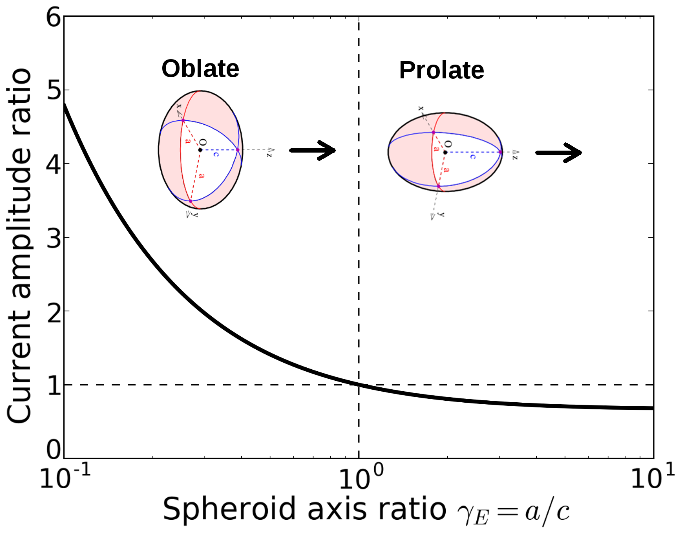
\includegraphics[width=0.5\textwidth]{dIellipsoid.png}
			\caption{\textbf{Resistive pulse amplitude $\Delta I/I_{p}$ for equal volume spheroidal objects relative to a sphere.} The polar axis of the particle is aligned with the channel's axis, so that oblate geometries correspond to motion along the channel axis. The values come from equation \ref{eq:ellipsoiddI} when the correct shape factor $f_{\parallel}$ is applied.}
		\end{figure}

		
		For spheres, $f_{\parallel}=1$, and for prolate and oblate spheroids, $f_{\parallel}<1$ and $f_{parallel}>1$, respectively. Figure \ref{fig:dIellipsoid} shows plots of the RP amplitude $\Delta I/I_{p}$ for ellipsoids of the same volume but different aspect ratios, relative to a sphere. The plot reveals that even for modest deformation, for instance a stretching ratio of $2/3$, a mildly oblate ellipsoid, the increase in $\Delta I/I$ is nearly $30\%$. Similarly, the current $\Delta I/I$ changes for prolate geometries, although to a lesser degree.
		
		As mentioned previously, there are many possible types of high throughput microfluidic systems than can induce cell deformations. We devised a method that has been shown to be capable of inducing bidirectional deformations (prolate and oblate). The key to understanding the channel geometry is to understand the primary hydrodynamic forces that work on a cell and deform it in extensional, i.e. accelerating and decelerating flows. When a cell transitions from a region of high local fluid velocity to low local fluid velocity, there is a greater magnitude of normal stress forces on the back of the particle than on the front. Consequently, the particle is pushed into a laterally elongated state, corresponding in our model to the oblate geometry. Oppositely, when the particle makes the transition from a slow to fast region, the net forces pulling the particle forward are greater than the forces pushing it from behind, elongating it in its direction of motion. This corresponds to the prolate shape configuration. According to this model, one can induce bidirectional shape changes in passing particles by having transitions between regions of slow and fast local fluid flow, and vice versa. This criterion allows for multiple possibilities, but the geometry chosen for our system is described by a channel having a central cavity, but otherwise with a straight cross-section. As the cell enters the microchannel, it accelerates and is pulled in, and in the process deforms into a prolate shape. When the cell arrives at the central cavity, the fluid flow is slower and the particle decelerates, becoming oblate. At the end of the cavity, the particle again undergoes an acceleration and deforms back into its prolate shape. Figure \ref{fig:channelscheme} shows an example image of one of the channel geometries used in this study, along with a scheme showing the deformation modes that occur in each region of the channel.
		
		Although the deformation dynamics are undoubtedly complicated, to first order we seek to find the aspect ratio of the approximate ellipses $a/b$ at various points in the channel. The aspect ratio will remain the same at all points for completely non-deforming particles, but will vary according to the above model for deforming particles, and to a greater degree for the most deformable particles. For the scheme shown in Fig. \ref{fig:channelscheme}, the expected aspect ratio $a/b$ as a function of the axial position adheres to the motif shown in Fig. \ref{fig:aspectmotif}. Besides size, the observables of interest might be the minimum and maximum aspect ratios, or perhaps the ratio of the minimum and maximum aspect ratios which would reflect the general elasticity properties of the cells. However, in the RP signal the actual deformation of the particles would be reflected in the changes in the measured $\Delta I/I_{p}$ signal \textit{relative to the expected $\Delta I/I_{p}$ of a completely non-deforming spherical particle of the same volume}. This means in the narrow regions where a prolate elongation occurs the current amplitude $\Delta I/I_{p}$ would be \textit{decreased}, while in the central cavity where the particle assumes an oblate geometry the signal would be \textit{increased}. Figure \ref{fig:RPmotif} shows an example RP event for a particle passing through the cavitated channels, and the distortion of the RP signal corresponding to the model described above. Therefore, the observable of interest might be the ratio of the maximum in the signal (minimum $\Delta I/I_{p}$) and either of the two minima in the signal (maximum $\Delta I/I_{p}$), which would be a proxy measurement for the ratios of the aspect ratios calculated directly from imaging data. For larger deformations, this ratio would increase as the signal distortion motif in Fig. \ref{fig:RPmotif} shows.
		
	\section{Experiment and data analysis}

		In order to test the concept of cell deformability cytometry with the channel geometry described above and using RP, we ran microfluidic experiments with cancer cells. Although the ultimate goal of this sensor will be to perform deformability cytometry with the RP signal alone, in order to test the method it is necessary to have a high-speed camera. In the following sections we describe the complete experimental set up, the software used to control the experimental instrumentation, and the data processing and analysis steps that take place after the experiment. To date, the experiments performed have primarily been focused on analyzing the optical data in the experiments, since measuring their deformability optically is a prerequisite for determining it via the RP signal.
	
		\subsection{Experiment and instrumentation control}
		
			The entities involved in the experiments include the microfluidic channels, the cells and the suspension media that holds them, a syringe pump to drive the suspension through the systems, a microscope and high-speed camera used to take the images, the data acquisition card (DAQ) that acquires the RP signal, a central control computer used to run the experiments,  and various other miscellaneous pieces of equipment. A more in-depth description of these components and the roles they play in the experiment is as follows.
			
			\begin{figure}
				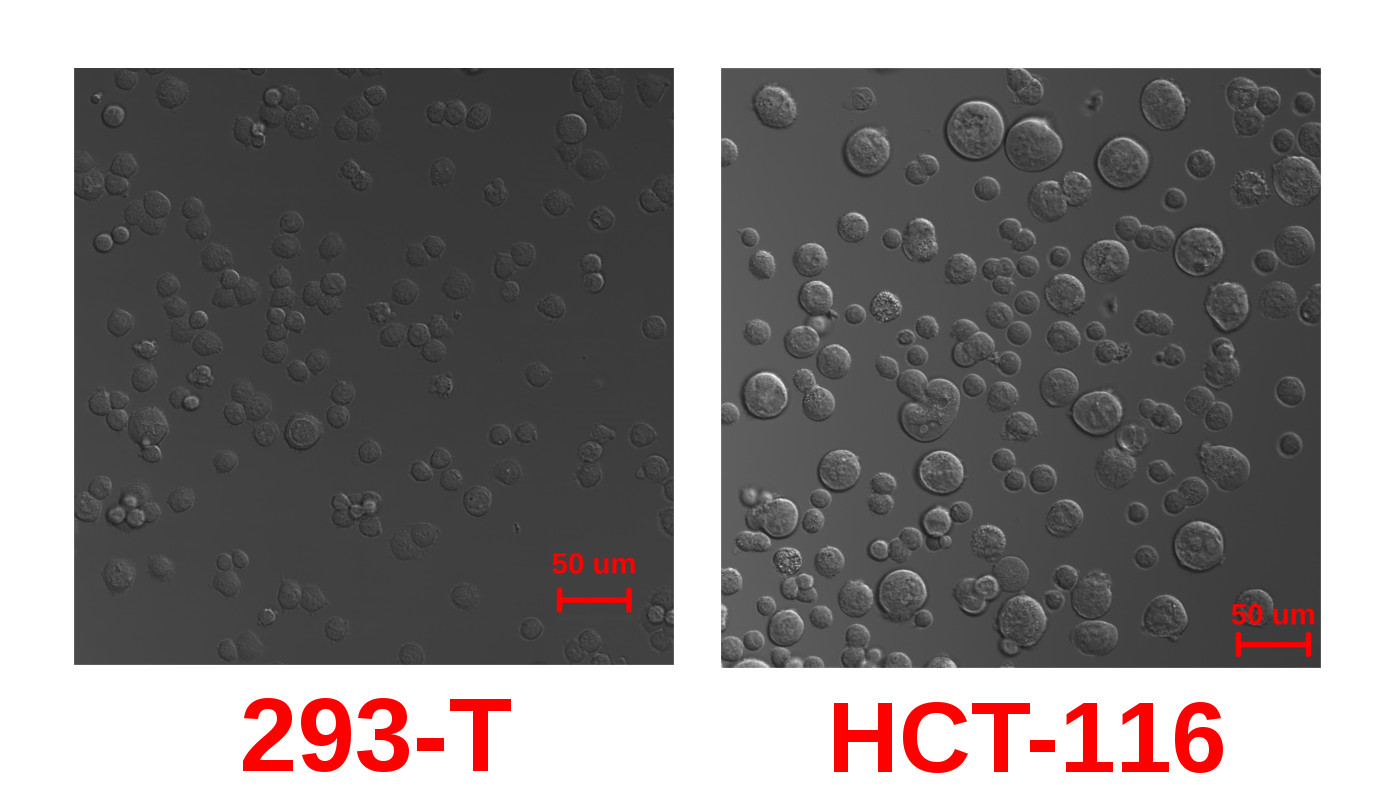
\includegraphics[width=\textwidth]{celllines.jpg}
				\caption{\textbf{Confocal images of 293-T (left) and HCT-116 (right) cells.} Scale bars are $\SI{50}{\mu m}$ long.}
				\label{fig:celllines}
			\end{figure}

			
			First, we start with the cells. Three human cell lines were provided for the experiments, chosen for the variety of deformation and size properties they exhibit. The cell lines are HCT-116 (colorectal cancer), 293-T (derived from human embryonic kidney cells), and THP-1 (monocytes). Images of the HCT-116 and 293-T cells are shown in Fig. \ref{fig:celllines}. The cells are filtered and diluted to a concentration of $0.5\times10^{6}/$mL or $1\times10^{6}/$mL in a solution of HBSS, a relatively highly conductive biocompatible buffer. In most experiments, the solution was doped with methylcellulose, another biocompatible component that increases the viscosity of the solution, which should promote cell deformations. Pluronic, a biocompatible surfactant, is added at $0.1\%$ concentration by volume.
			
			\begin{table}
				\begin{center}
				    \begin{tabular}{lrc}\hline
						Step name & Instrument & Parameters \\
						\hline
						Preprocess cleaning & Isoproponal & \\
						Wafer dehydrate & Dry oven & $95^{\circ}$C, $\SI{30}{min}$ \\
						First spin & Laurell spinner & (parameters) \\
						Second spin & Laurell spinner & F \\ \hline
						Soft bake (cold) & Hot plate & $65^{\circ}$C, $\SI{1}{min}$ \\
						Soft bake (hot) & Hot plate & $95^{\circ}$C, $\SI{5}{min}$ \\
						UV flood exposure & AMV & $\SI{52}{seconds}$ (intensity varies, adjust accordingly) \\
						Post-exposure bake (cold) & Hot plate & $65^{\circ}$C, $\SI{1}{min}$ \\
						Post-exposure bake (hot) & Hot plate & $95^{\circ}$C, $\SI{5}{min}$ \\
						SU8 develop & SU8 develop solution & $\SI{5}{min}$ soak, with periodic agitation of solution \\
						SU8 developer rinse & SU8 developer solution & \\Soft bake (hot) & Hot plate & $95^{\circ}$C, $\SI{5}{min}$ \\
						Post-photolithography bake & Hot plate & $95^{\circ}$C, $\SI{2}{hours}$ \\
						\hline
						PDMS preparation & Sylgard-184 and curing agent & 10:1 by volume Sylgard-184 to curing mix \\
						PDMS degassing & Vacuum & $\SI{30}{min}$ \\
						PDMS cure on SU8 mold & Hot plate & $75^{\circ}$C, $\SI{150}{min}$ \\
						PDMS-glass bond & Harrick-Plasma oxygen plasma chamber & $\SI{300}{mT}$, med. power, $\SI{35}{sec}$    
				    \end{tabular}
				    \caption{Class Mark List}\label{tab:devicefab}
				\end{center}
			\end{table}
			
			
			
			
			
			The microfluidic channels are fabricated \textit{via} standard, well-established soft photolithography techniques. Fabrication primarily takes place in a class 10000 clean room of the BiON facility at the University of California, Irvine. First, SU8-2025 photoresist is spun onto a $\SI{4}{inch}$ silicon wafer with the correct rotational speed to achieve a thickness of $\SI{20}{\mu m}$. A transparency with the channel design printed on with a high DPI printer is taped onto the SU8 side of the wafer, which is then exposed to a UV flood lamp. UV light passes through the non-printed parts of the transparency and reaches the SU8 photoresist. Polymer molecules in the exposed areas are cross-linked, resulting in these regions being more stable. The photomask is then removed, and the wafer soaked in SU8 developer solution until the non-crosslinked parts of the channel are completely washed away. The resulting structures left after the SU8 is washed away comprise the device mold. PDMS, a relatively chemically inert elastomer is degassed and then poured over the mold and baked until completely hardened. After curing, the PDMS layer is carefully pulled off the wafer, and individual microfluidic devices are cut out. The inlet and outlet access ports are punched through with a biopsy punch. Finally, the PDMS device and glass slide are treated in an oxygen plasma which temporarily alters the chemical composition of the surfaces, allowing for bonding. After being taken out of the plasma, the glass slide and PDMS layer are quickly but delicately pressed together, resulting in a quick bonding. Table \ref{tab:devicefab} contains a list of the key steps involved in the device fabrication, the particular instrument(s) used in each step, and all main parameters relevant to those instruments operations in this application.
			
			Once the device is fabricated, it is taped onto the glass stage of the optical microscope. The high-speed camera is mounted on to the microscope, where the light is directed instead of into the eyepiece. Plastic tubing, which serves as the fluid access, is inserted into the inlet and outlet ports. Ag-AgCl electrodes are inserted into the tubing as well, as close as possible to the actual microfluidic device. The electronic set up used to make RP measurements consists of a patch clamp amplifier, which in its current configuration merely applies a voltage, and a lower amplification amplifier. This circuit is connected to a BNC breakout box, which connects to the data acquisition card via a parallel data bus, which actually streams the measured RP data. A syringe containing the particle solution is inserted into the inlet tubing with a luer lock configuration, and the syringe is mounted onto a syringe pump which is used to drive the solution through the channel. Finally, the syringe, high-speed camera, and data acquisition card are all connected into a central control computer which is used to command the three instruments and save their data locally. Figure \ref{fig:hardwarescheme} shows a scheme of the hardware implementation used for the experiment.
			
			In order to control the three insruments and save data, a graphical user interface (GUI) program was written. The program was written in C++ and the Qt Framework, and uses threading to ensure asynchronous operation of the three instruments, as well as the controls in the GUI itself. Communication protocols used were specific to each of the hardware instruments. The software communicates with the syringe pump \textit{via} a serial RS-232 communications protocol. Communication with the high-speed camera occurs over TCP/IP protocol over a 1 Gb ethernet line, with instructions specific to the camera's manufacturer. Lastly, the DAQ card is controlled via the niDAQMX software library. The software allows the user to perform all operations on the syringe pump remotely. When not recording, the software displays live images from the camera feed that show the view through the microscope. The user may also change the camera's recording parameters such as frames per second, exposure rate, and pixel resolution, and when ready, to record videos and save the data to the computer after recording. Similarly, the software also displays the RP data stream and can save it as well. Figure \ref{fig:cellcontroller} shows an image of the GUI program; the software is open-sourced and available at https://github.com/tphinkle/cell\_controller.
			
			After the cell suspension is prepared and the experiment set up, data recording occurs. The syringe pump is started so that the solution is driven through the microfluidic channels. The initial `push' of the syringe pump is usually much greater than needed, which serves two purposes. First, it quickly pushes the solution from the syringe pump to the actual device. Sedimentation due to gravity is significant for the cells used here, so a quick start to the experiments is highly desirable in order to ensure high event frequency during recording. The second purpose of pushing solution very rapidly is that it puts the fluid into a turbulent regime. In this regime, the regions of solution adjacent to the exit of the channel display stable turbulent vortical flows, and are very likely to capture cells. These trapped cells provide a target by which to focus the microscope; due to the extremely small size of the channels, even under small latent pressures in the system (i.e., without pushing on the syringe pump), cells move far too quickly to properly focus on, usually staying in the field of view of the camera for only a single frame in the GUI's view. However, while the cells trapped in the vortical flows at the channel's exit are rapidly moving, they do not leave the field of view of the camera and therefore act as a moving target on which to focus the microscope. This unconventional trick has proven absolutely invaluable in the experimental workflow, as the focus required to obtain good camera images of the cells is very sensitive. In unfocused images, while cells may be detected their boundaries are often non-resolvable. After the proper focus has been established, the flow rate is reduced to the desired flow rate that the user wishes to record, and a fixed amount of time is waited to allow the fluid to equilibrate. After this delay, both the RP and camera signal are recorded. While the recording itself is very fast, the data must be transferred to the control computer in order for it to be stored; the onboard camera memory is only sufficient to hold the data of a single recording. The transfer and saving process takes nearly 15 minutes, and over this duration of time the vast majority of cells sediment to the bottom of the tubing and syringe. For this reason, in between data transfers we remove the tubing and syringe and clean them. After recording, the solution is gently mixed to resuspend the cells, and the process of pushing the solution, refocusing the microscope, and recording is repeated. Experiments are repeated in this way for different cell lines, channel geometries, and fluid flow rates. Following the experiments, data is immediatley backed up redundantly to external storage drives where it remains until it is ready for post processing and analysis.
		
		
		
		\subsection{Data analysis}
			
			The data generated from these experiments includes the imaging data from the camera and the resistive pulse data. In order to analyze this unique combination of data sets, a library called pore\_stats was written in Python. pore\_stats was primarily written for the purpose of analyzing resistive pulse data, however image processing functions were added to analyze the data from these hybrid RP-IM experiments. Pore\_stats is discussed in greater detail in chapter \ref{chap:rpim}
			
			The primary observable of interest in this experiment is the shape of the particle. There is no single way of defining the shape of an object, but because we are interested in comparing the RP signals of cells with the theoretical RP amplitudes of ellipses, we determine the shape of the cell by fitting ellipses to its borders across multiple frames. Thus, the objective in demonstrating deformation optically is to fit ellipses with semi-major axis $a$ and semi-minor axis $b$ to cells across multiple frames and track their change in aspect ratio as they pass through the channel. According to the above model, the cells should oscillate between prolate, oblate, and spherical shapes at various points in the channel, and therefore we expect to observe an oscillation of the determined aspect ratio $\gamma=a/b$ between values $>1$ and values $<1$. The exact shape of the cell is never exactly ellipsoidal, however we find that for most shape configurations it is an adequate approximation.
			
			
			\begin{figure}
				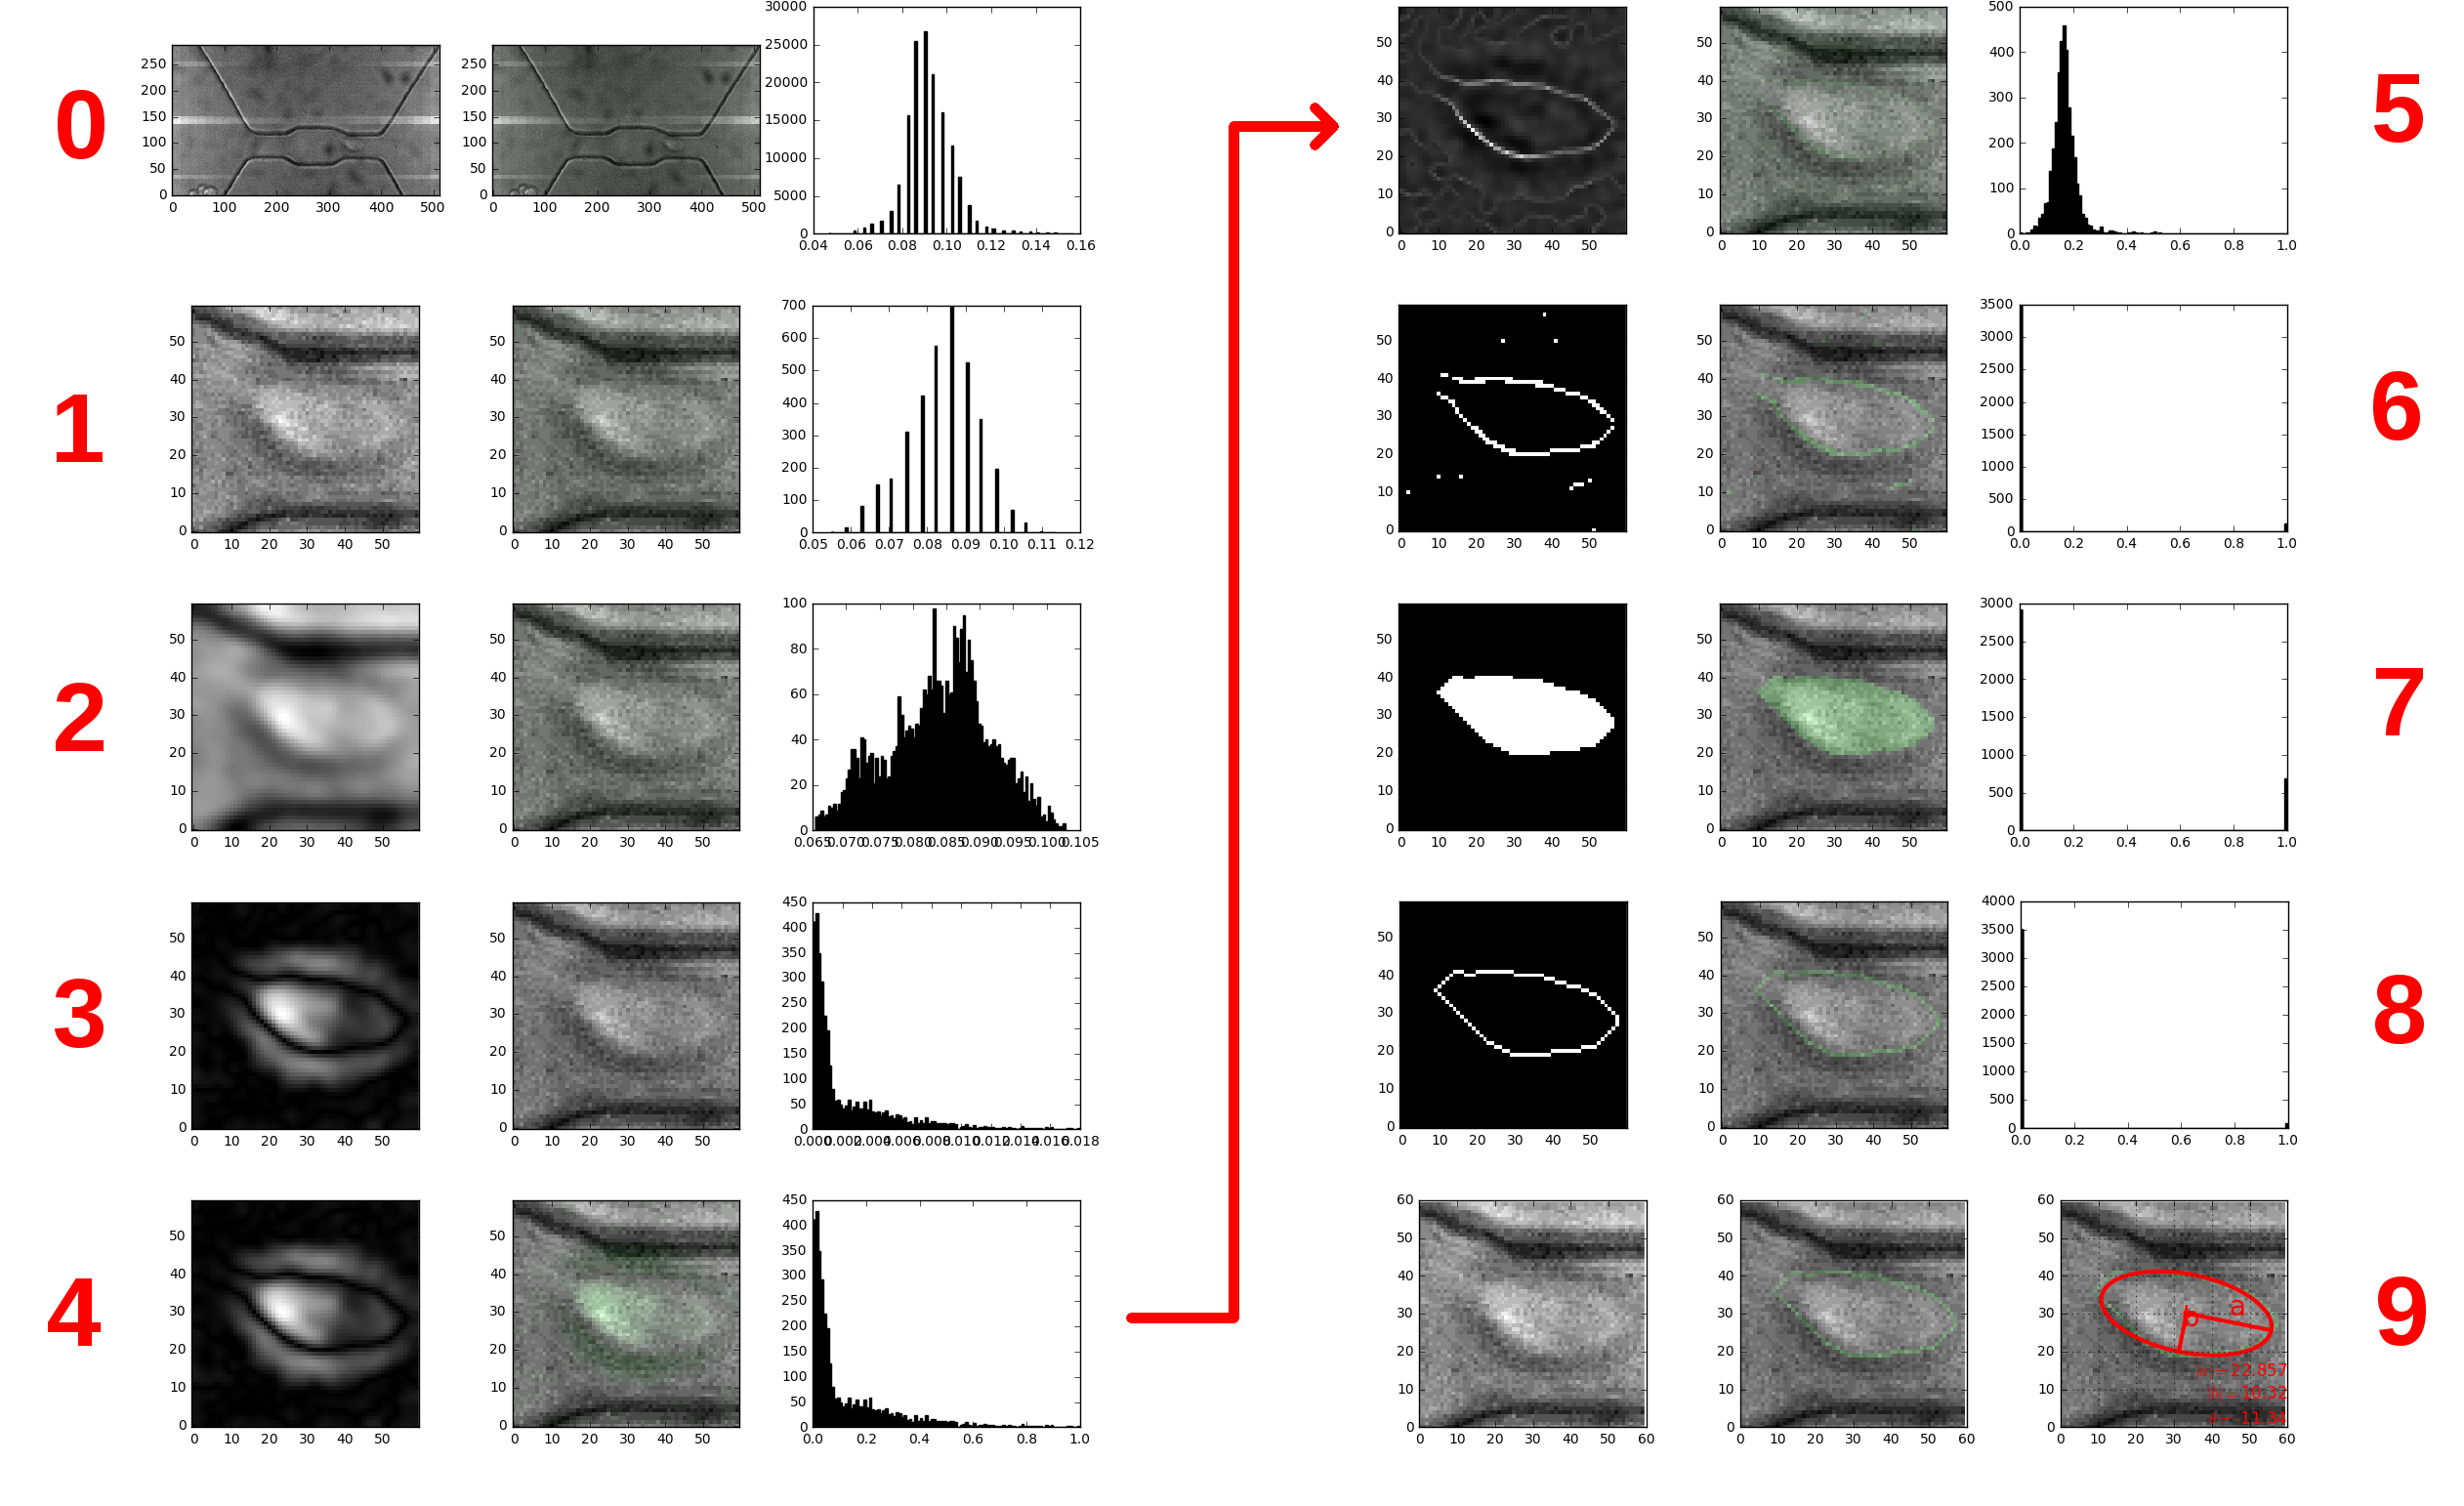
\includegraphics[width=\textwidth]{ellipsefittingprotocol.png}
				\caption{\textbf{Example ellipse fitting protocol for a single detection within a single event.} The left column of each row shows the current image transformation. The central column shows the raw frame with the pixels shaded green with intensity according to the intensity of the pixels in the transformed image. The right column shows pixel intensity in the processed image. \textbf{1: } Raw image. \textbf{2:} Image is cropped in the vicinity of the particle. \textbf{3:} Template image is subtracted off. \textbf{4:} Pixel intensity is rescaled. \textbf{5:} Laplacian derivative. \textbf{6:} Pixel intensity thresholding. Notice the histogram becomes binary distributed. \textbf{7:} Morphological closing of image. \textbf{8:} Image is dilated and subtracted from undilated image, leaving a thin shell around the border of the cell. \textbf{9:} Ellipse is fit to the cell's border.}
				\label{fig:ellipsefittingprotocol}
			\end{figure}

			
			
			While the ellipses could be fit manually by determining the width and height of the channel in each frame, the number of cells observed prohibits this manual measurement. Instead, we devise an image processing pipeline that starts with the raw camera data and results in a calculation of the ellipse fits for every single detection and every single particle passing through the channel. The pipeline works as follows. First, cells are detected in individual frames via a template subtraction method. Then, cells are tracked across frames using a minimum distance approach. These two methods are described in greater detail in chapter \ref{chap:rpim}. After a list of events is determined, ellipses need to be fit to the image of the cell in each frame. A number of preprocessing steps is required to transform the image to a form where this ellipse fitting is possible. One possible ellipse fitting protocol is shown in Fig. \ref{fig:ellipsefittingprotocol}. All processing protocols must reduce the image down to a binary form where the only pixels highlighted are the pixels on the exact boundary of the cell. Operations common to most processing protocols are template subtraction, Gaussian blurring, Laplace derivative transformation, thresholding, and morphological operations such as binary dilation, erosion, and closing. The end result is shown in Fig. \ref{fig:ellipsefittingprotocol}, row 9. Fitting an ellipse to the particle in each frame is useful because many properties of the particle and its translocation can be determined via the ellipse fits. For instance, ellipse fitting yields accurate determination of the central position of the particle, which can be used to accurately determine its trajectory and velocity. Furthermore, once the ellipse is obtained for every frame it is easy to calculate the aspect ratio of the particle during the course of its trajectory and compare with the expectations of the model proposed earlier (Fig. \ref{fig:deformationmotif}.
			
			
	
	\section{Results \& Discussion}
	
		\begin{figure}
			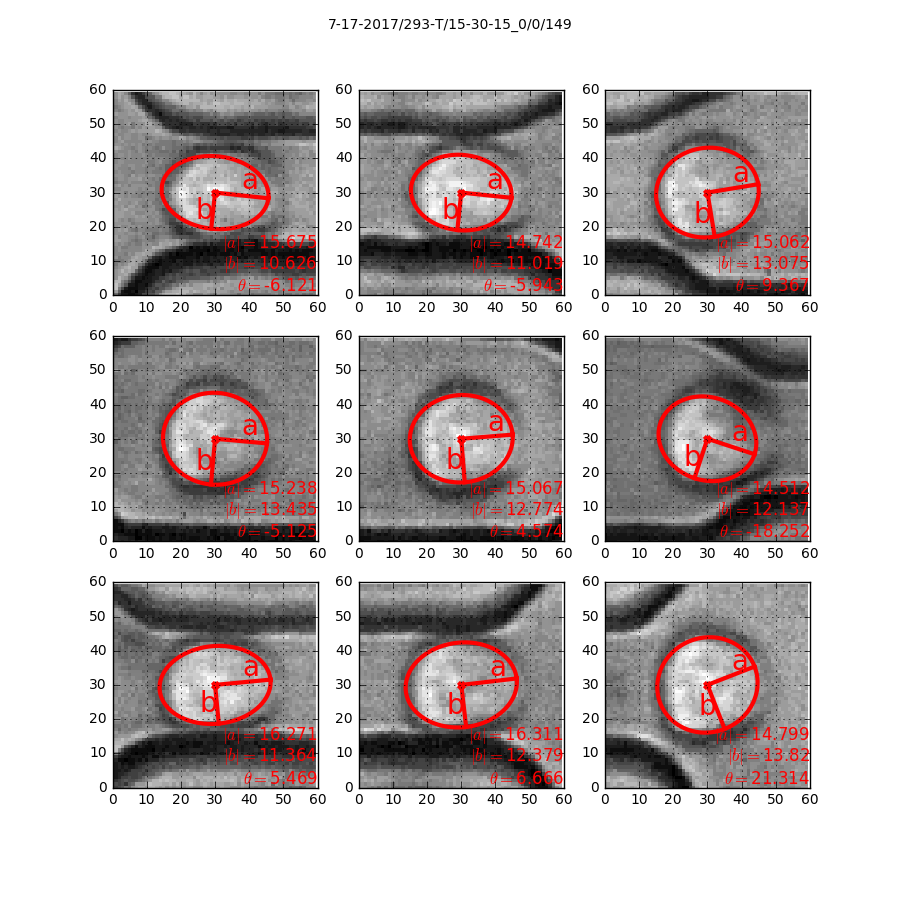
\includegraphics[width=0.5\textwidth]{ellipses.png}
			\caption{\textbf{Ellipse fits for a 293-T cell passing through a $15-30-15 \mu\mathrm{m}$ channel at various positions.} Notice that in the narrow portions of the channel the particle assumes a prolate (axially-elongated) shape, while in the central cavity it assumes an oblate (laterally-elongated) shape, in agreement with the motif presented in Fig. \ref{fig:deformationmotif}}.
			\label{fig:ellipses}
		\end{figure}

	
		The most important question to be answered in the experiments is whether the cells actually deform according to the model proposed. In order to answer this question, we examined specific events to look at their change in aspect ratio as they pass through the channel. Many events consistently show a deformation pattern that subscribes to the model, as shown in Fig. \ref{fig:ellipses}. On the other hand, there were many events that showed modest to little deformation. However, this result is not unreasonable; our model does not suggest that all cells must deform, and indeed there may be cells that are quite resilient to deformations, or cases where the hydrodynamic forces were insufficient to generate significant deformation. However, we never observe a trend opposite to the deformation mode posited, i.e. an oblate-to-prolate transition rather than a prolate-to-oblate transition. This observation suggests that, while the magnitude of the effect may be low in some cases, the effect still occurs.

		

		
		


%%% Local Variables: ***
%%% mode: latex ***
%%% TeX-master: "thesis.tex" ***
%%% End: ***



% These commands fix an odd problem in which the bibliography line
% of the Table of Contents shows the wrong page number.
\clearpage
\phantomsection

% "References should be formatted in style most common in discipline",
% abbrv is only a suggestion.

\bibliographystyle{abbrv}
\bibliography{../../LaTeX/references/references}

% The Thesis Manual says not to include appendix figures and tables in
% the List of Figures and Tables, respectively, so these commands from
% the caption package turn it off from this point onwards. If needed,
% it can be re-enabled later (using list=yes argument).
\captionsetup[figure]{list=no}
\captionsetup[table]{list=no}

% If you have an appendix, it should come after the references.
% The original template (from Trevor) had a custom \appendix command,
% but I found it to break figure/table counters. I'm not sure how
% reliable my fix is, so I ended up reverting back to the standard
% latex version, and renaming the custom command to \myappendix.  You
% can try both and see how things work out:
% 1) Call \appendix once, and then make each appendix a \chapter
% 2) Call \myappendix once, and then make each appendix a \section.

\appendix
\chapter{Appendix Title}


\section{Lorem Ipsum}




%%% Local Variables: ***
%%% mode: latex ***
%%% TeX-master: "thesis.tex" ***
%%% End: ***


\end{document}
